\documentclass[12pt,twoside]{report}
\usepackage{lmodern}
\usepackage{setspace}
\setstretch{1.5}
\usepackage{amssymb,amsmath}
\usepackage{ifxetex,ifluatex}
%\usepackage{fixltx2e} % provides \textsubscript
\ifnum 0\ifxetex 1\fi\ifluatex 1\fi=0 % if pdftex
  \usepackage[T1]{fontenc}
  \usepackage[utf8]{inputenc}
\else % if luatex or xelatex
  \ifxetex
    \usepackage{mathspec}
  \else
    \usepackage{fontspec}
  \fi
  \defaultfontfeatures{Ligatures=TeX,Scale=MatchLowercase}
\fi
% use upquote if available, for straight quotes in verbatim environments
\IfFileExists{upquote.sty}{\usepackage{upquote}}{}
% use microtype if available
\IfFileExists{microtype.sty}{%
\usepackage{microtype}
\UseMicrotypeSet[protrusion]{basicmath} % disable protrusion for tt fonts
}{}
\usepackage[left=3cm, right=3cm, top=2.5cm, bottom=2.5cm]{geometry}
\usepackage{hyperref}
\PassOptionsToPackage{usenames,dvipsnames}{color} % color is loaded by hyperref
\hypersetup{unicode=true,
            pdftitle={LEAP-RE T5.3},
            pdfauthor={Author: Utku B. Demir},
            colorlinks=true,
            linkcolor=Maroon,
            citecolor=Blue,
            urlcolor=blue,
            breaklinks=true}
\urlstyle{same}  % don't use monospace font for urls
\usepackage{longtable,booktabs}
\usepackage{graphicx,grffile}
\usepackage{titlepic}
\makeatletter
\def\maxwidth{\ifdim\Gin@nat@width>\linewidth\linewidth\else\Gin@nat@width\fi}
\def\maxheight{\ifdim\Gin@nat@height>\textheight\textheight\else\Gin@nat@height\fi}
\makeatother
% Scale images if necessary, so that they will not overflow the page
% margins by default, and it is still possible to overwrite the defaults
% using explicit options in \includegraphics[width, height, ...]{}
\setkeys{Gin}{width=\maxwidth,height=\maxheight,keepaspectratio}
\IfFileExists{parskip.sty}{%
\usepackage{parskip}
}{% else
\setlength{\parindent}{0pt}
\setlength{\parskip}{6pt plus 2pt minus 1pt}
}
\setlength{\emergencystretch}{3em}  % prevent overfull lines
\providecommand{\tightlist}{%
  \setlength{\itemsep}{0pt}\setlength{\parskip}{0pt}}
\setcounter{secnumdepth}{5}
% Redefines (sub)paragraphs to behave more like sections
\ifx\paragraph\undefined\else
\let\oldparagraph\paragraph
\renewcommand{\paragraph}[1]{\oldparagraph{#1}\mbox{}}
\fi
\ifx\subparagraph\undefined\else
\let\oldsubparagraph\subparagraph
\renewcommand{\subparagraph}[1]{\oldsubparagraph{#1}\mbox{}}
\fi

%%% Use protect on footnotes to avoid problems with footnotes in titles
\let\rmarkdownfootnote\footnote%
\def\footnote{\protect\rmarkdownfootnote}

%%% Change title format to be more compact
\usepackage{titling}

% Create subtitle command for use in maketitle
\newcommand{\subtitle}[1]{
  \posttitle{
    \begin{center}\large#1\end{center}
    }
}

\setlength{\droptitle}{-2em}

\title{\bftext{LEAP-RE T5.3}}
\usepackage{etoolbox}
\makeatletter
\providecommand{\subtitle}[1]{% add subtitle to \maketitle
  \apptocmd{\@title}{\par {\large #1 \par}}{}{}
}
\makeatother
\subtitle{Scientometric Analysis of Renewable Energy Research-Capacity in Africa \vfill}
\setlength{\droptitle}{-2em}

\vskip
\author{Author: Utku B. Demir}
\date{ZSI-Team: Dietmar Lampert, Elke Dall, Utku B. Demir \vfill 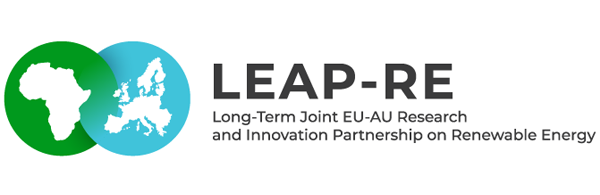
\includegraphics[width=1\linewidth]{./leapre}}


\usepackage{booktabs}
\usepackage{fontspec}
\usepackage{dcolumn}
\usepackage{longtable}

\usepackage{booktabs}
\usepackage{array} 
\usepackage{multirow}
\usepackage{wrapfig}
\usepackage{float}
\usepackage{colortbl}
\usepackage{pdflscape}
\usepackage{tabu}
\usepackage{threeparttable}
\usepackage{threeparttablex}
\usepackage[normalem]{ulem}
\usepackage{makecell}
\usepackage{xcolor}
\usepackage{pdfpages}

\pagestyle{plain}
\raggedbottom 



\let\oldhref\href
\renewcommand{\href}[2]{#2\footnote{\url{#1}}}

\begin{document}
\maketitle

{
\setcounter{tocdepth}{1}
\tableofcontents
}
\hypertarget{abstract}{%
\chapter*{Abstract}\label{abstract}}
\addcontentsline{toc}{chapter}{Abstract}

The present report displays the preliminary results\footnote{The final report of the scientometric analysis will include the inputs of both co-leading organisations of the Task 5.3 MESRS and ZSI. The preliminary report only includes ZSI's work so far.} of the scientometric study on the renewable energy
research-capacity in African countries by focusing on the publications in the 10 years range between 2011-2020. In order to deliver a comprehensive overview, after the analysis of the African countries in their respective African Union regions and international co-publication networks, the study has been broadened into organisational co-publication networks of the selected countries as well as the analysis of the most visible research areas and keywords/ keyword pairs from the selected organisations. Moreover, as a further point of view, renewable energy related publications from the African countries are also categorised under distinct research domains to show the most visible organisational pairings as well as most visible and trending keywords/ keyword pairs in different clusters of scientific areas.


\hypertarget{intro}{%
\chapter{Introduction}\label{intro}}

This study mainly focuses on renewable energy (RE) related research in African countries between 2011-2020. The study has been carried out under the project \href{https://www.leap-re.eu/}{LEAP-RE} (Long-Term Joint European Union - African Union Research and Innovation Partnership on Renewable Energy) \emph{Task 5.3: Strategy for RE research-capacity in Africa} with the co-lead of \href{https://www.mesrs.dz/}{MESRS (Ministry of Higher Education and Scientific Research)} and \href{https://www.zsi.at/}{ZSI (Centre for Social Innovation)}.

The results, which will be displayed in the following chapters, are generated through a cleaned, normalised and recategorised dataset created with the data collected from the \href{https://www.webofscience.com}{Clarivate's Web of Science} databases. A comprehensive discussion about the methods can be found in Chapter \ref{method}.

Following the explanation of the methodology in the next chapter, Chapter \ref{results} displays the results of the study. After showing the overall figures in Section \ref{overall-figures} which include a general overview of the yearly RE-related publication output in the African continent, the most visible countries and organisations as well as the distribution of research domains and areas, Section \ref{regional-analysis} focuses on individual African Union Geographic Regions\footnote{The 5 African Union Geographic Regions; Northern Africa, Western Africa, Central Africa, Eastern Africa, and Southern Africa have been defined by the Organisation of African Unity in 1976 (CM/Res.464QCXVI). A list of countries in each region can
  be found under \url{https://au.int/en/member_states/countryprofiles2}.}. The regional analysis generally deals with the most visible countries in each region as well as their co-publication networks which also include interregional (partnerships with other African countries from other regions) and intercontinental (partnerships with countries from other continents) collaborations. Furthermore, the analysis also focuses on selected countries in each region to display the most visible organisations and organisational co-publication networks as well. The regional analysis also includes at least 1 selected organisation from each selected country to present the most visible research areas and keyword/keyword pair networks on the organisational level. Finally, Section \ref{domain-analysis} approaches the RE research in Africa from another direction and by splitting publications into research domains in order to discuss the most visible co-publication pairings between organisations as well as most visible keywords/ keyword pairs in each distinct cluster of scientific areas.

The report will be delivered in 3 different formats. An HTML-File which includes the whole scope of the report with interactive visualisations, a PDF-File which is content-wise identical to the HTML-File with static visualisations instead of interactive. And a dashboard where the results will be displayed in a compact mode interactively.

\hypertarget{method}{%
\chapter{Methodology}\label{method}}

This chapter mainly deals with the explanation of the methodological definitions, information about the data collection, preprocessing, analysis, and visualisation/ report writing phases.

\hypertarget{definitions}{%
\section{Definitions}\label{definitions}}

\textbf{Research Area/ Research Domain.} Research areas are the scientific fields defined by the Web of Science (WoS). Research domains are the 5 parent categories (Physical Sciences, Technology, Life Sciences \& Biomedicine, Social Sciences, Arts \& Humanities) of the research areas.\footnote{Web of Science's categorization of research areas under research domains can be found under \url{https://images.webofknowledge.com/images/help/WOS/hp_research_areas_easca.html}.}

\textbf{Co-publication}. A publication that has been produced with the collaboration of at least 2 authors from 2 different organisations.

\textbf{Interregional co-publication}. Interregionality in this Report refers to different African countries from different African Union (AU) regions. An interregional co-publication, therefore, is a paper published with the collaboration of at least 2 authors from African organisations from different regions of Africa.

\textbf{Intercontinental co-publication}. Co-publications of at least 2 organisations located on different continents.

\textbf{Relative growth rate}. A simple indicator of how many folds the number of publications has been increased in comparison with the number of publications in the start year (2011). The equation is simply:

\[
rel\_growth\_rate := end\_value/start\_value
\]

\hypertarget{data-source-methodological-steps}{%
\section{Data Source \& Methodological Steps}\label{data-source-methodological-steps}}

The study is based on the data from Clarivate's Web of Science (WoS) databases. After the unification of the collected RE-related keywords by MESRS and ZSI, different types of search queries have been tested on WoS. A search query with over 80\% accuracy for the identification of RE-related research has been determined through sampling processes.

The data collected from WoS databases through the decided search query have been turned into a common dataset for the use of all partners collaborating in the study. The generated dataset has been transformed by preprocessing steps like data cleaning, normalisation, reduction, and categorisation. The normalisation of the organisation names is done with the help of the \href{https://www.grid.ac/}{Global Research Identifier Database (GRID)}.

Following the preprocessing steps, an exploratory data analysis has been carried out and some of the key figures have been visualised to decide for focus points of the study between the partners.

Further data analysis has been carried out accordingly to the joint decision on the report format/ outline planning and visualisations have been designed to work interactively.

\hypertarget{results}{%
\chapter{Results}\label{results}}

Following clarification of the motivation and methodology of the
scientometric analysis on the renewable energy (RE) related research in Africa,
this chapter is dedicated to the presentation of the results under the following
3 sub-chapters:

\begin{enumerate}
\def\labelenumi{\arabic{enumi}.}
\tightlist
\item
  Overall Figures
\item
  Regional Analysis
\item
  Domain Analysis
\end{enumerate}

After delivering a general overview on yearly output, the most visible
countries and organisations as well as distribution of scientific domains and
areas in the RE-related publications in African countries between 2011-2020, \emph{Regional
Analysis} focuses on each of the 5 regions (Northern Africa, Western Africa, Central Africa,
Eastern Africa, Southern Africa)\footnote{A list of the countries in each African Union region can
  be found under \url{https://au.int/en/member_states/countryprofiles2}.} individually. Analysis of the geographic regions
include:

\begin{itemize}
\tightlist
\item
  Most visible countries.
\item
  Regional, interregional, and intercontinental collaboration networks of all countries in the region.
\item
  Collaboration networks of the academic organisations in \emph{selected countries}\footnote{The two deciding factors for the selection were, firstly, the total RE-related
    publication output, and secondly, the relative growth in the number of RE-related publications.}.
\item
  Analysis of the most visible research areas and the correlation network of the
  keyword/keyword pairs in the RE-related publications of the \emph{selected organisations}\footnote{Selection criteria were the same as the criteria for countries.}.
\end{itemize}

\emph{Domain Analysis} approaches RE-related research in Africa from a different perspective
by analysing the publications under the 5 research domains Physical Sciences,
Technology, Life Sciences \& Biomedicine, Social Sciences and Arts \& Humanities\footnote{Web of Science's research area/domain classification can be found under \url{https://images.webofknowledge.com/images/help/WOS/hp_research_areas_easca.html}. Because of the fewer number of publications, Social Sciences and Arts \& Humanities have been analysed together.}. Analysis
of each domain includes:

\begin{itemize}
\tightlist
\item
  Most visible inter-regional/ intercontinental collaborations between academic organisations.
\item
  Most visible and trending keywords/ keyword pairs.
\end{itemize}

\hypertarget{overall-figures}{%
\section{Overall Figures}\label{overall-figures}}

\begin{figure}
 \begin{subfigure}[b]{0.5\textwidth}
% 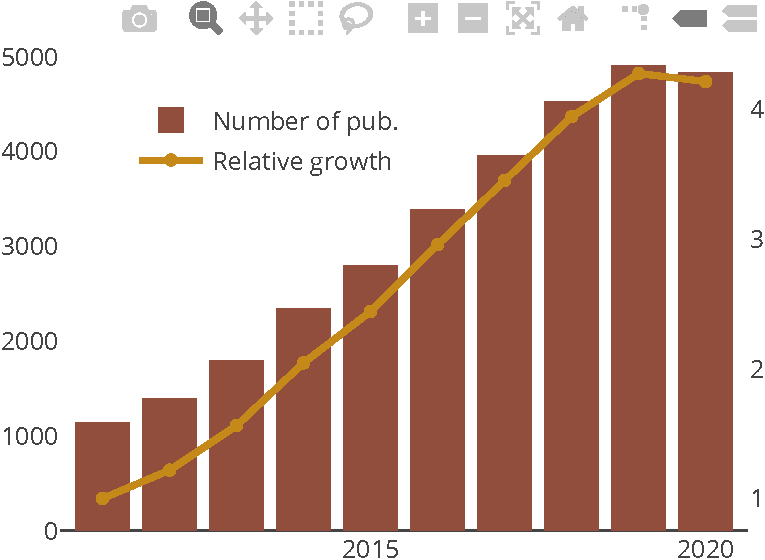
\includegraphics[width=1\linewidth,height=0.5\textheight]{01_bookdown_files/figure-latex/puboty-1} 
\input{pub_oty.pdf_tex}
\end{subfigure}
\caption{Number of RE-related publications in African countries over the years between 2011-2020}\label{fig:puboty}
\end{figure}

African countries have collaborated in approximately 31k renewable energy (RE) related publications in the 10 years range between 2011-2020. The number of those publications has been constantly
increasing until 2019. Slightly declining publication numbers between 2019
and 2020 (see Figure \ref{fig:puboty})
is likely caused by the latency in the database entries\footnote{As the Web of Science support service informs, it might take up to 2 years for a document to be entered into the Web of Science databases.} according to the explanation of Web of Science. Even after including the
possibly incomplete amount of publications in 2020, the number of RE-related publications from
the African countries in total increases from \textasciitilde1.1k in 2011 to \textasciitilde4.8k in
2020 which is an increment by factor \textasciitilde4.2.

\begin{figure}
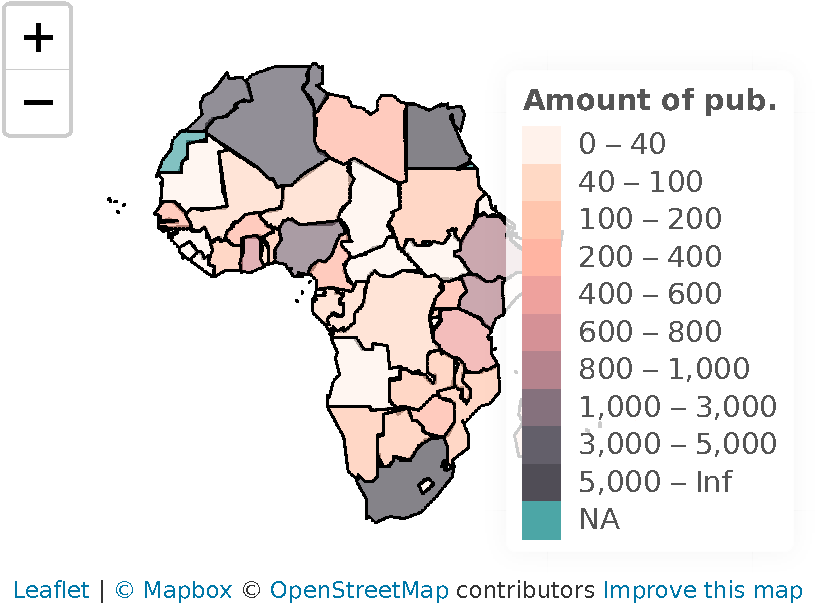
\includegraphics[width=1\linewidth]{01_bookdown_files/figure-latex/choropleth-1} \caption{Total number of RE-related publications in African countries between 2011-2020}\label{fig:choropleth}
\end{figure}

As Figure \ref{fig:choropleth} shows, South Africa and Egypt are the most visible countries with 6.8k and 6.6k RE-related publications respectively. 20 African countries stay under 40 RE-related
publications in total between 2011-2020. The most visible countries are distributed diversely on the continent, however, other than the Northern African countries and South Africa only Nigeria contributed to over 1000 RE-related publications (2252 pub.) between 2011-2020.

Although total publication output is a strong indicator of the most visible countries, it does not show the growth rate in the numbers. African countries that show a high increment rate in the number of publications despite having a relatively lower total amount of publications will be analysed in the following chapter.

\begin{figure}
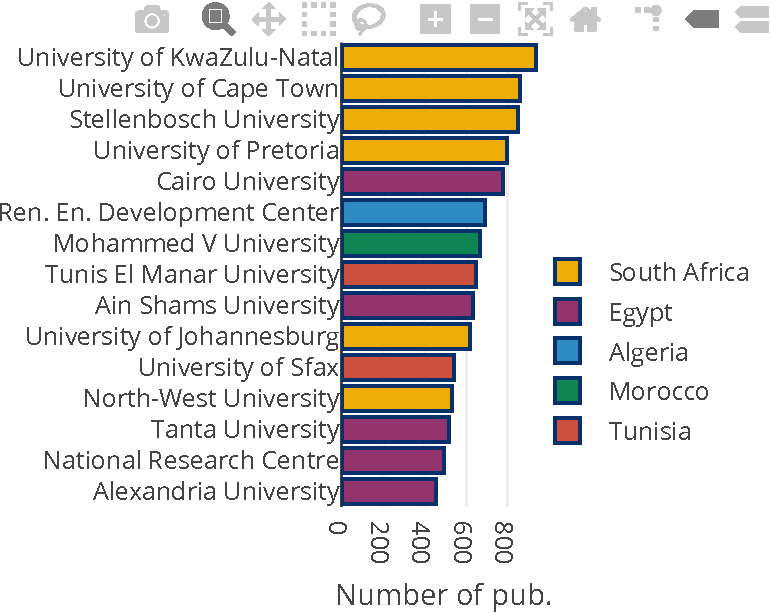
\includegraphics[width=1\linewidth]{01_bookdown_files/figure-latex/orgmv-1} \caption{Most visible 15 African organisations in RE-related publications between 2011-2020}\label{fig:orgmv}
\end{figure}

4 of the most visible 5 organisations (\emph{University of Kwazulu-Natal}, \emph{University of Cape Town}, \emph{Stellenbosch University}, and \emph{University of Pretoria}) in RE-related publications are located in South Africa. Each of them has close to or over 800 publications between 2011-2020, Cairo University from Egypt is following them with \textasciitilde780 publications. 4 other Egyptian institutions; namely Ain Shams University, Tanta University, National Research Centre of Egypt and Alexandria University are also among the 15 most visible organisations.

\emph{Tunis El Manar University} and the \emph{University of Sfax} from Tunisia are also in the most visible 15 organisations with \textasciitilde650 and \textasciitilde550 RE-related publications and \emph{Mohamed V University}, the only organisation from Morocco in the list has \textasciitilde670 RE-related publications.

Although most of the visible organisations are in general universities, the only organisation from Algeria in the most visible 15 organisations, namely \emph{Renewable Energy Development Center} is an institution completely dedicated to RE-related research. The total number of RE-related publications of \emph{Renewable Energy Development Center} is \textasciitilde700 between 2011-2020.

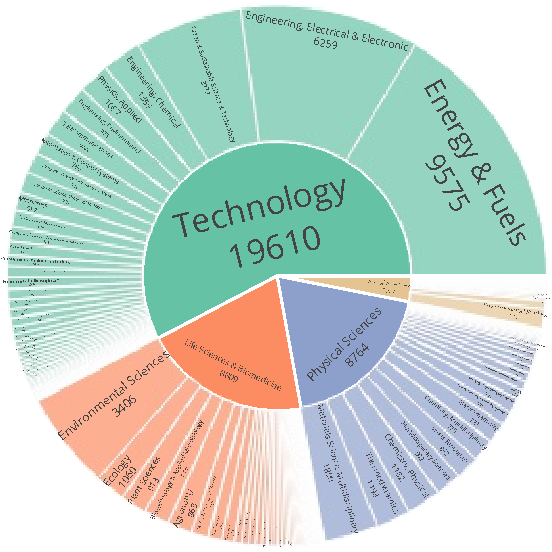
\includegraphics{01_bookdown_files/figure-latex/resdomains-1.pdf}\footnote{A single publication may be associated with multiple research domains/ areas. The sum of the number of publications in individual research domains/areas does not add up to the total number of publications.}

Over 50\% of the RE-related publications are associated with research areas from the \emph{Technology} domain. \emph{Energy \& Fuels} is the most visible research area in total followed by \emph{Electrical \& Electronic Engineering}. Other Engineering fields like \emph{Chemical, Environmental, Mechanical Engineering} are also among the visible research areas. Multidisciplinary discipline \emph{Green \& Sustainable Science \& Technology} is the 3. most visible research area in total.

Life Science \& Biomedicine and Physical Sciences have a similar number of publications (\textasciitilde8800 pub. both). \emph{Environmental Science} and \emph{Ecology} from Life Sciences \& Biomedicine as well as \emph{Multidisciplinary Materials Science} and \emph{Thermodynamics} from Physical Sciences are also in the 10 most visible research areas.

Social Sciences (1325 pub.) is also not absent in the RE-related publications of African organisations. \emph{Environmental Studies} is the most visible research area in this domain with 663 publications.

The 5. research domain Arts \& Humanities include only 45 publications, therefore, this domain will be analysed together with Social Sciences in Chapter \ref{domain-analysis} Domain Analysis.

\hypertarget{regional-analysis}{%
\section{Regional Analysis}\label{regional-analysis}}

Following the overall figures of the RE-related publications in Africa, this section introduces the geographical regions of Africa to broaden the analysis further. Focusing on different regions of Africa prevents the over-representation of already relatively more visible countries in terms of publications and also enables a detailed analysis for individual countries and organisations.

\begin{figure}
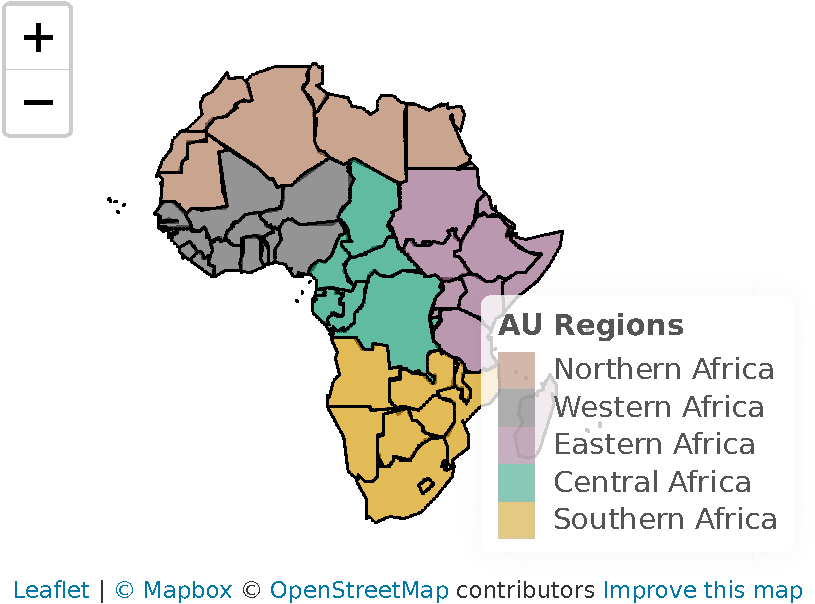
\includegraphics[width=1\linewidth]{01_bookdown_files/figure-latex/auregions-1} \caption{African Union geographic regions}\label{fig:auregions}
\end{figure}

To determine the African regions, this study uses \href{https://au.int/en/member_states/countryprofiles2}{the categorisation provided by African Union}. A presentation of the African Union regions can be seen in Figure \ref{fig:auregions}.

As Figure \ref{fig:afrcouplt} summarizes, 4 of the most visible African countries in the RE-related publications are from Northern Africa. South Africa has the highest number of RE-related publications (\textasciitilde6900) between 2011-2020, only other member country of Southern Africa in the most visible 15 countries is Zimbabwe with 230 RE-related publications between 2011-2020. Nigeria, Ghana, Senegal from Western Africa; Ethiopia, Kenya, Tanzania, Uganda from Eastern Africa; and Cameroon, the only country from Central Africa, are among the 15 most visible countries following the most visible 5 countries.

\begin{figure}
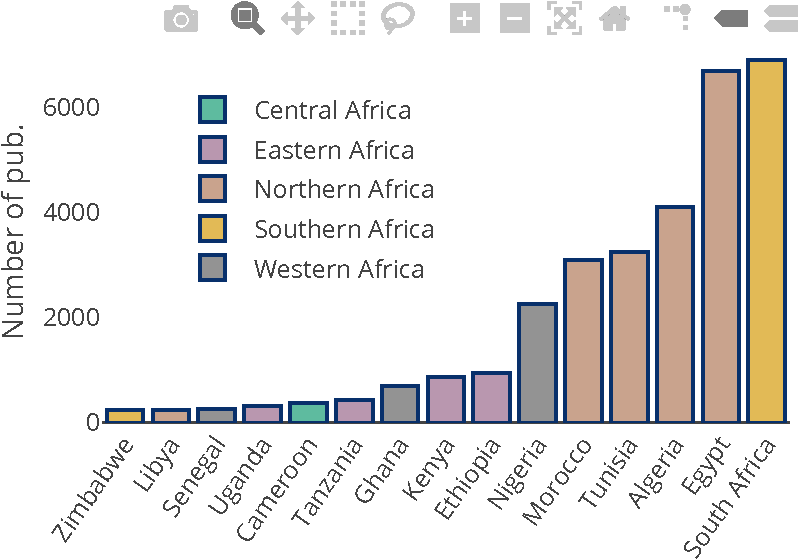
\includegraphics[width=1\linewidth]{01_bookdown_files/figure-latex/afrcouplt-1} \caption{The most visible 15 African countries in  RE-related publications between 2011-2020}\label{fig:afrcouplt}
\end{figure}

\hypertarget{northern-africa}{%
\subsection{Northern Africa}\label{northern-africa}}

\begin{figure}
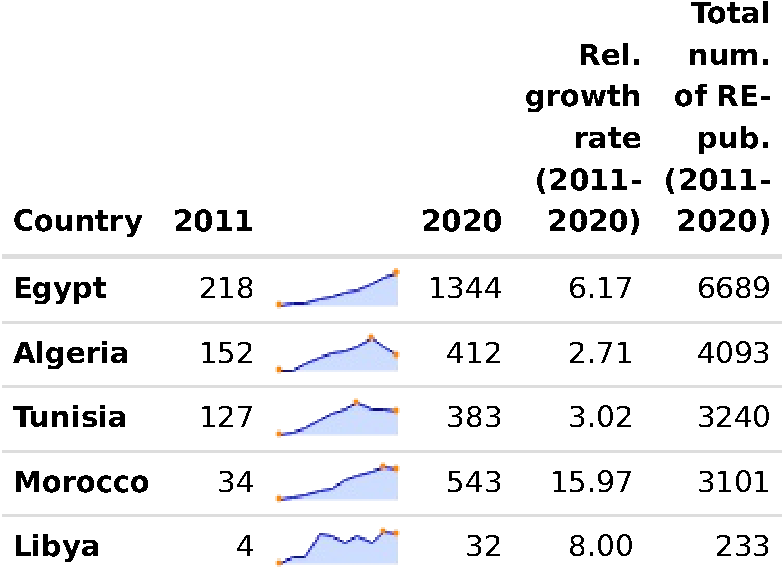
\includegraphics[width=1\linewidth]{01_bookdown_files/figure-latex/tables-natable-1} \caption{RE-related publication output in the most visible Northern African countries}\label{fig:tables-natable}
\end{figure}

Member countries of Northern Africa have collaborated approximately in half of
the total number of all RE-related publications (17116 publications out of 31099) in Africa between 2011-2020. 4 of the 5 most visible African countries in RE-related publications are from the
northern region; namely Egypt, Algeria, Tunisia and Morocco.

As Table \ref{fig:tables-natable}
presents, all of the Northern Africa countries increased their number of RE-related
publications until 2017. Although, as discussed in the previous chapter, slight declines in the number of publications between 2019-2020 are most likely caused by the delay of document entry into the Web of Science databases, Algeria and Tunisia show an earlier start of
the decline in their number of publications starting in 2017 and 2018 respectively. In the
case of Libya, however, volatility in the number of publications
is expected as their total publication outputs are relatively lower.

Another important observation is in the relative growth rates,\footnote{Relative growth rate value in this report does not indicate a percentage as
  it is usually calculated, instead the equation is simply \(end\_value/start\_value = growth\_rate\).} Morocco's number of
RE-related publications in 2020 are approximately 16 times higher than the number in 2011.
This growth rate is not only the highest in Northern Africa but in the whole continent among the most visible countries in RE-related research.

\begin{figure}

\includegraphics[width=1\linewidth]{01_bookdown_files/figure-latex/nanet-1} \caption{Co-publication network of Northern African countries in RE-related publications between 2011-2020}\label{fig:nanet}
\end{figure}

RE-related co-publications of the Northern African countries show a rich international network but the collaboration with other African regions seems to be relatively less dense. Only African countries from other regions which have co-published over 25 RE-related papers with Northern African countries are South Africa (28 pub.) and Nigeria (26 pub.).

Egypt, the most visible country in Northern Africa in terms of RE-related publications, plays a central role in the network with \textasciitilde6.6k publications in total. The relatively uniform distributed co-publication network of Egypt includes over 10 EU-27 countries as well as a number of countries from other regions of the world like the USA, China, India, United Kingdom. Egypt's strongest link in the co-publications, however, is with organisations from Saudi Arabia.

Tunisia, Algeria and Morocco have relatively high numbers of collaborations with French organisations with 751, 881 and 601 co-publications respectively. France in general is the most visible EU-27 country in the RE-related co-publications with African countries. Out of France's \textasciitilde3250 RE-related co-publications with African countries \textasciitilde2350 of those have been published with the collaboration of Northern African countries whereas Algeria and Tunisia being the most visible Northern African countries in those collaborations. The closest following EU-27 country in terms of RE-related co-publications is Spain (\textasciitilde580 out of \textasciitilde820 co-publications with African countries) and Germany (\textasciitilde490 out of 1334 co-publications with African countries).

The 4 mentioned Northern African countries so far, Egypt, Algeria, Tunisia and Morocco are co-publication-wise relatively well interconnected, however, Libya stays out of the co-publication cluster in Northern Africa, from Libya's 233 RE-related publications in the last 10 years none of the Northern African countries had over 25 co-publications with Libya. Instead, Libya's most visible collaborators are United Kingdom (38 co-pub.) and Malaysia (29 co-pub.).

Following the given analysis of RE-related publication outputs in Northern Africa;
Egypt, Algeria and Morocco have been chosen for the deeper analysis of the individual countries.
While Egypt and Algeria hold the highest numbers of RE-related publications in the northern
region, Morocco has been mainly chosen for the high growth rate in the number of publications.

\hypertarget{egypt}{%
\subsubsection{Egypt}\label{egypt}}

\textbackslash begin\{figure\}
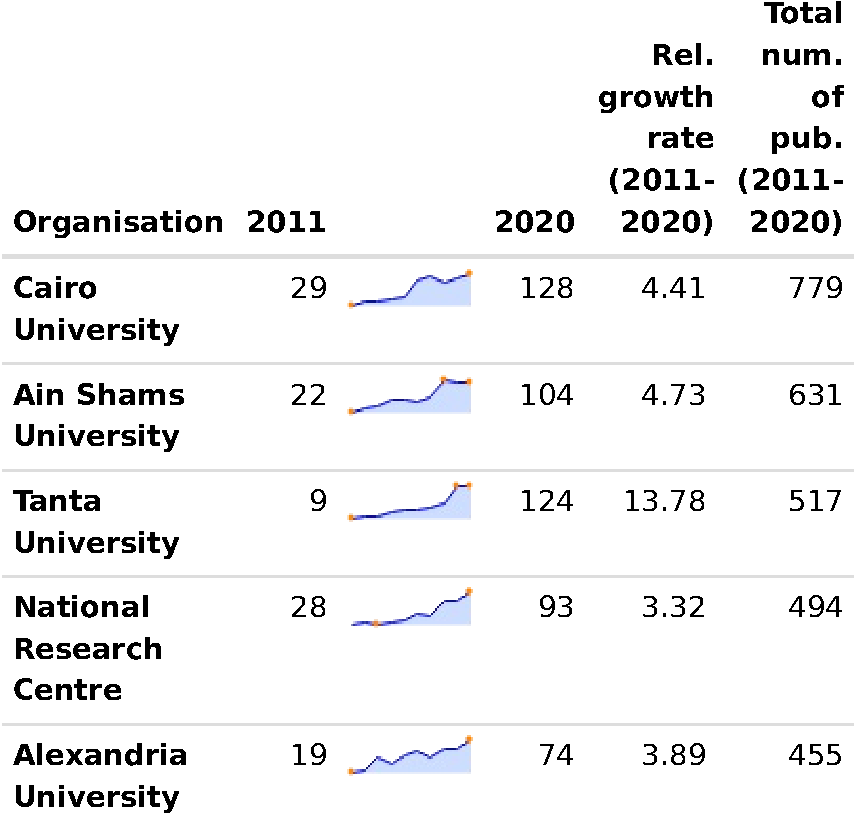
\includegraphics[width=0\linewidth]{01_bookdown_files/figure-latex/egyptorgtable-1}

The most visible Egyptian organisation in the RE-related publications is \emph{Cairo University} with a total of 779 publications between 2011-2020. All of the most visible 5 organisations of Egypt display a fairly linear growth in the number of RE-related publications. However, Ain Shams University and Tanta University show a stagnation between 2019-2020 which might be caused by the delay of document entries into the Web of Science system as mentioned above. Furthermore, Tanta University, which had yearly fewer than 50 RE-related publications until 2016, published in 2019 and 2020 \textasciitilde125 RE-related papers, this is a growth rate of \textasciitilde14 fold with respect to the 9 publications in 2011.

\begin{figure}
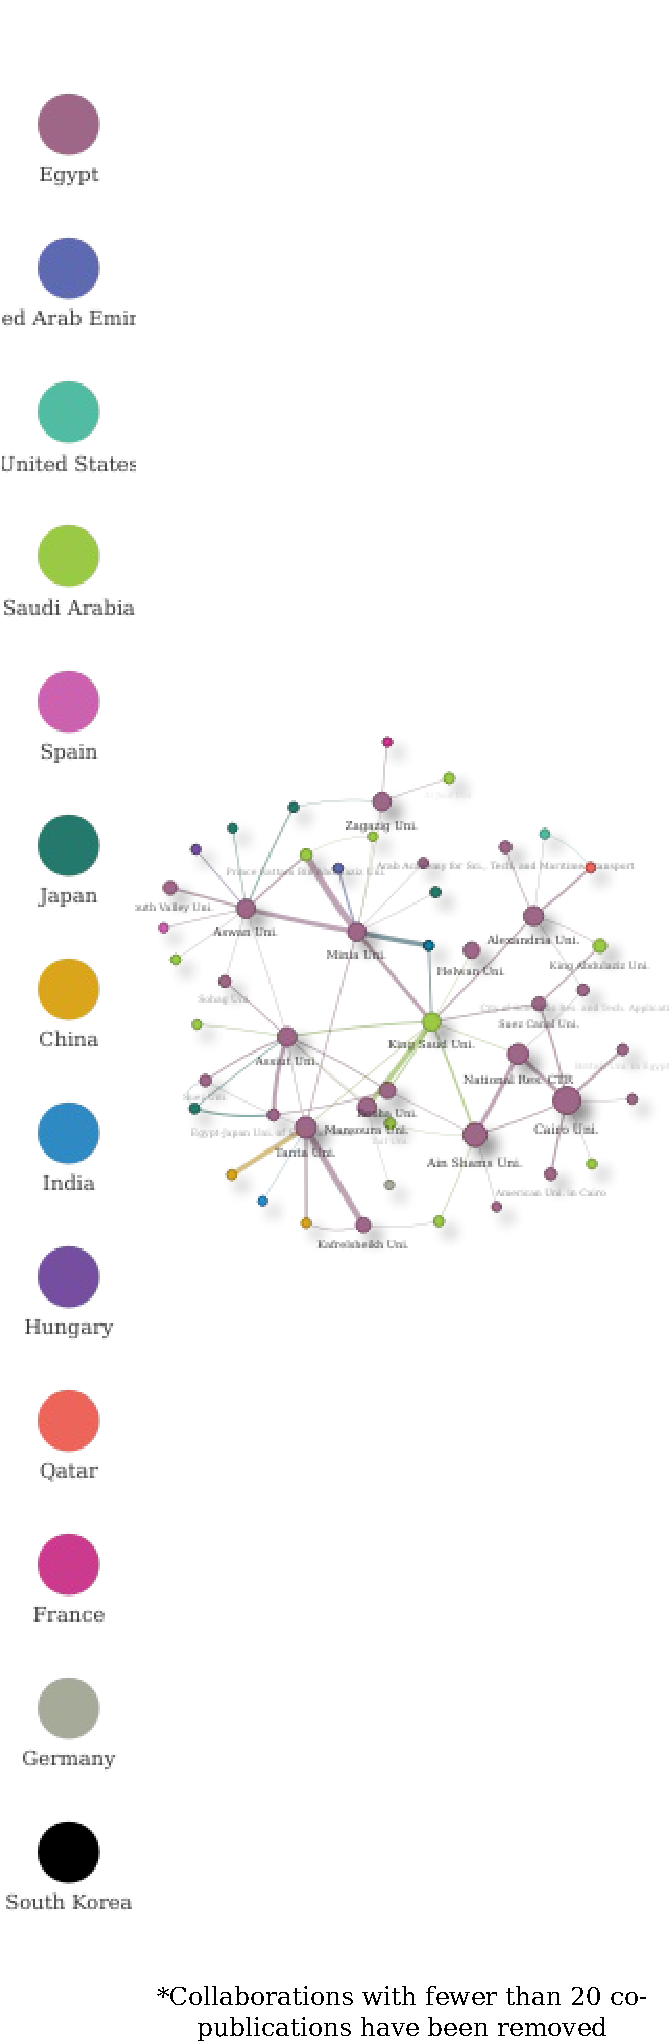
\includegraphics[width=1\linewidth]{01_bookdown_files/figure-latex/egyptnet-1} \caption{Co-publication network in RE-related publications in organisations from Egypt between 2011-2020}\label{fig:egyptnet}
\end{figure}

The co-publication network of Egyptian organisations shows a relatively dense collaboration structure between \emph{Cairo University}, \emph{Ain Shams University} and \emph{National Research Centre} of Egpyt. \emph{National Research Centre} has over 50 co-publications with each of the other universities in that cluster. \emph{Cairo University} is also in the centre of 4 other Egyptian organisations; namely \emph{Suez Canal Uni.}, \emph{British Uni. in Egypt}, \emph{Zewail City of Sci. Tech} and \emph{American Uni. in Cairo}, with over 20 co-publications each.

Other visible collaboration links are between \emph{Minia} and \emph{Aswan Universities} with over 50 publications and between \emph{Tanta} and \emph{Kafrelsheikh Universities} with over 70 publications together. In general, collaborations with organisations from Saudi Arabia are highly visible in the network, especially \emph{King Saud University} is a central node in the network with \textasciitilde400 RE-related co-publications with Egyptian organisations.

Other than that, East Asian organisations also have a visible presence in the co-publication network of Egypt. \emph{Tanta University}'s collaborations with Chinese institutions \emph{Jiangsu Uni.} and \emph{Huazhong Uni} include 60 and 40 co-publications respectively. Several Japanese universities have collaborations with \emph{Aswan University}, \emph{Zagazig University}, \emph{Assiut University}, \emph{Suez University}, \emph{Egypt Japan University} and \emph{Minia University} with over 20 co-publications each. \emph{Minia University}'s collaboration with South Korean institution \emph{JeonBuk National University} also includes 60 RE-related co-publications between 2011-2020.

Visible organisations from EU-27 countries are \emph{Université Bourgogne Franche-Comté} of France (over 25 co-publications with \emph{Zagazig University}), \emph{Ruhr University Bochum} from Germany (22 co-publications with \emph{Mansoura Uni.}), \emph{Budapest University of Technology and Economics} from Hungary and the \emph{University of Jaen} from Spain (both over 25 co-pub. with \emph{Aswan University}).

\hypertarget{cairo-university}{%
\paragraph{Cairo University}\label{cairo-university}}

\begin{figure}
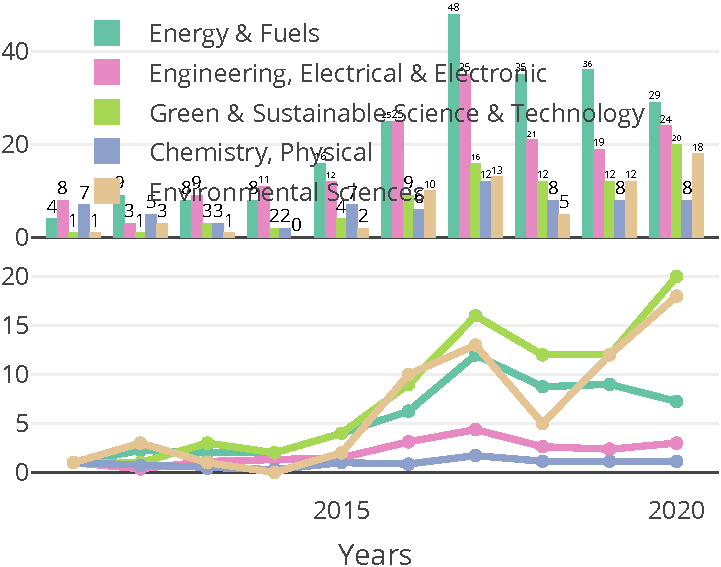
\includegraphics[width=1\linewidth]{01_bookdown_files/figure-latex/cairobarline-1} \caption{Absolute and relative growth of the most visible research areas in RE-related publications of Cairo University between 2011-2020}\label{fig:cairobarline}
\end{figure}

Looking into the most visible research areas of \emph{Cairo University}, out of 779 publications in total, the most visible research areas are aligning with the most visible research areas in RE-related publications from African countries in general. \emph{Energy \& Fuels}, as well as \emph{Electrical \& Electronic Engineering} are the most visible research areas in Cairo University, however, the number of RE-related in those areas are not growing in the last years. After the spike in 2017 with \textasciitilde50 publications, the number of publications from \emph{Energy \& Fuels} has fallen to \textasciitilde30 publications in 2019 and 2020. \emph{Green \& Sustainable Science \& Technology} and \emph{Environmental Sciences} on the other hand display relatively steady growth in numbers. Considering there was only 1 from each area in 2011, \textasciitilde20 RE-related publications in 2020 makes those the fastest growing research areas in the RE-related publications of Cairo University.

\begin{figure}
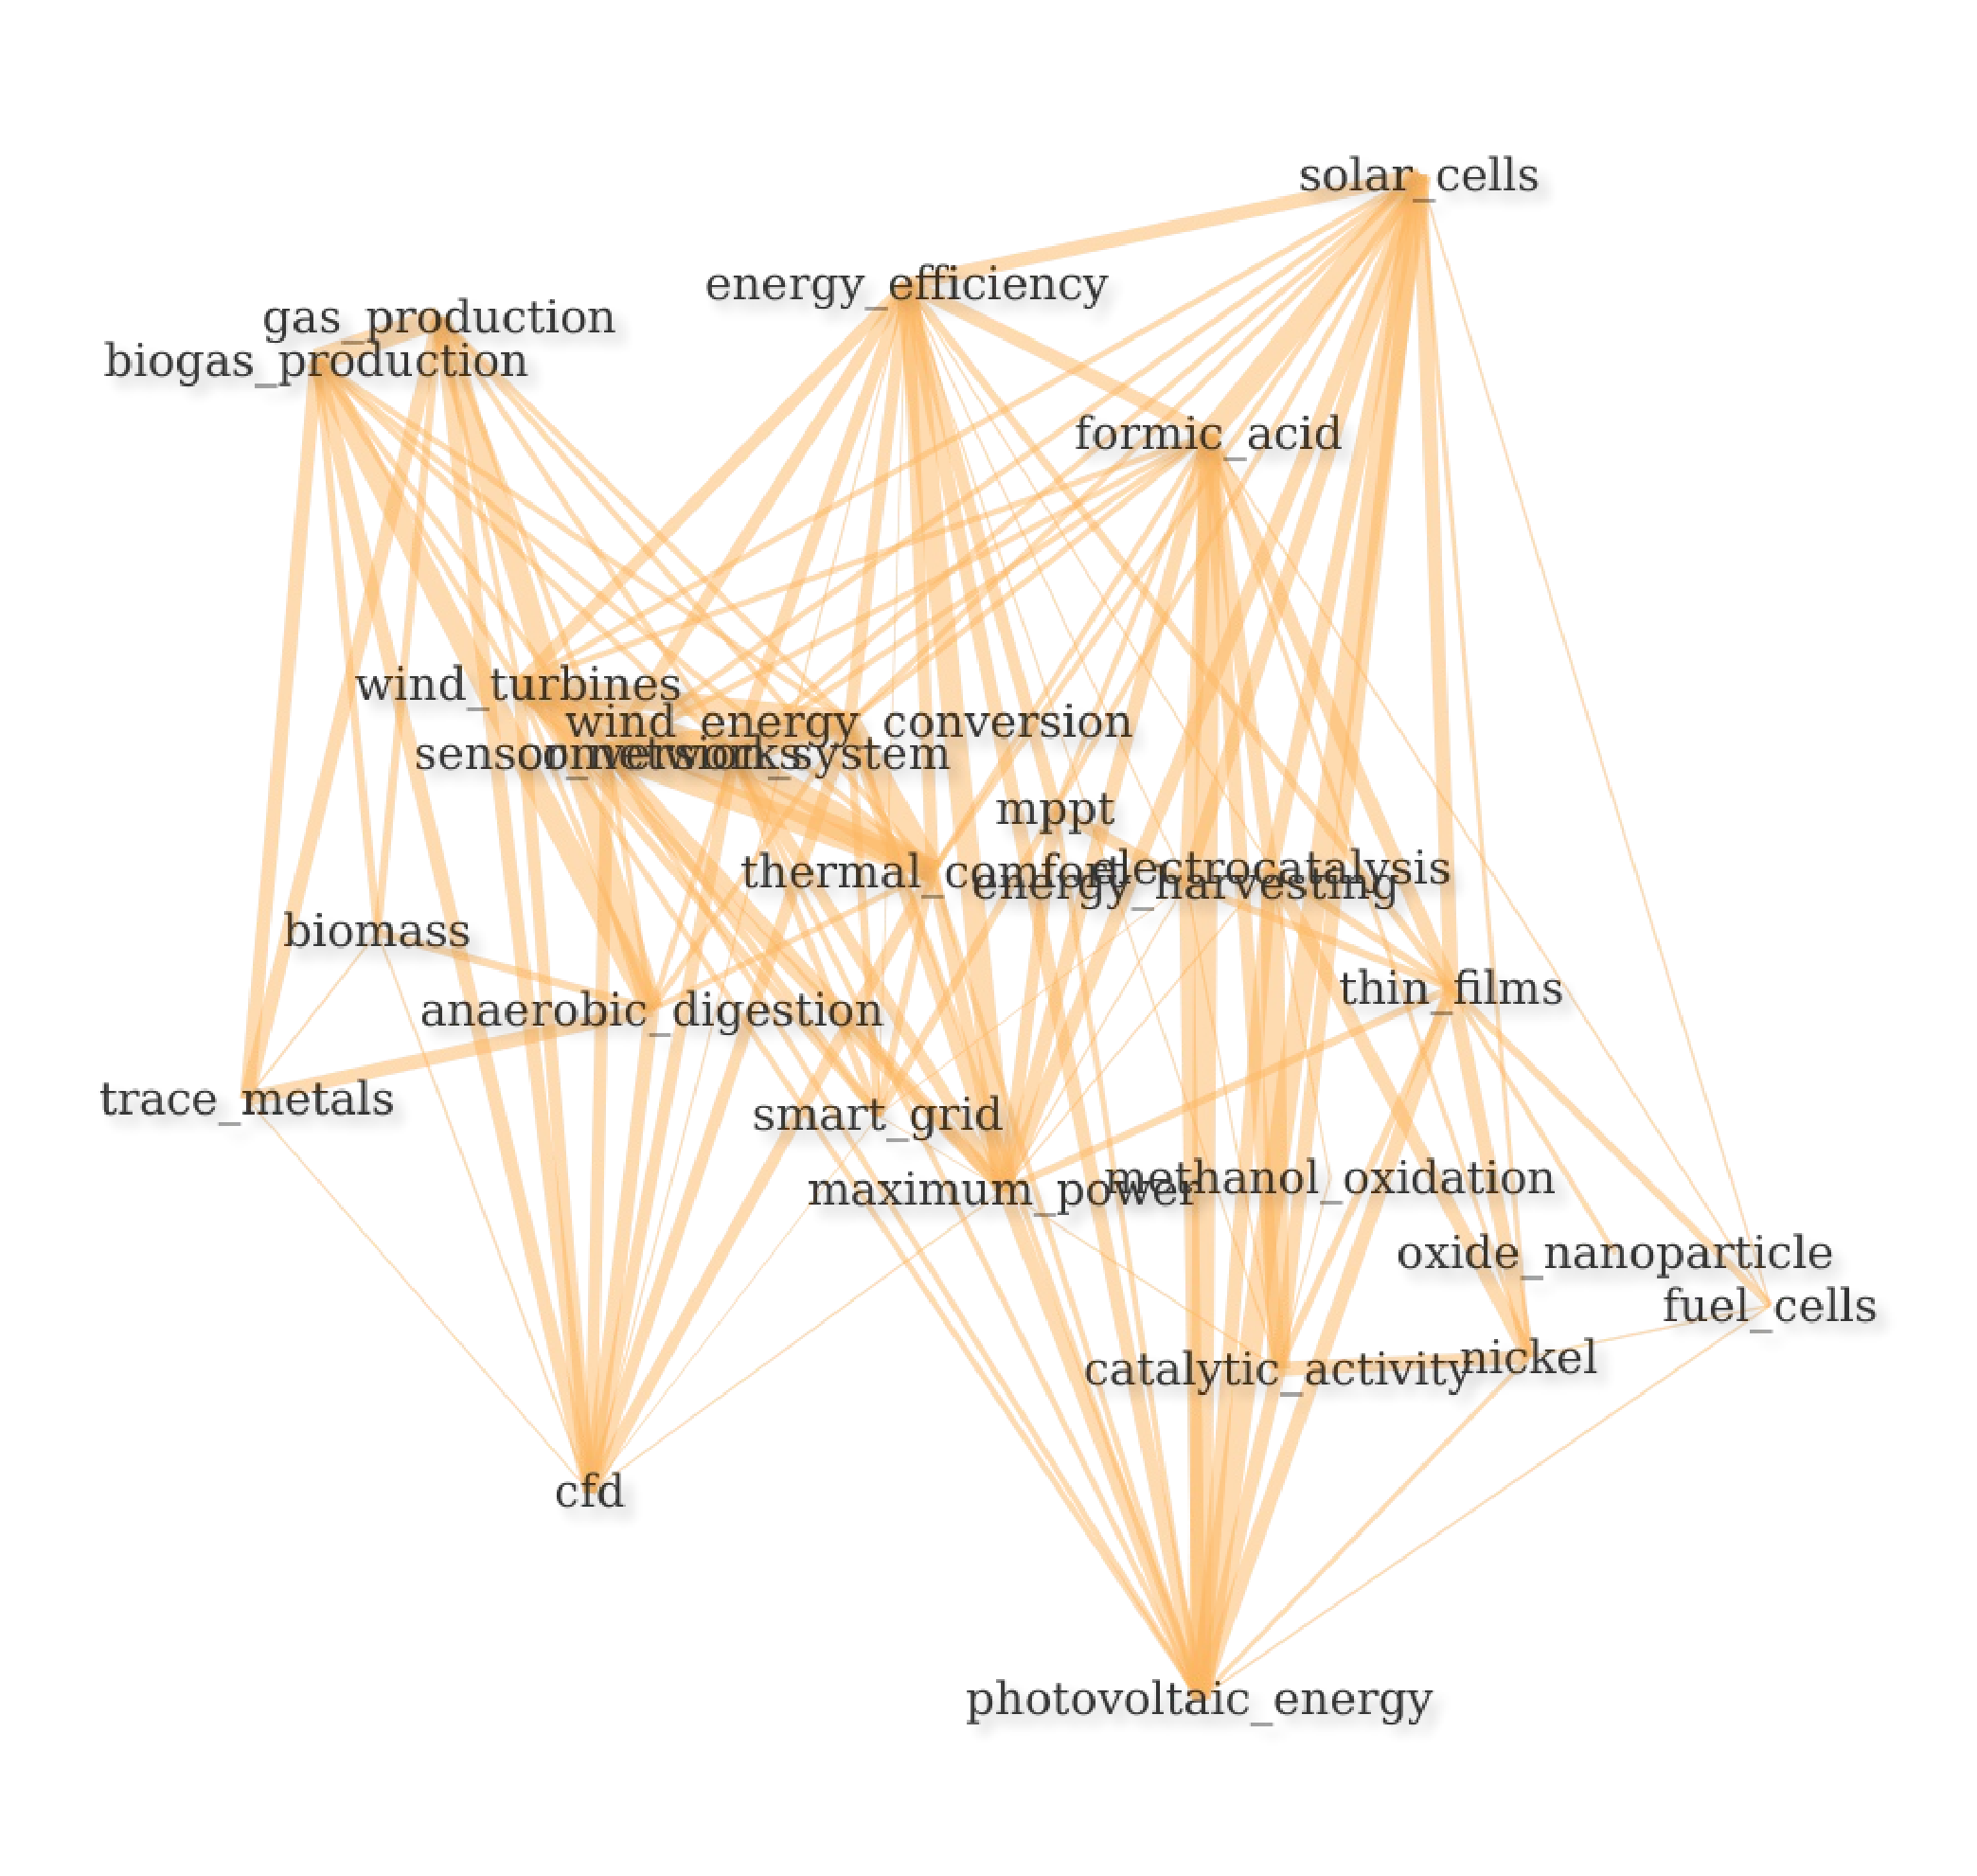
\includegraphics[width=1\linewidth]{01_bookdown_files/figure-latex/cairongramnetwork-1} \caption{Keyword/keyword pair correlation network in RE-related publications of Cairo University}\label{fig:cairongramnetwork}
\end{figure}

Figure \ref{fig:cairongramnetwork} displays the correlation network between the most common keywords and keyword pairs in the RE-related publications of \emph{Cairo University}. As the clusters on the network graph indicate, there is a strong emphasis on solar energy, photovoltaic systems related keywords in \emph{Cairo University}'s publications which is widely the case in African countries. In relation, substances and technologies aiming to improve the efficiency of the effectiveness of solar cells like formic acid, MPPT (Maximum Power Point Tracking, an algorithmic DC-DC converter that increases the efficiency of photovoltaic cells) are also among the visible keyword pairs. Other clusters include wind energy-related keywords as well as biogas/biomass related keywords. The approaches like electrocatalysis that aims to increase the output of solar and wind energy are also often mentioned in the RE-related publications of \emph{Cairo University}.

\hypertarget{algeria}{%
\subsubsection{Algeria}\label{algeria}}

\textbackslash begin\{figure\}
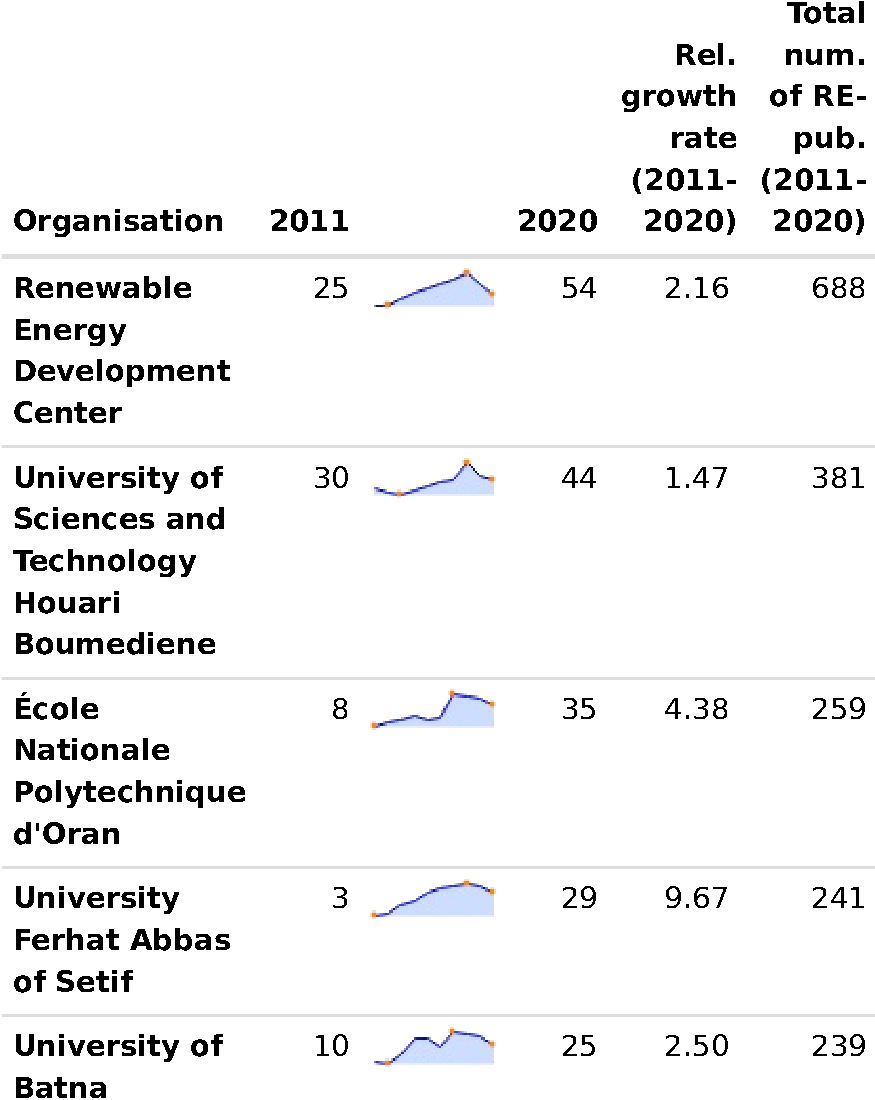
\includegraphics[width=1\linewidth]{01_bookdown_files/figure-latex/algeriaorgtable-1}

\emph{Renewable Energy Development Center}, Algeria's dedicated institution for RE-related research is the most visible organisation in the country with \textasciitilde690 publications. However, the number of RE-related publications of the institution is falling after a spike in 2018 with 127 publications. Although the latency in the record entry process in WoS databases might be causing a proportion of the decline, the number of publications in 2020 seems to be less than half of the number in 2018 (54 pub.).

\emph{Houari Boumediene University of Sciences} is another Algerian institution that publishes RE-related papers consistently. A similar decline in the number of publications like in the case of \emph{Renewable Energy Development Center} can be observed in the publications of \emph{Houari Boumediene University of Sciences} after 2018 (from 75 publications to 44 publications in 2020). \emph{École Nationale Polytechnique d'Oran University}, \emph{Ferhat Abbas of Setif} and the \emph{University of Batna} are other organisations with similar numbers of RE-related publications (259, 241, 239 pub. respectively), each of those has increased their yearly RE-related publication output to \textasciitilde30. The decline in the number of publications after \textasciitilde2018 can be observed in all of the most visible 5 organisations of Algeria.

\begin{figure}
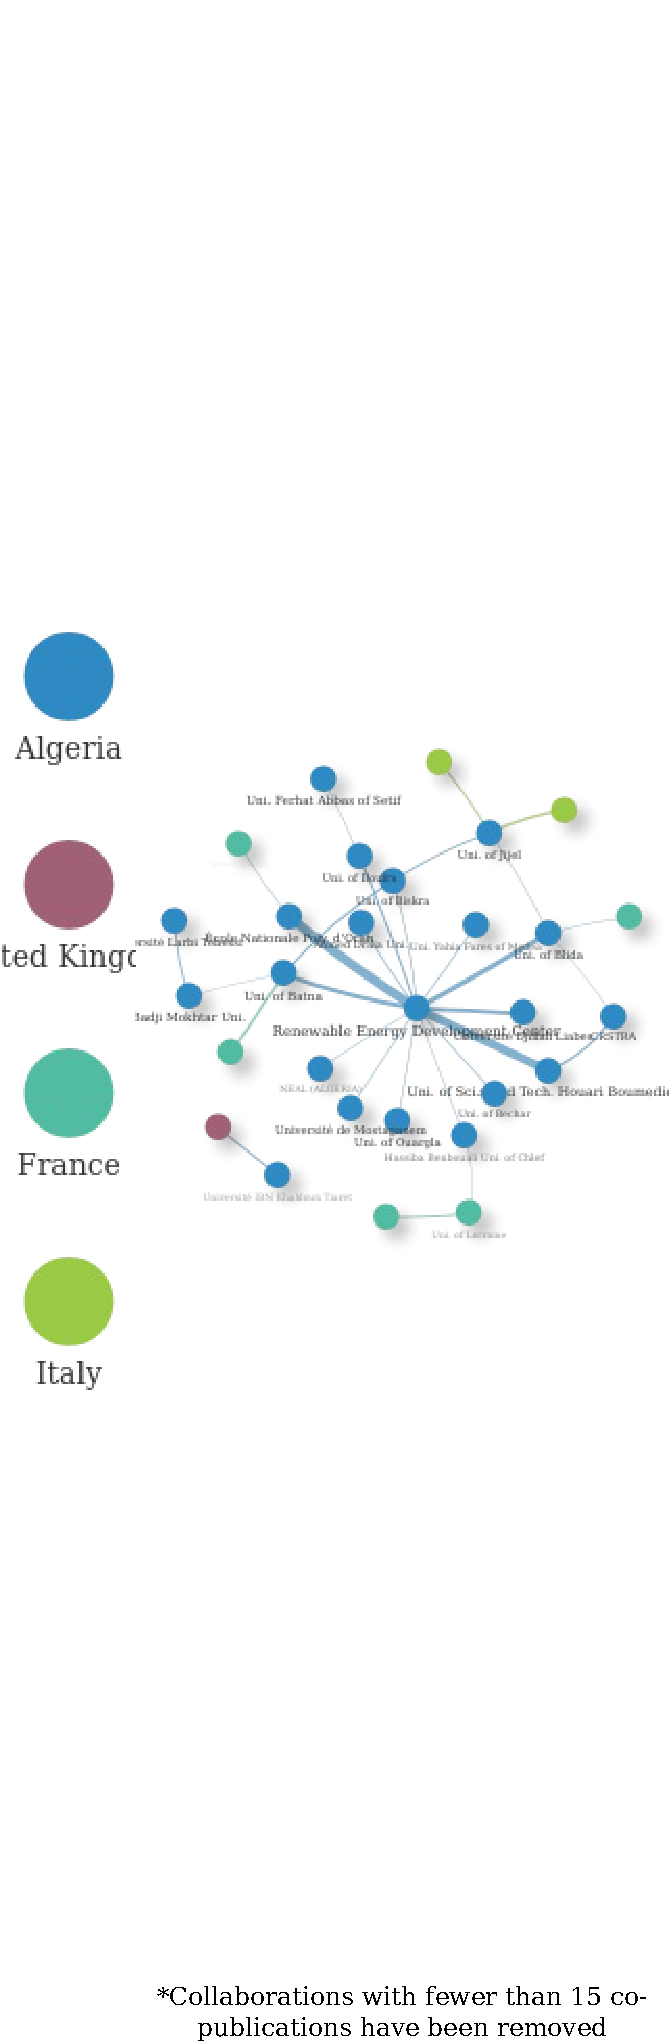
\includegraphics[width=1\linewidth]{01_bookdown_files/figure-latex/algerianet-1} \caption{Co-publication network in RE-related publications in organisations from Algeria between 2011-2020}\label{fig:algerianet}
\end{figure}

Co-publication network of Algerian organisations mostly gathered around \emph{Renewable Energy Development Center}, the to RE-related research dedicated institution collaborates with a number of other Algerian academic institutions, from which 14 of the collaboration links include close to or over 20 co-publications. The most visible collaborations with \emph{Renewable Energy Development Center} are with \emph{Houari Boumediene University of Sciences} and \emph{École Nationale Polytechnique d'Oran University}, both with an output of over 60 co-publications.

Most of the international collaborators with more than 25 co-publications with Algerian institutions are French, the collaboration between \emph{University of Batna} and \emph{University of Picardy Jules Verne} is the most visible one with 27 co-publications between 2011-2020. \emph{University of Jijel} collaborates often with Italian institutions like \emph{University of Trieste} (23 co-pub.) and \emph{International Centre for Theoretical Physics} (28 co-pub.). Other than that, \emph{University of Hertfordshire} is the only organisation from the UK that has more than 20 RE-related co-publications with an Algerian organisation (\emph{University Ibn Khaldon}) between 2011-2020.

\hypertarget{renewable-energy-development-center}{%
\paragraph{Renewable Energy Development Center}\label{renewable-energy-development-center}}

\begin{figure}
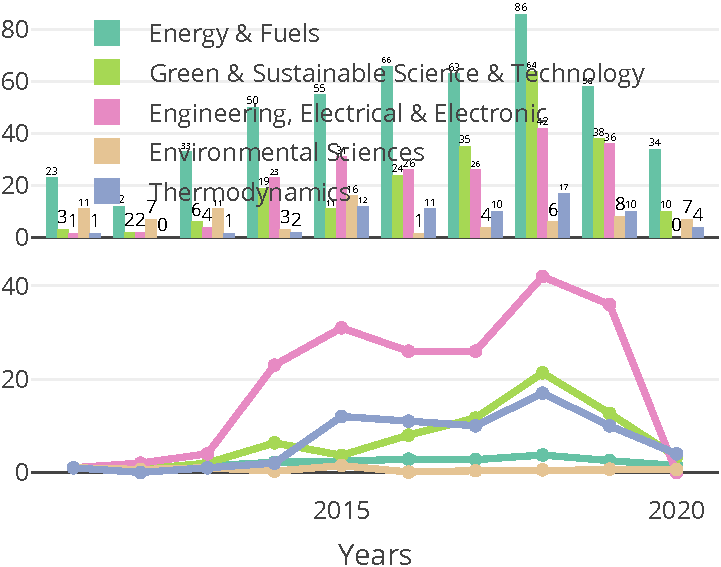
\includegraphics[width=1\linewidth]{01_bookdown_files/figure-latex/redecbarline-1} \caption{Absolute and relative growth of the most visible research areas in RE-related publications of Renewable Energy Development Center between 2011-2020}\label{fig:redecbarline}
\end{figure}

The most visible research areas in the RE-related publications of \emph{Renewable Energy Development Center} are \emph{Energy \& Fuels} and \emph{Green \& Sustainable Science in Technology}. All of the most visible 5 research areas are declining in numbers after 2018 which indicates that there was at least some effect caused by the delayed entry of the publications into the Web of Science databases. However, even after the possibly missing publication from the last years Thermodynamics seems to be becoming one of the consistently visible research areas in the RE-related publications of Renewable Energy Development Center. Environmental Sciences which already included relatively high number of publications in 2011 (11 pub.) is also becoming a consistent area despite having volatile yearly number of publications between 2014-2017.

\begin{figure}
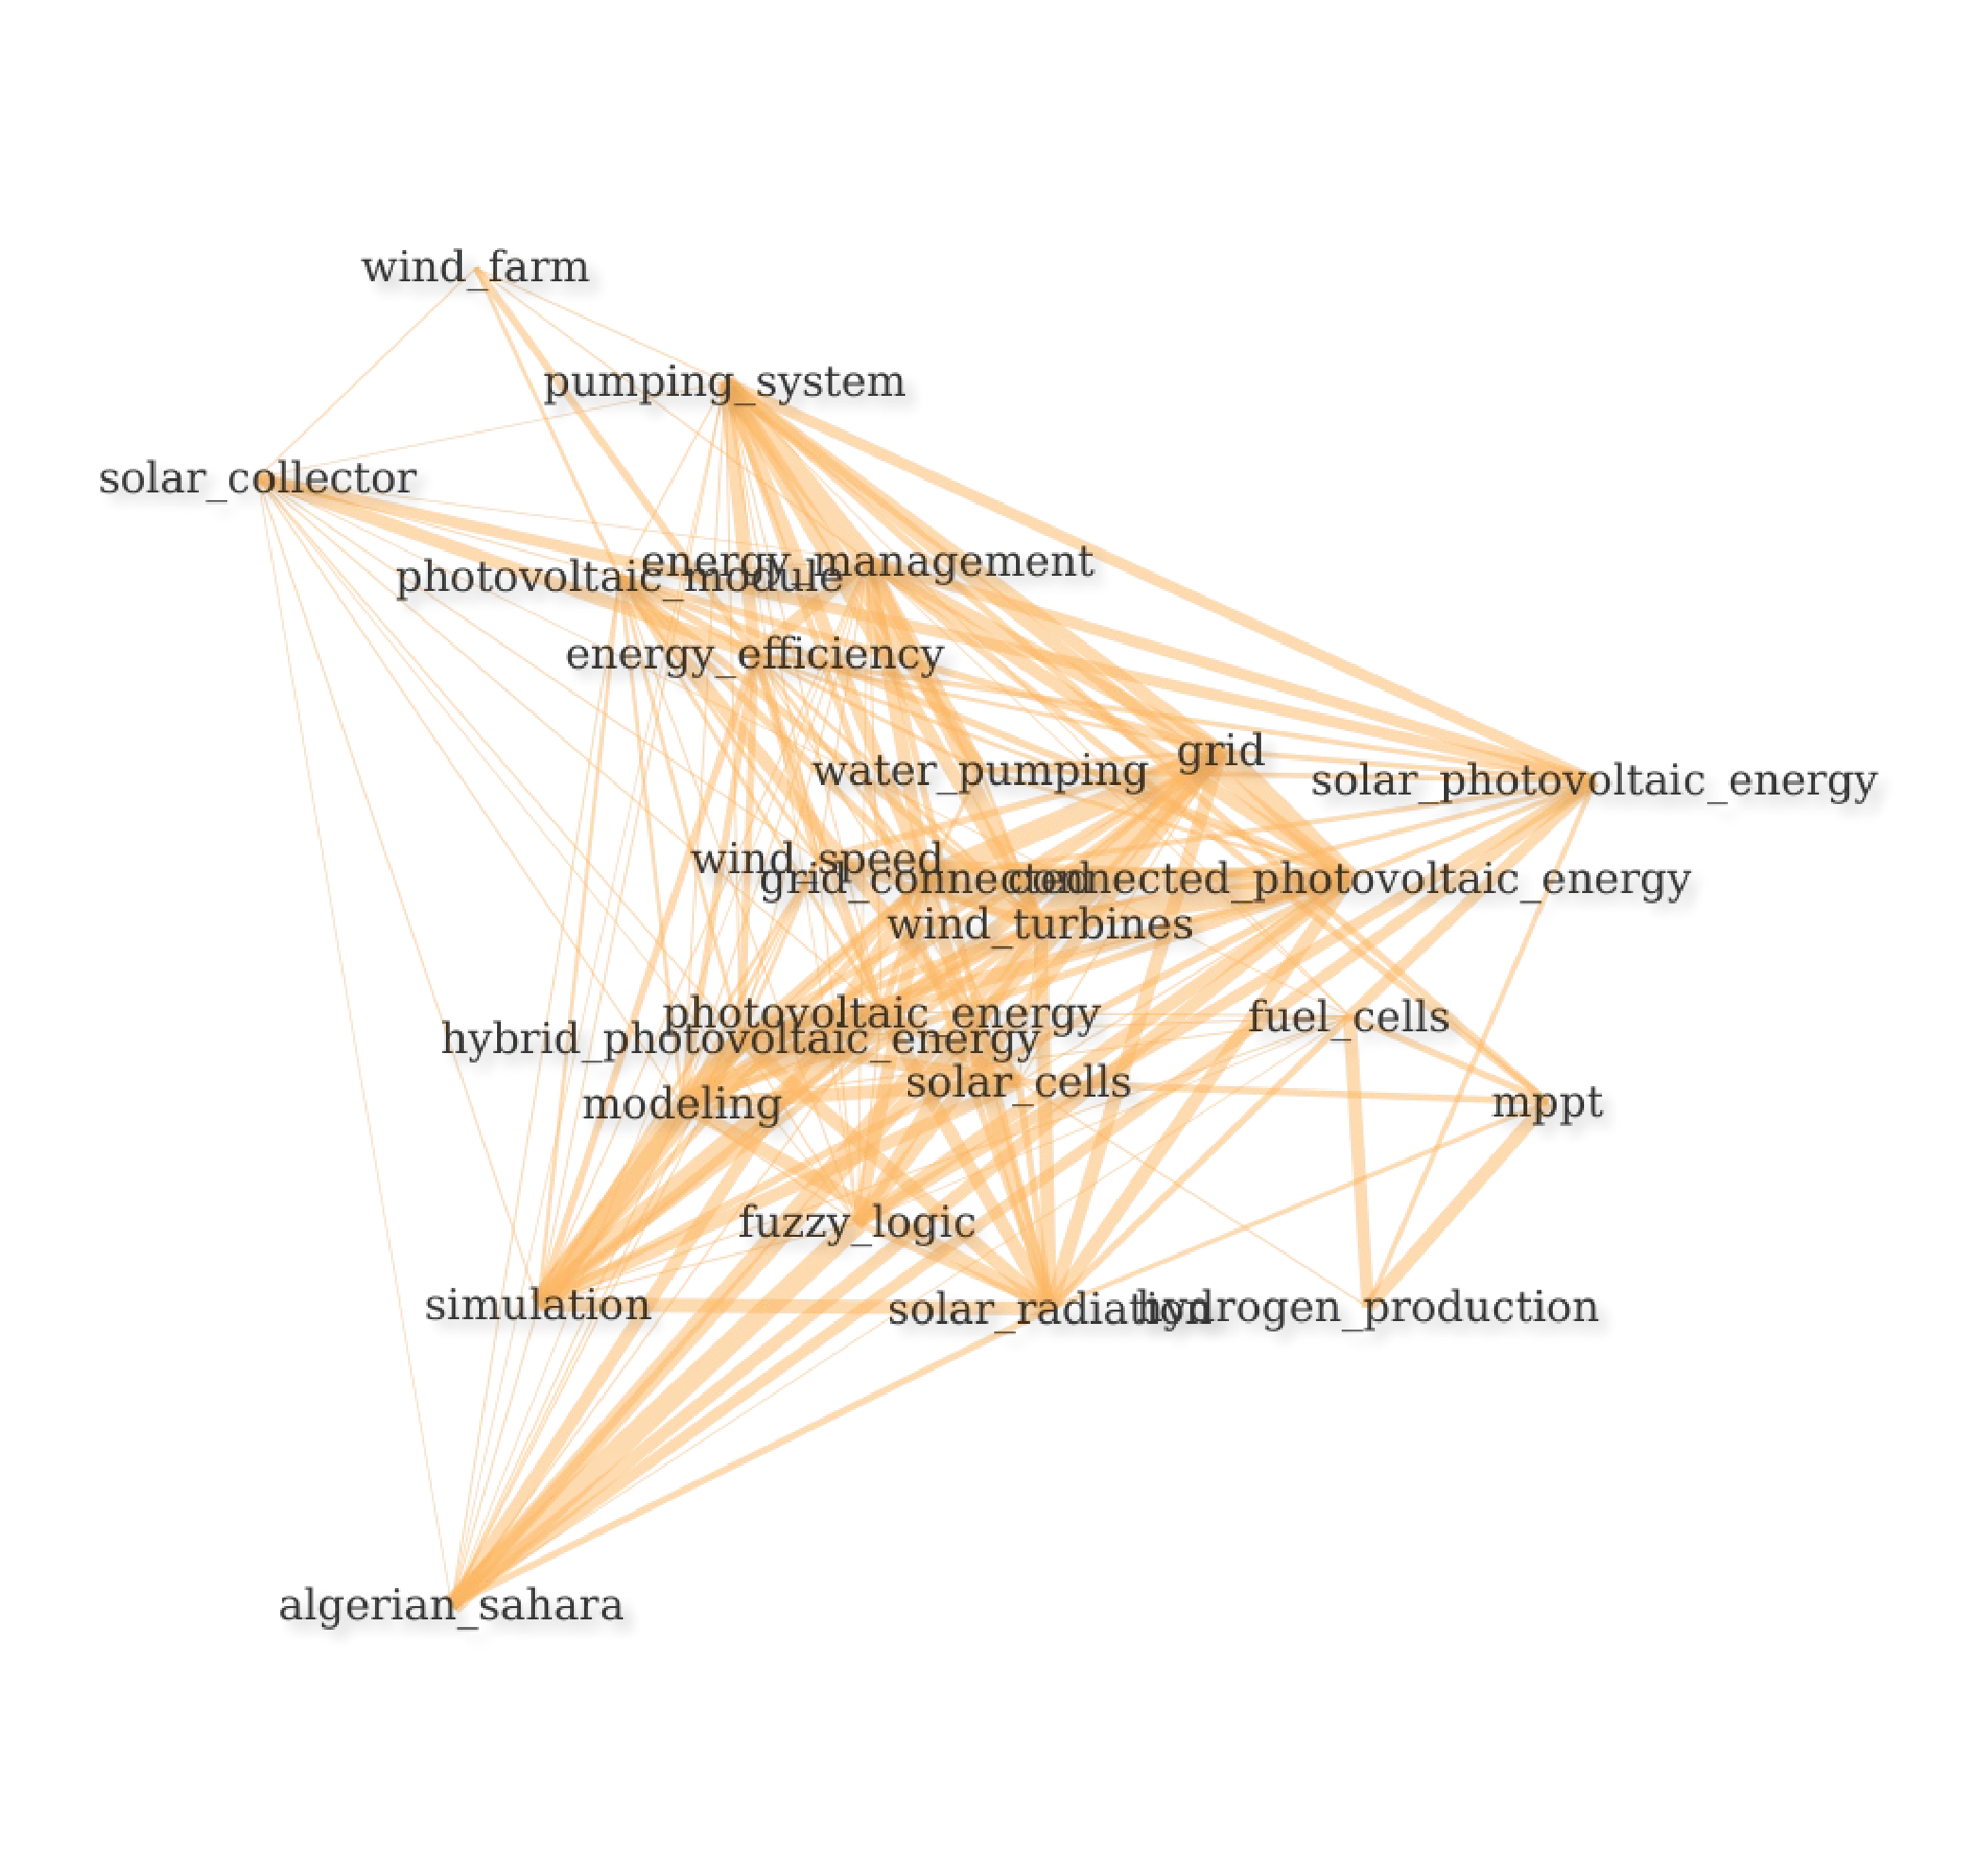
\includegraphics[width=1\linewidth]{01_bookdown_files/figure-latex/redecgramnetwork-1} \caption{Keyword/keyword pair correlation network in RE-related publications of Renewable Energy Development center}\label{fig:redecgramnetwork}
\end{figure}

Keyword/keyword pair correlation network also displays heavily solar energy-related topics. We are seeing that the exploitation of Algerian Sahara for solar energy production is an often reoccurring theme in the publications of \emph{Renewable Energy and Development Center}. Wind energy-related topics are also emphasized in the most visible keyword pairs.

The reason, why water pumping systems are relatively highly correlated with the solar energy keywords is the recent technological advances to build photovoltaic water pumps. Algeria is one of the most active countries in Africa that search for photovoltaic water pumping solutions especially for the isolated sites which are not connected to an electrical grid (see \protect\hyperlink{ref-benghanem2007}{Benghanem and Arab} (\protect\hyperlink{ref-benghanem2007}{2007})\footnote{The citations are chosen to inform the reader about possibly unfamiliar concepts. Therefore, instead of citing the publications from the very institution (which are often too technical for the purpose of this study), we have decided to seek more informative papers directed to an uninitiated audience.} for further reading).

\hypertarget{morocco}{%
\subsubsection{Morocco}\label{morocco}}

\textbackslash begin\{figure\}
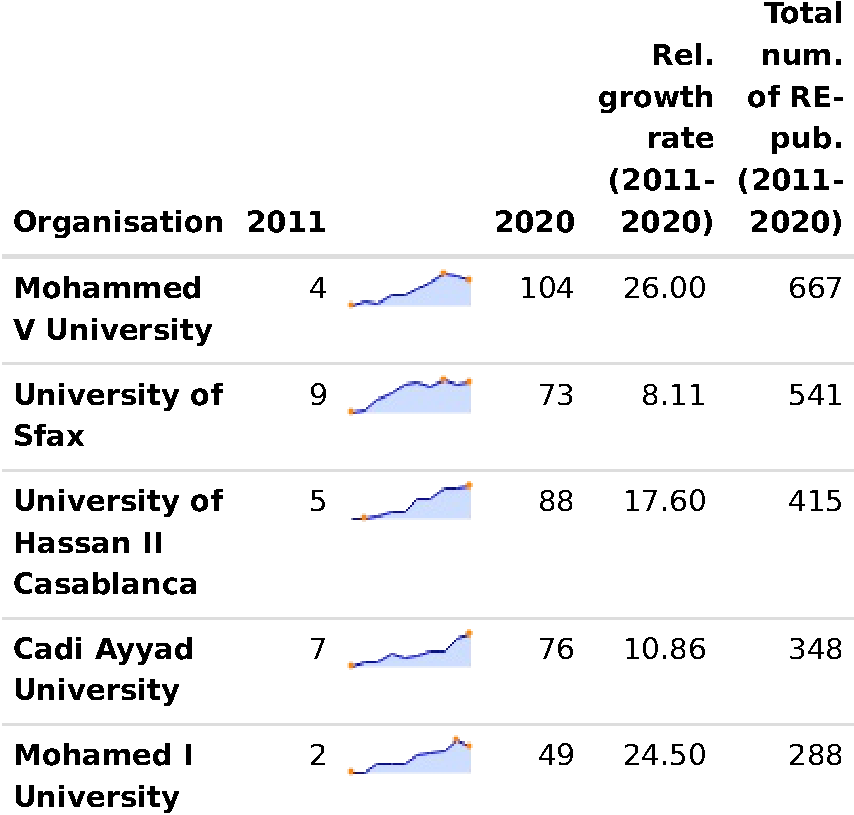
\includegraphics[width=0\linewidth]{01_bookdown_files/figure-latex/moroccoorgtable-1}
Morocco has the most rapidly growing number of publications in the 15 most visible African countries in RE-related publications with having 543 publications in 2020 in comparison with 34 RE-related publications in 2011. The same pattern is also observable in the publications of Moroccan institutions. Each one of the RE-wise most visible 5 organisations in Morocco had 1 digit RE-related publications in 2011 and each of those have published at least \textasciitilde8 fold of those numbers in 2020.

\emph{Mohamed V University} is the most visible Moroccan institution in the RE-related publications with 667 publications in total between 2011-2020. There is a slight decline in the number of publications after 2018 but the university still collaborates in over 100 RE-related publications yearly. \emph{Mohamed V} and \emph{Mohamed I Universities} are both publishing in comparison with 2011 \textasciitilde25 times more in RE-related papers. The \emph{University of Sfax}, \emph{University of Casablanca} and \emph{Cadi Ayyad University} are most visible 2, 3. and 4. organisations respectively.

\begin{figure}

\includegraphics[width=1\linewidth]{01_bookdown_files/figure-latex/morocconet-1} \caption{Co-publication network in RE-related publications in organisations from Morocco between 2011-2020}\label{fig:morocconet}
\end{figure}

Moroccan organisations are well interconnected in RE-related publications. Although \emph{Mohamed V University} stays in the centre of the network, institutions are evenly distributed. Especially the number of co-publications of \emph{Mohamed V Uni.} with \emph{Cadi Ayyad Uni.} and \emph{Uni. of Hassan II Casablanca} (41 and 39 co-publications respectively) as well as the co-publications between \emph{Universite Moulay Ismail de Meknes} and \emph{Sidi Mohamed Ben Abdellah Uni.} (\textasciitilde50 co-publications) are most visible collaborations in Morocco.

Only a few intercontinental collaborations have an output of more than 15 co-publications with Moroccan organisations. \emph{Uni. of Lorraine}, \emph{Uni. of Montpellier} and \emph{University of Pau and Pays de l'Adour} from France, \emph{Uni. of Leeds} from the UK are the most visible intercontinental collaborators.

\hypertarget{mohammed-v-university}{%
\paragraph{Mohammed V University}\label{mohammed-v-university}}

\begin{figure}
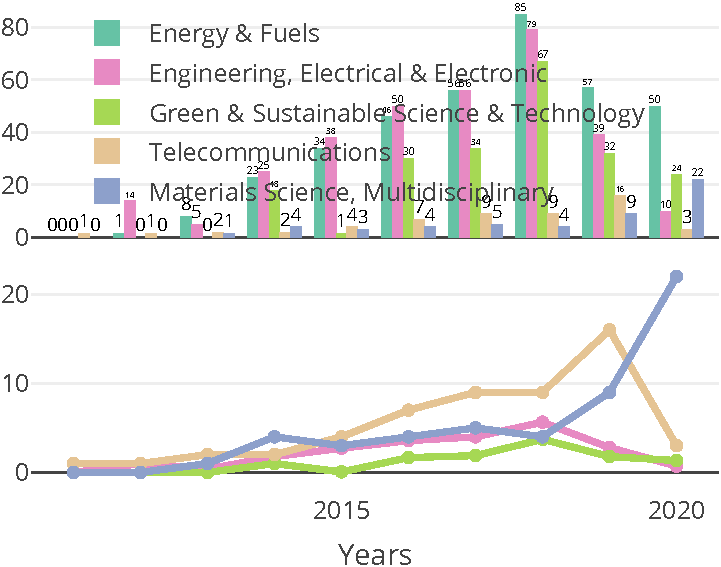
\includegraphics[width=1\linewidth]{01_bookdown_files/figure-latex/mohambarline-1} \caption{Absolute and relative growth of the most visible research areas in RE-related publications of Mohamed V University between 2011-2020}\label{fig:mohambarline}
\end{figure}

Similar to the other selected universities from the Northern Africa region \emph{Energy \& Fuels} has a strong presence also in the publications of \emph{Mohamed V Uni.}. Considering, there was no recorded renewable energy-related publication from \emph{Mohamed V Uni.} in 2011 and only 1 publication in 2012 in Web of Science databases, 2018 shows a strong contrast with 85 RE-related publications to the previous years. \emph{Electrical and Electronic Engineering} is following \emph{Energy and Fuels} closely in total RE-related publication from \emph{Mohamed V Uni.}.

Although, there are no recorded publications in \emph{Green and Sustainable Science \& Tech.} before 2014, it stays as the 3. most visible research area in the total numbers. In contrast to the other selected organisations so far one of the most visible research areas in the RE-related publications of \emph{Mohamed V University} is \emph{Telecommunications} and publications in \emph{Multidisciplinary Material Science} are also increasing since 2015. \emph{Multidisciplinary Material Science} is also the only research area that was increasing in numbers between 2019-2020 in the RE-related publications of \emph{Mohamed V University}.

\begin{figure}
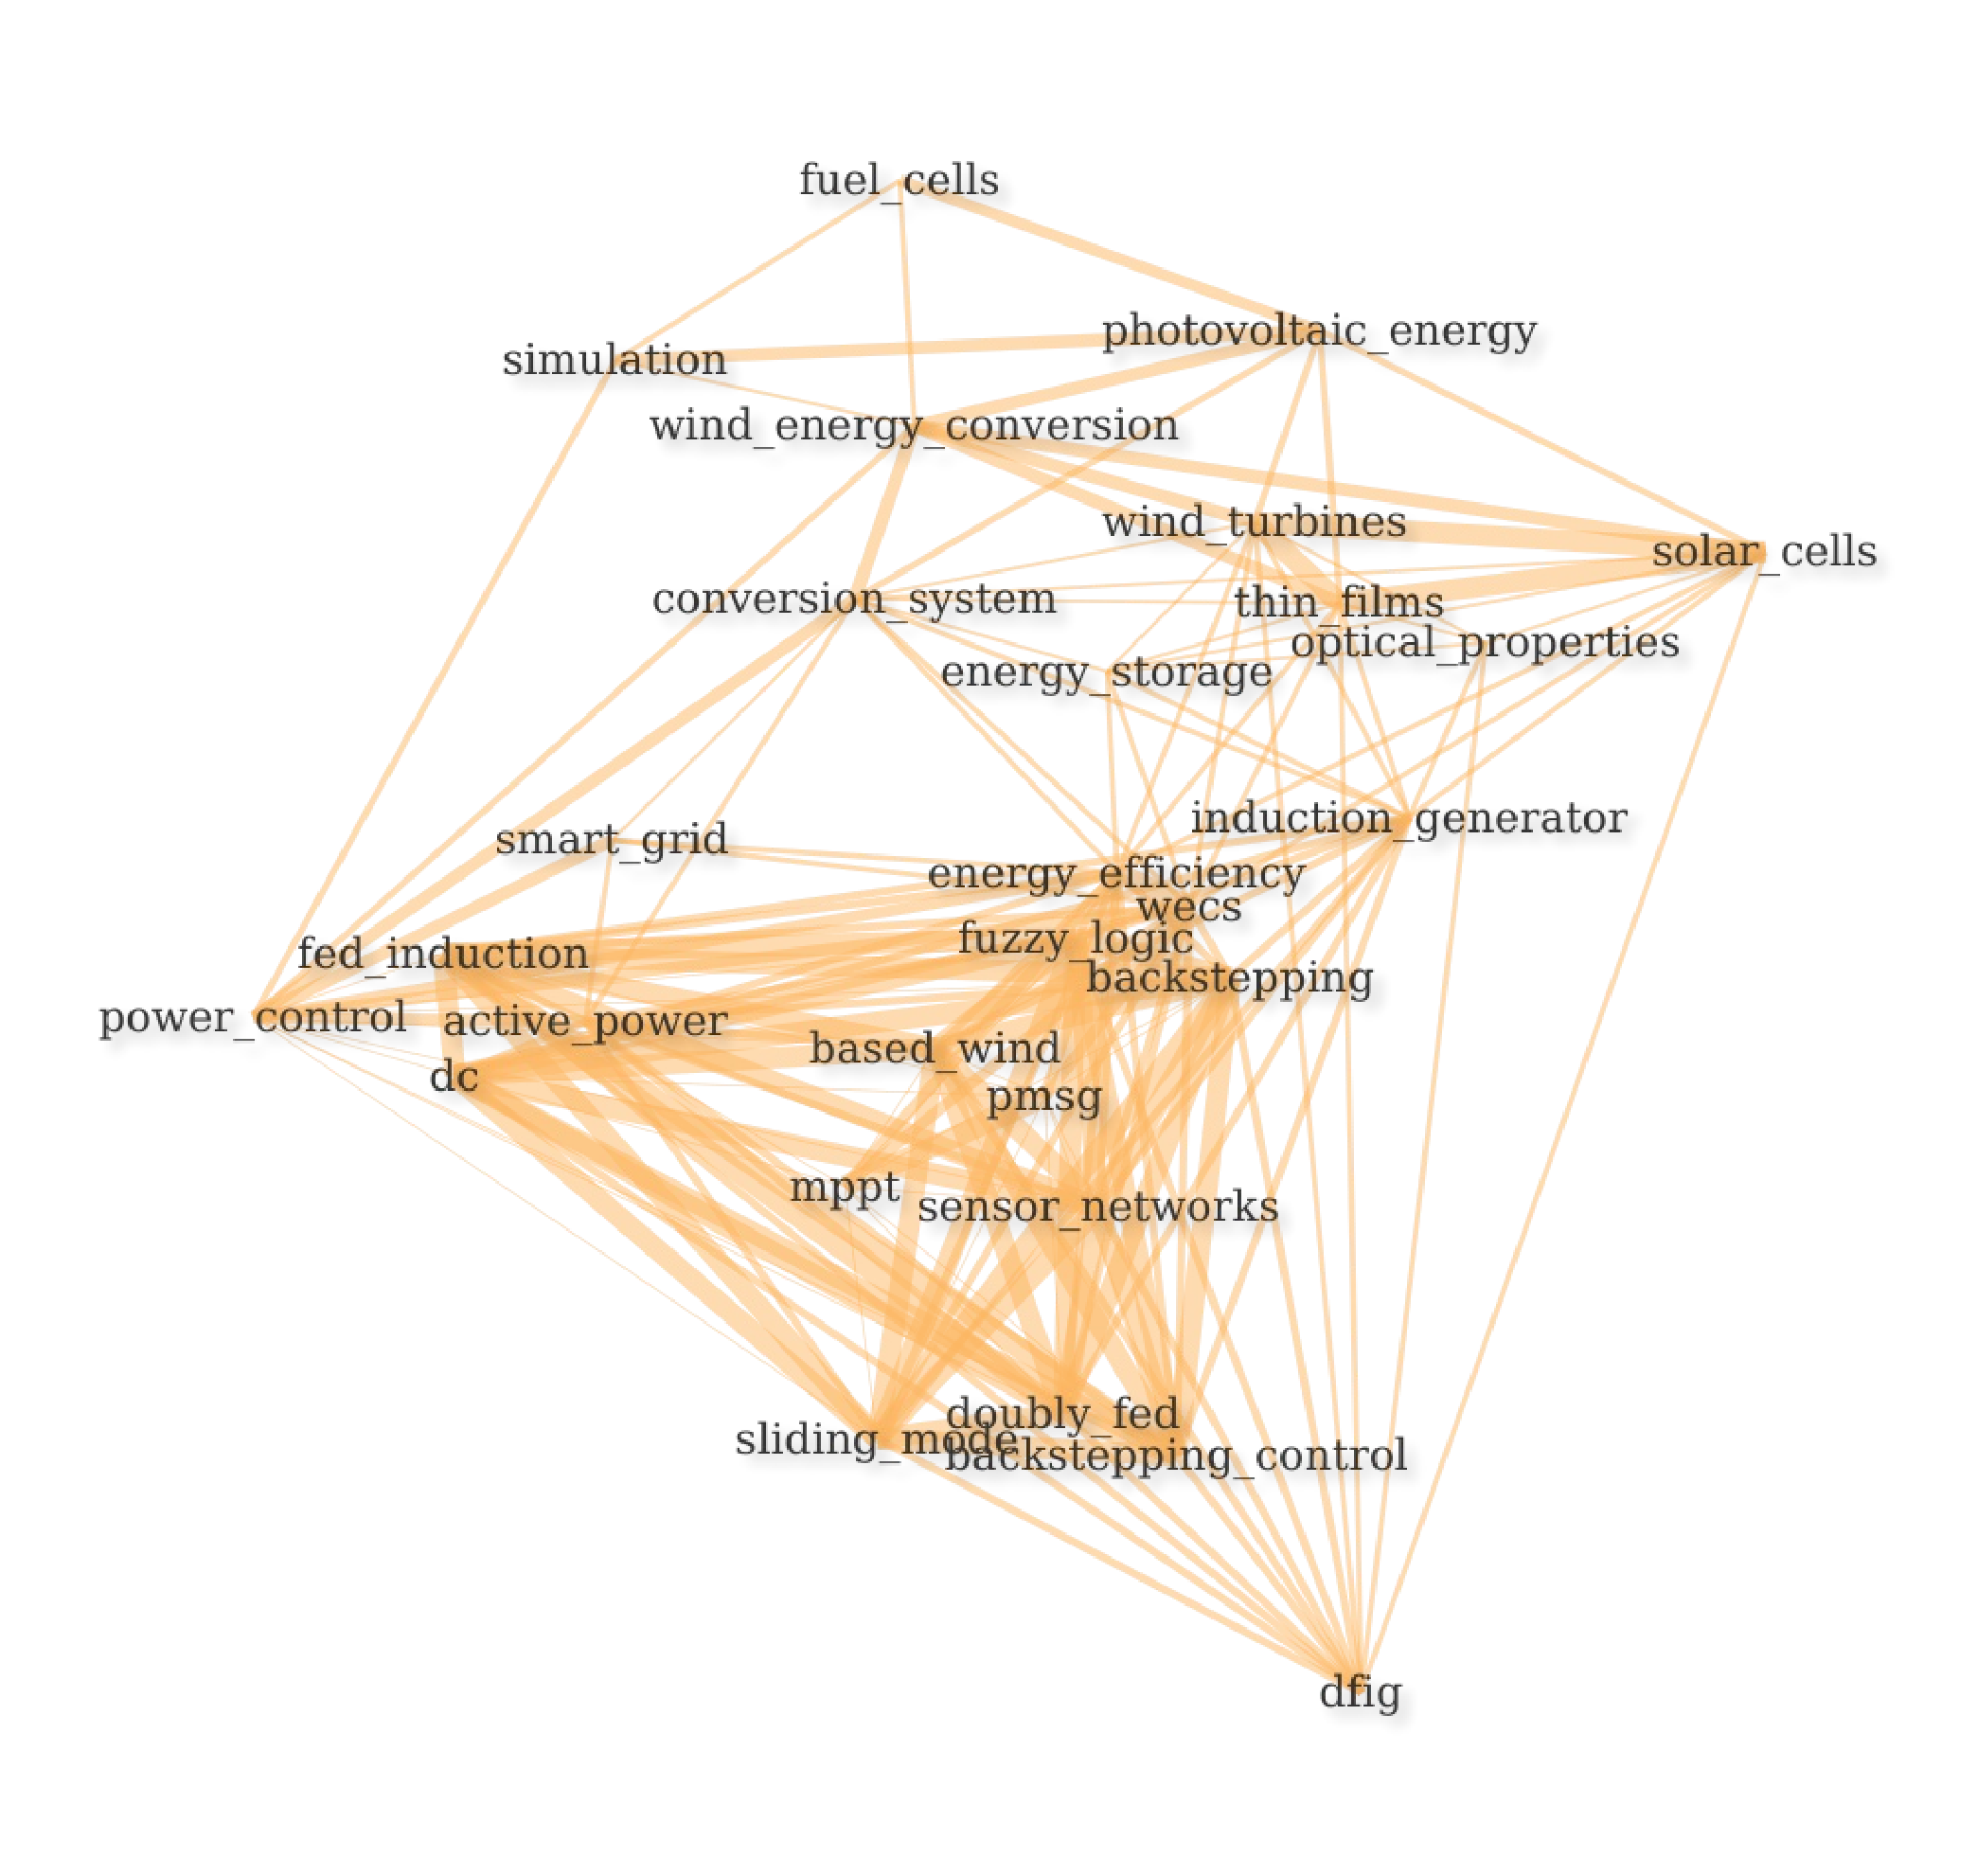
\includegraphics[width=1\linewidth]{01_bookdown_files/figure-latex/mohamngramnetwork-1} \caption{Keyword/keyword pair correlation network in RE-related publications of Mohammed V University}\label{fig:mohamngramnetwork}
\end{figure}

The keyword/keyword pair correlation network of \emph{Mohamed V University} also includes a number of solar energy and wind energy-related themes. Especially different types of conversion systems (wind energy conversion systems ) are reoccurring patterns in the RE-related publications of \emph{Mohamed V University}. In relation, hybrid energy approaches like \emph{doubly fed induction generator} (dfig) or backstepping control system that supports wind tribunes and photovoltaic systems (see \protect\hyperlink{ref-e.ahmed2012}{E. Ahmed and S. Yuvarajan} (\protect\hyperlink{ref-e.ahmed2012}{2012})) are emphasized. Also, dc-dc converter technologies like MPPT that aims to increase the efficiency of the photovoltaic systems are among the most visible keywords.

\hypertarget{western-africa-central-africa-eastern-africa}{%
\subsection{Western Africa, Central Africa, Eastern Africa}\label{western-africa-central-africa-eastern-africa}}

Western Africa, Central Africa and Eastern Africa are corresponding to a vast area of the African continent, however, on the organisations level number of RE-related publications are relatively fewer in comparison. Therefore, although on the country level those 3 regions will be analysed individually as in previous sub-chapters, on the organisations level; the table of the most visible organisations will include organisations from 3 selected countries of each region, and secondly, the organisation network will present organisations from all 3 regions on a single graph.

\hypertarget{western-africa}{%
\subsubsection{Western Africa}\label{western-africa}}

\begin{figure}
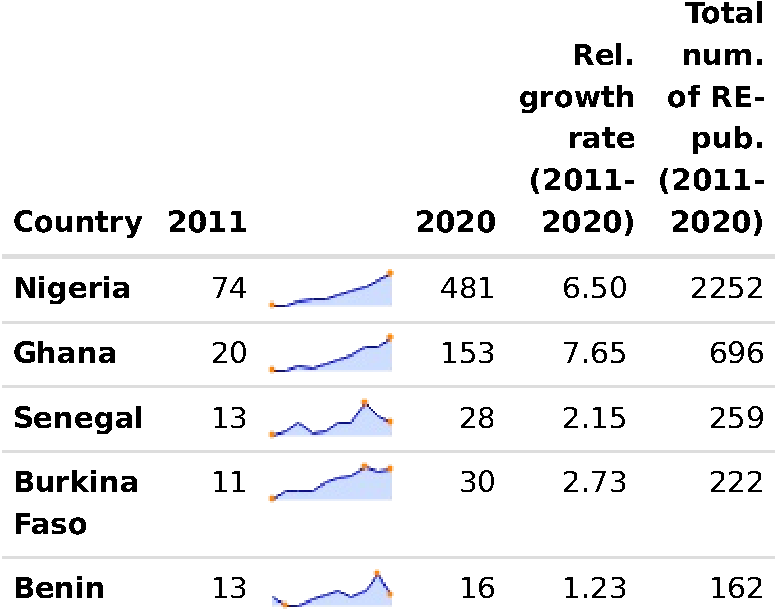
\includegraphics[width=1\linewidth]{01_bookdown_files/figure-latex/watable-1} \caption{RE-related publication output in Western African countries}\label{fig:watable}
\end{figure}

Western African countries Nigeria and Ghana have been increasing their RE-related publication
output in a consistent manner in the 10 years range (see table \ref{fig:watable}) without any stagnation. Although Nigeria's number of publications in 2011 was already relatively high in comparison (74 pub.), the number of publications in 2020 was \textasciitilde6.5 fold (481 pub.) of that. In a similar fashion, Ghana has increased its RE-related publication output from 20 in 2011 to 153 in 2020 which is an increment of a factor of \textasciitilde7.5.

Senegal, the third most visible country in the region shows a volatile progression with a sharp decline in the number of RE-related publications after 2018 from 48 yearly publications to 28. Burkina Faso is following Senegal with relatively less volatility and Benin's volatile numbers are expected since the total output of RE-related publications is fewer in comparison.

\begin{figure}

\includegraphics[width=1\linewidth]{01_bookdown_files/figure-latex/wanet-1} \caption{Co-publication network of Western African countries in RE-related publications between 2011-2020}\label{fig:wanet}
\end{figure}

Nigeria, the highest of the region in terms of the total number of RE-related publications, is also the centre of mass in the co-publication network of the Western African countries. It is the only Western African country with more than 25 co-publications with a Northern African country (Egypt, 26 co-pub). In a similar manner, together with Ghana, Nigeria is the only Western African country with more than 25 co-pub. with South Africa (277 pub.).

Ghana and Nigeria have a collaboration link with 40 RE-related co-publications between 2011-2020. However, the collaborations between the two most visible countries in the region with the other countries are relatively sparse. Côte d'Ivoire, Benin, Senegal, Burkina Faso and Mali are mostly engaged in their own cluster. The most visible international partner of that cluster is France. French academic organisations have co-published \textasciitilde400 papers with Western African countries between 2011-2020 and most of those have been carried out with the mentioned 5 countries. Germany is the second most visible EU-27 country in the region with \textasciitilde215 co-pub. with Western African countries followed by the Netherlands with 90 co-publications. Those 2 countries along with other EU-27 members like Sweden, Denmark and Italy are mostly engaged with the Nigeria-Ghana cluster.

Especially Nigeria has other international collaborations with relatively high output in terms of RE-related publications. A few examples of those are the collaborations with Malaysia (275 co-pub.), United Kingdom (215 co-pub.), United States (160 co-pub.) and China (40 co-publications).

\textbackslash begin\{figure\}
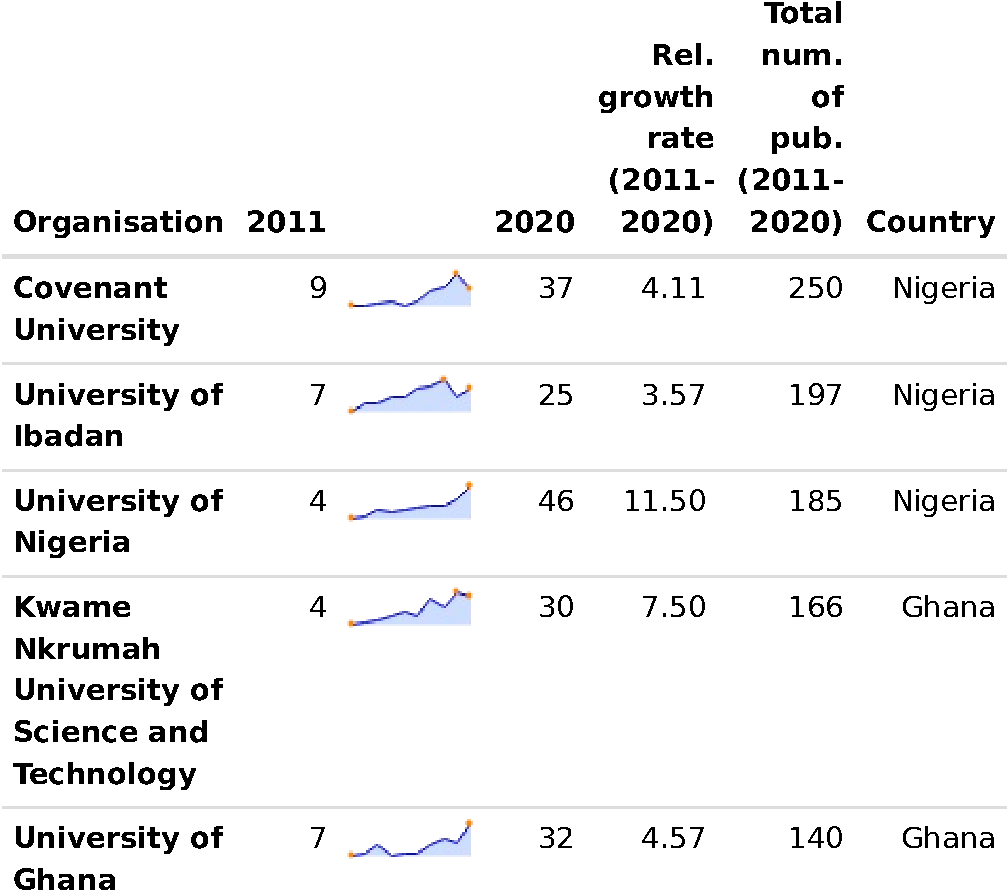
\includegraphics[width=0\linewidth]{01_bookdown_files/figure-latex/NigeriaGhanaSenegal-1}
All of the most visible 3 organisations in the selected West African countries Nigeria, Ghana, Senegal are from Nigeria. The number of RE-related publications of \emph{Covenant University}, the most visible organisation in the region, seems to be declining presumably because of the latency in document entries into WoS databases after 2019.

Other than \emph{Covenant University} total RE-related publication outputs of other most visible organisations in Western Africa are relatively close to each other. The \emph{University of Nigeria} has the highest relative growth rate of 11.5 (from 4 pub. in 2011 to 46 in 2020). Other than the \emph{University of Ibadan}, the other 3 organisations were also consistently increasing numbers of their RE-related publications despite two Ghanaian organisations showing slightly more volatile progress.

\hypertarget{central-africa}{%
\subsubsection{Central Africa}\label{central-africa}}

\begin{figure}
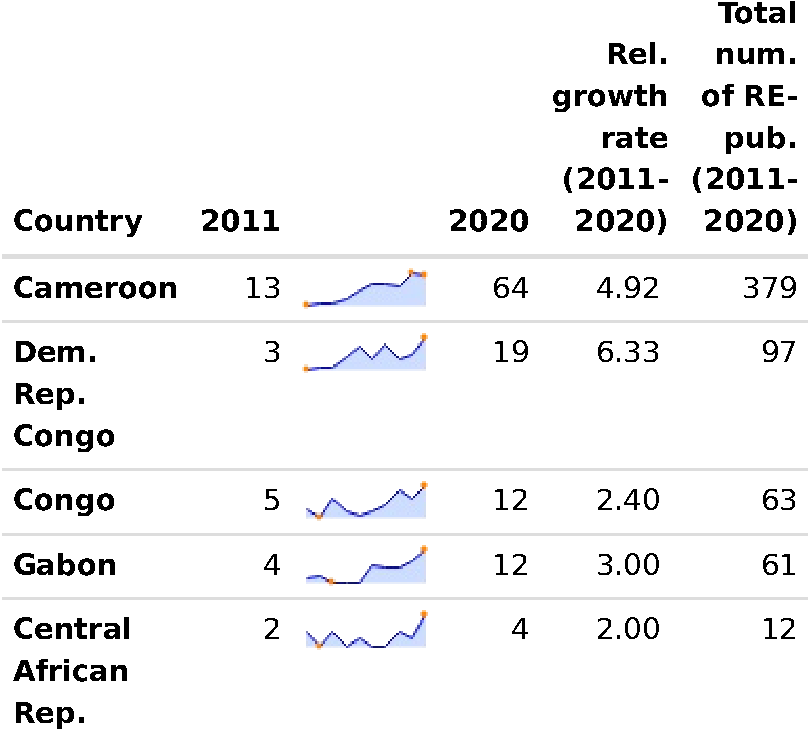
\includegraphics[width=1\linewidth]{01_bookdown_files/figure-latex/catable-1} \caption{RE-related publication output in Central African countries}\label{fig:catable}
\end{figure}

In the Central African region, the publication output in RE-related topics is relatively volatile. Cameroon shows a steady increment between 2011-2020 (see \ref{fig:catable}) with a total output of 379 RE-related publications in 10 years. Other than Cameroon, the total number of RE-related publications in other Central African countries stays under 100 in total between 2011-2020. Democratic Republic of Congo (DRC) is the second most visible country in the region; although DRC displays high volatility in number of yearly RE-related publications, 19 publications in 2020 is over 6 fold of the 3 publications back in 2011. Following 2 countries Republic of Congo and Gabon share similar numbers in general. Both countries have a total of \textasciitilde60 RE-related publications in the 10 years range and the closest following country is the Central African Republic with 12 RE-related publications in total.

\begin{figure}

\includegraphics[width=1\linewidth]{01_bookdown_files/figure-latex/canet-1} \caption{Co-publication network of Central African countries in RE-related publications between 2011-2020}\label{fig:canet}
\end{figure}

Although the publication output is not high in comparison with other regions, most of the publications in Central Africa are produced through intercontinental cooperation.\\
France is the most visible intercontinental collaborator in the co-publication network in Central Africa with 180 co-pub. in the region; 121 of those co-pub. have been published by collaboration with Cameroon. Belgium is following France with \textasciitilde90 co-pub. with Central African countries.

All of the visible international collaborators have published at least 25 RE-related co-publications with Cameroon. However, none of the Central African countries seems to have a co-publication link with another Central African country with an output of over 25 publications.

\textbackslash begin\{figure\}
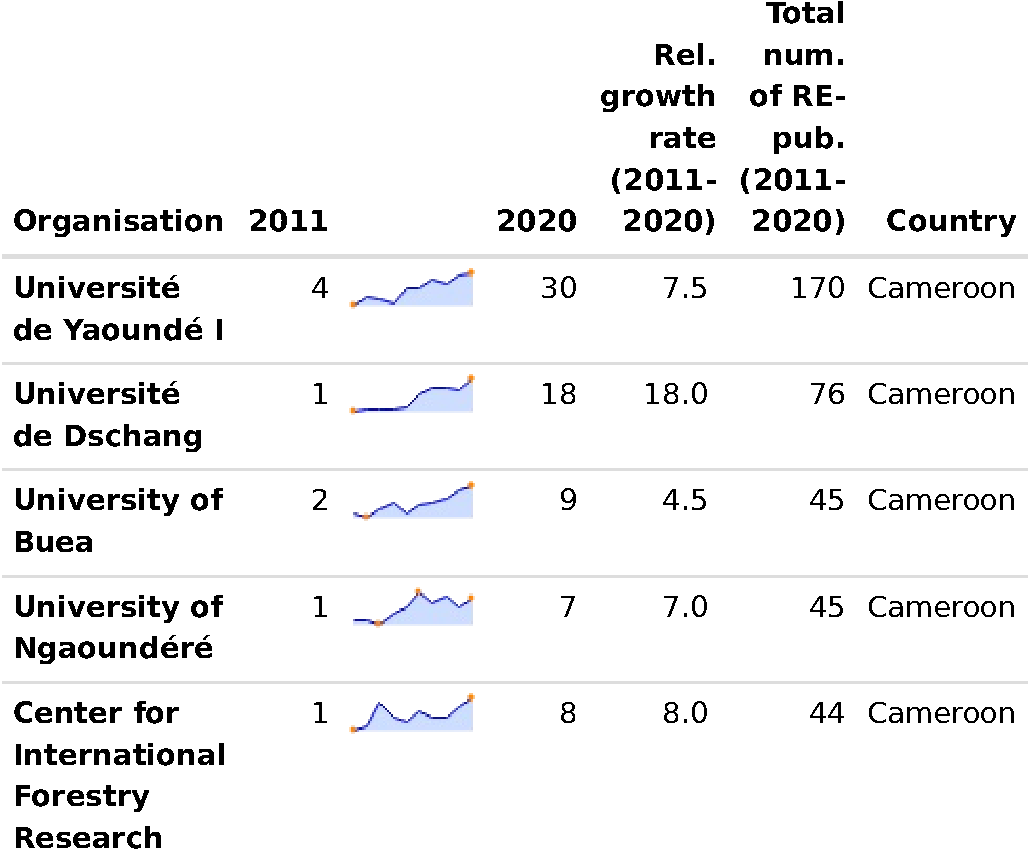
\includegraphics[width=0\linewidth]{01_bookdown_files/figure-latex/concamgab-1}
In the selected Central African countries Cameroon, Dem. Rep.~Congo, Gabon, all of the most visible 5 organisations in the region are from Cameroon with the most visible organisation being \emph{Université de Yaoundé I} with 170 RE-related publications in 2020. None of the organisations in the region has published more than 5 RE-related publications in 2011.

\emph{Université de Yaoundé I} is followed by \emph{Université de Dschang} which increased its 1 RE-related publication in 2011 to 18 in 2020 with a total of 76 RE-related publications in the 10-year range. The RE-related publication output of the following 3 organisations; \emph{University of Buea}, \emph{University of Ngaoundéré} and \emph{University of Douala} is still fewer than 10 yearly publications.

\hypertarget{eastern-africa}{%
\subsubsection{Eastern Africa}\label{eastern-africa}}

\begin{figure}
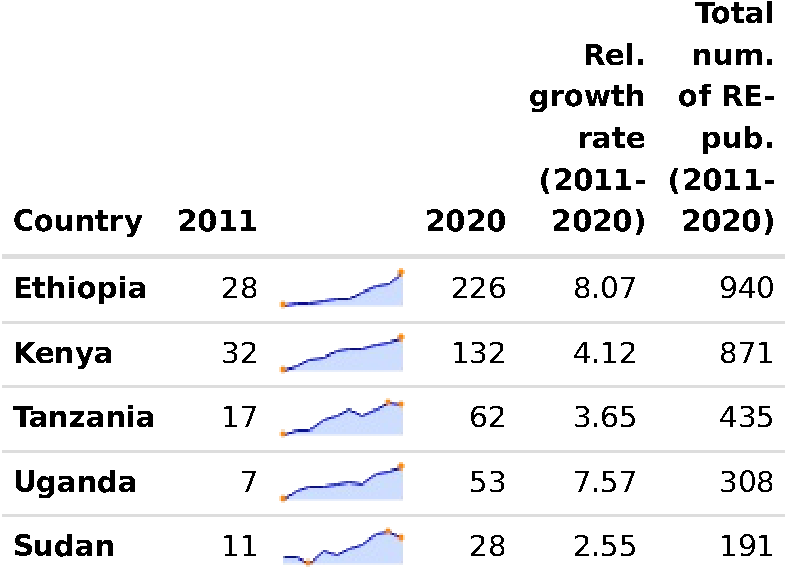
\includegraphics[width=1\linewidth]{01_bookdown_files/figure-latex/eatable-1} \caption{RE-related publication output in Eastern African countries}\label{fig:eatable}
\end{figure}

The most visible 5 Eastern African countries have been steadily increasing their numbers of RE-related publications. Ethiopia and Kenya are the most visible ones with 940 and 870 publications respectively. Ethiopia's number of publications in 2020 (226 pub.) is approximately 8 fold the number in 2011 (28).

The second most visible country in the region, Kenya's yearly output of RE-related publications was also linearly increasing after its already relatively high number in 2011 (32 publications). Tanzania follows Kenya with a fairly stable increment despite having approximately half of Kenya's total RE-related number of publications. Despite having 7 RE-related publications in 2011 Uganda is 4. most visible country in Eastern Africa after increasing its RE-related publication output \textasciitilde7.5 fold. Sudan is the 5. most visible country in Eastern Africa with \textasciitilde200 publications in total.

\begin{figure}

\includegraphics[width=1\linewidth]{01_bookdown_files/figure-latex/eanet-1} \caption{Co-publication network of Eastern African countries in RE-related publications between 2011-2020}\label{fig:eanet}
\end{figure}

The 4 most visible countries in Eastern Africa; Ethiopia, Kenya, Tanzania and Uganda are fairly interconnected in terms of RE-related co-publications with each other as well as with international collaborators. A number of EU-27 countries like France, Italy, Germany, Belgium, Sweden, Netherlands, Austria, Spain and Denmark are engaged in co-publications with Eastern African countries. Both Ethiopia and Kenya display a significant number of co-publications with Germany (72 and 134 pub. respectively). Although Ethiopia has the highest number of RE-related publications, Kenya seems to have more international co-publication links with relatively high co-publication output.

Several Eastern African countries have only international collaborations with more than 25 co-publications. That includes Madagascar with France as the only collaborator (63 co-pub.), Rwanda with United States (26 co-pub.), and Sudan with Saudi Arabia and China.

Other than EU countries the United States and the United Kingdom are also visible international partners engaged in RE-related research with Eastern African organisations. The United States has \textasciitilde500 (out of 2360 co-pub. with African countries) co-publications with the countries of Eastern Africa.

South Africa is the only African country from another region that has more than 25 RE-related co-publications with the Eastern African countries. South Africa's total RE-related co-publication output with the Eastern African countries between 2011-2020 is 199.

\textbackslash begin\{figure\}
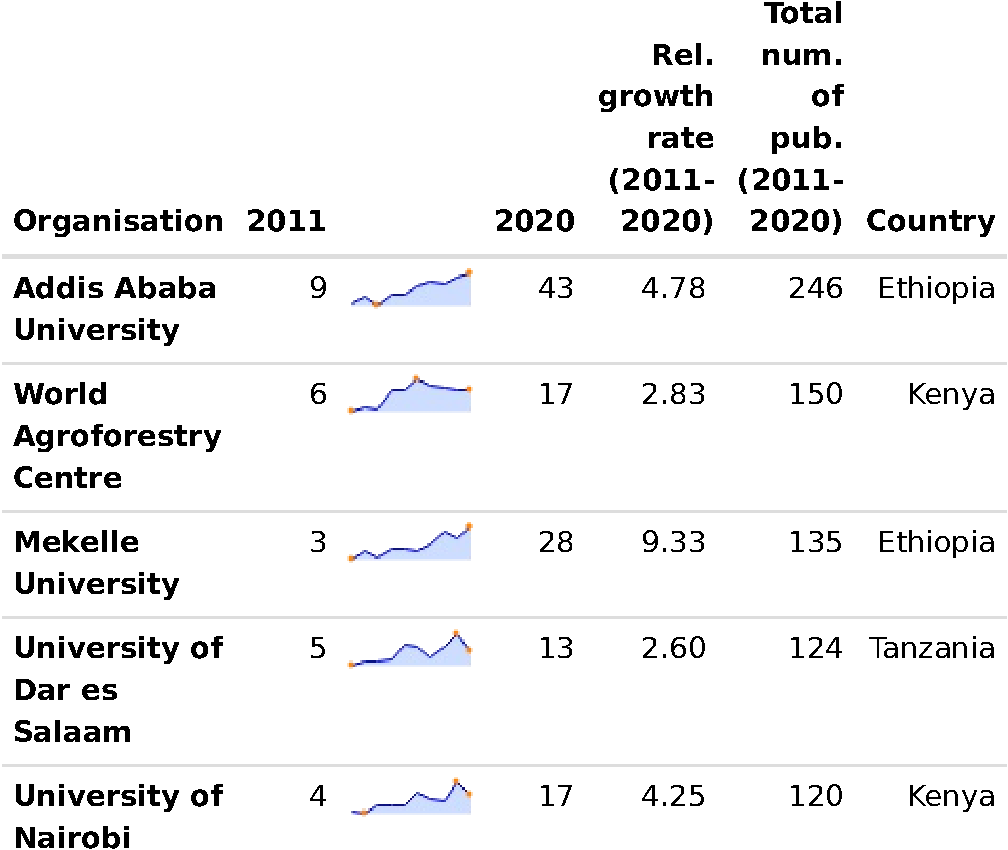
\includegraphics[width=0\linewidth]{01_bookdown_files/figure-latex/ethkentan-1}

Most visible countries from the selected countries in Eastern Africa, namely Ethiopia, Kenya Tanzania are diverse. \emph{Addis Ababa University} from Ethiopia is the most visible one with 246 RE-related publications between 2011-2020. The number of publications of \emph{Addis Ababa University} has been increasing steadily since 2013.

Although \emph{World Agroforestry Centre} operates in different countries, the main location of the institution is registered as Kenya. \emph{World Agroforestry Centre} is the second most visible organisation in the selected East African countries Ethiopia, Kenya, Tanzania with a total number of 150 publications between 2011-2020. However, the yearly number of publications are declining since 2016.

\emph{Mekelle University} of Ethiopia is the third most visible organisation with steady growth in the number of RE-related publications and \emph{University of Dar es Salaam} is the only organisation from Tanzania in the 5 most visible countries in the selected countries of East Africa followed by the \emph{University of Nairobi} of Kenya.

\hypertarget{selected-institutions-and-institutional-co-publication-network}{%
\subsubsection{Selected Institutions and Institutional Co-publication Network}\label{selected-institutions-and-institutional-co-publication-network}}

\begin{figure}
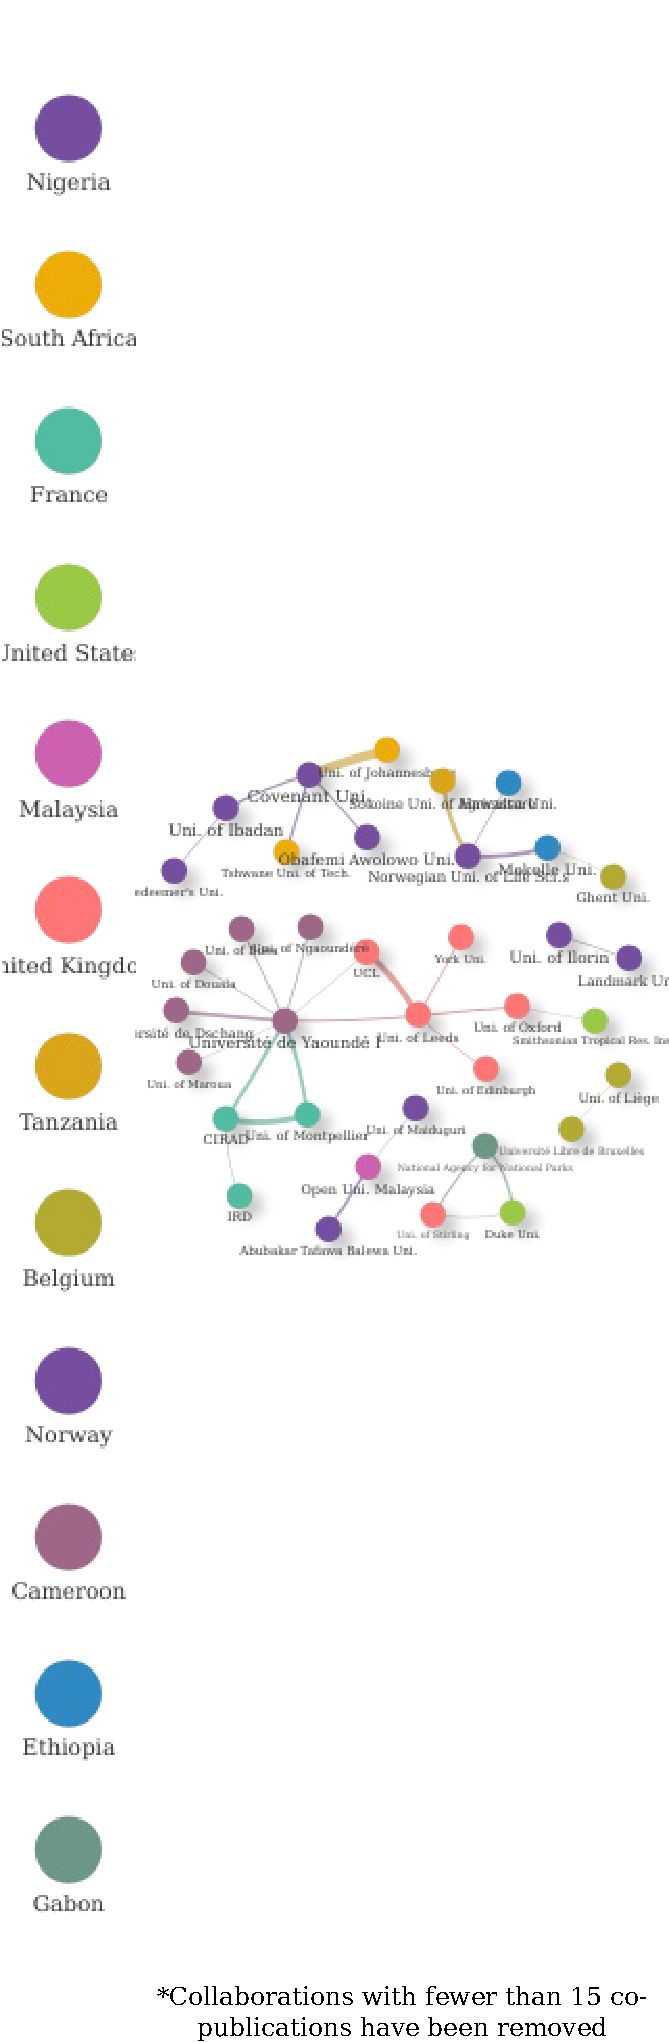
\includegraphics[width=1\linewidth]{01_bookdown_files/figure-latex/wacaeaorgnet-1} \caption{Co-publication network of Western, Central, Eastern African organisations in RE-related publications between 2011-2020}\label{fig:wacaeaorgnet}
\end{figure}

Collective organisation network of Western, Central and Eastern African regions displays a couple of interconnected co-publication clusters. Organisations from Cameroon are one of the most visible clusters where \emph{Université Yaoundé I} stands as a central connection node. \emph{Université de Dschang}, \emph{Uni. of Buea} and \emph{Université De Ngaoundéré} are the other academic organisations from Cameroon which co-published visible amount of RE-related publications with \emph{Université Yaoundé I} (22, 17 and 17 co-publications respectively). The network of Cameroonian universities is connected to French and British organisations with a visible amount of publications. On the French side \emph{Uni. of Montpellier} and \emph{CIRAD} both have 22 co-publications with \emph{Université Yaoundé I} and on the other side \emph{Uni. of Leeds} has a collaboration of 18 RE-related co-publications with \emph{Université Yaoundé I} where other British academic organisations like \emph{UCL}, \emph{Uni. of Oxford} and \emph{York Uni.} are also present in a number of those co-publications.

Nigerian Universities form another visible cluster in the co-publication network whereas \emph{Covenant University} plays a central role. \emph{Uni. of Ibadan} and \emph{Obafemi Awolowo Uni.} both have \textasciitilde20 co-publications with \emph{Covenant University}. Also, \emph{Covenant University}'s collaborations with South African institutions are in the most visible co-pub. connections in the region, \emph{University of Johannesburg} has co-published 34 RE-related publications with \emph{Covenant University}.

Other visible collaborations are \emph{Norwegian Uni. of Life Sciences}' co-publications with Tanzania's \emph{Sokoine Uni. of Agriculture} (24 co-pub.) and with Ethiopia's \emph{Mekelle University} (22 co-pub.).

\hypertarget{covenant-university-nigeria}{%
\paragraph{Covenant University (Nigeria)}\label{covenant-university-nigeria}}

\begin{figure}
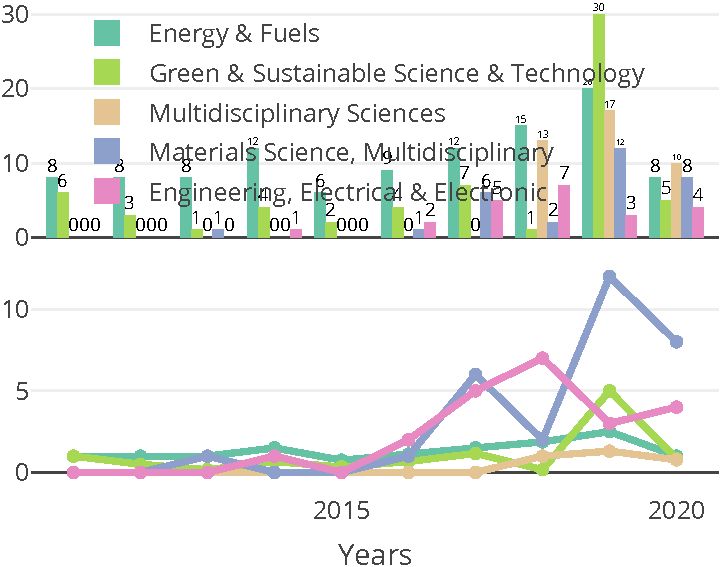
\includegraphics[width=1\linewidth]{01_bookdown_files/figure-latex/covenbarline-1} \caption{Absolute and relative growth of the most visible research areas in RE-related publications of Covenant University between 2011-2020}\label{fig:covenbarline}
\end{figure}

The most visible research areas are \emph{Energy \& Fuels} and \emph{Green \& Sustainable Science \& Technology} respectively in RE-related publications of \emph{Covenant University}. 2019 is in terms of RE-related publications a peak point for \emph{Covenant University}, the 2 two most visible areas include 20 and 30 publications respectively in this year.

None of the last three categories \emph{Multidisciplinary Sciences},\footnote{Web of Science uses the category Multidisciplinary Sciences to define scientific journals that contain a large number of disciplines.} \emph{Material Science} and \emph{Electrical \& Electronic Engineering} had more than 1 yearly RE-related publication in \emph{Covenant University} until 2016. However, although there weren't any publications in \emph{Multidisciplinary Sciences} until 2017, it has become one of the most visible categories in \emph{Covenant University's} RE-related publications with yearly over 10 publications.

\begin{figure}
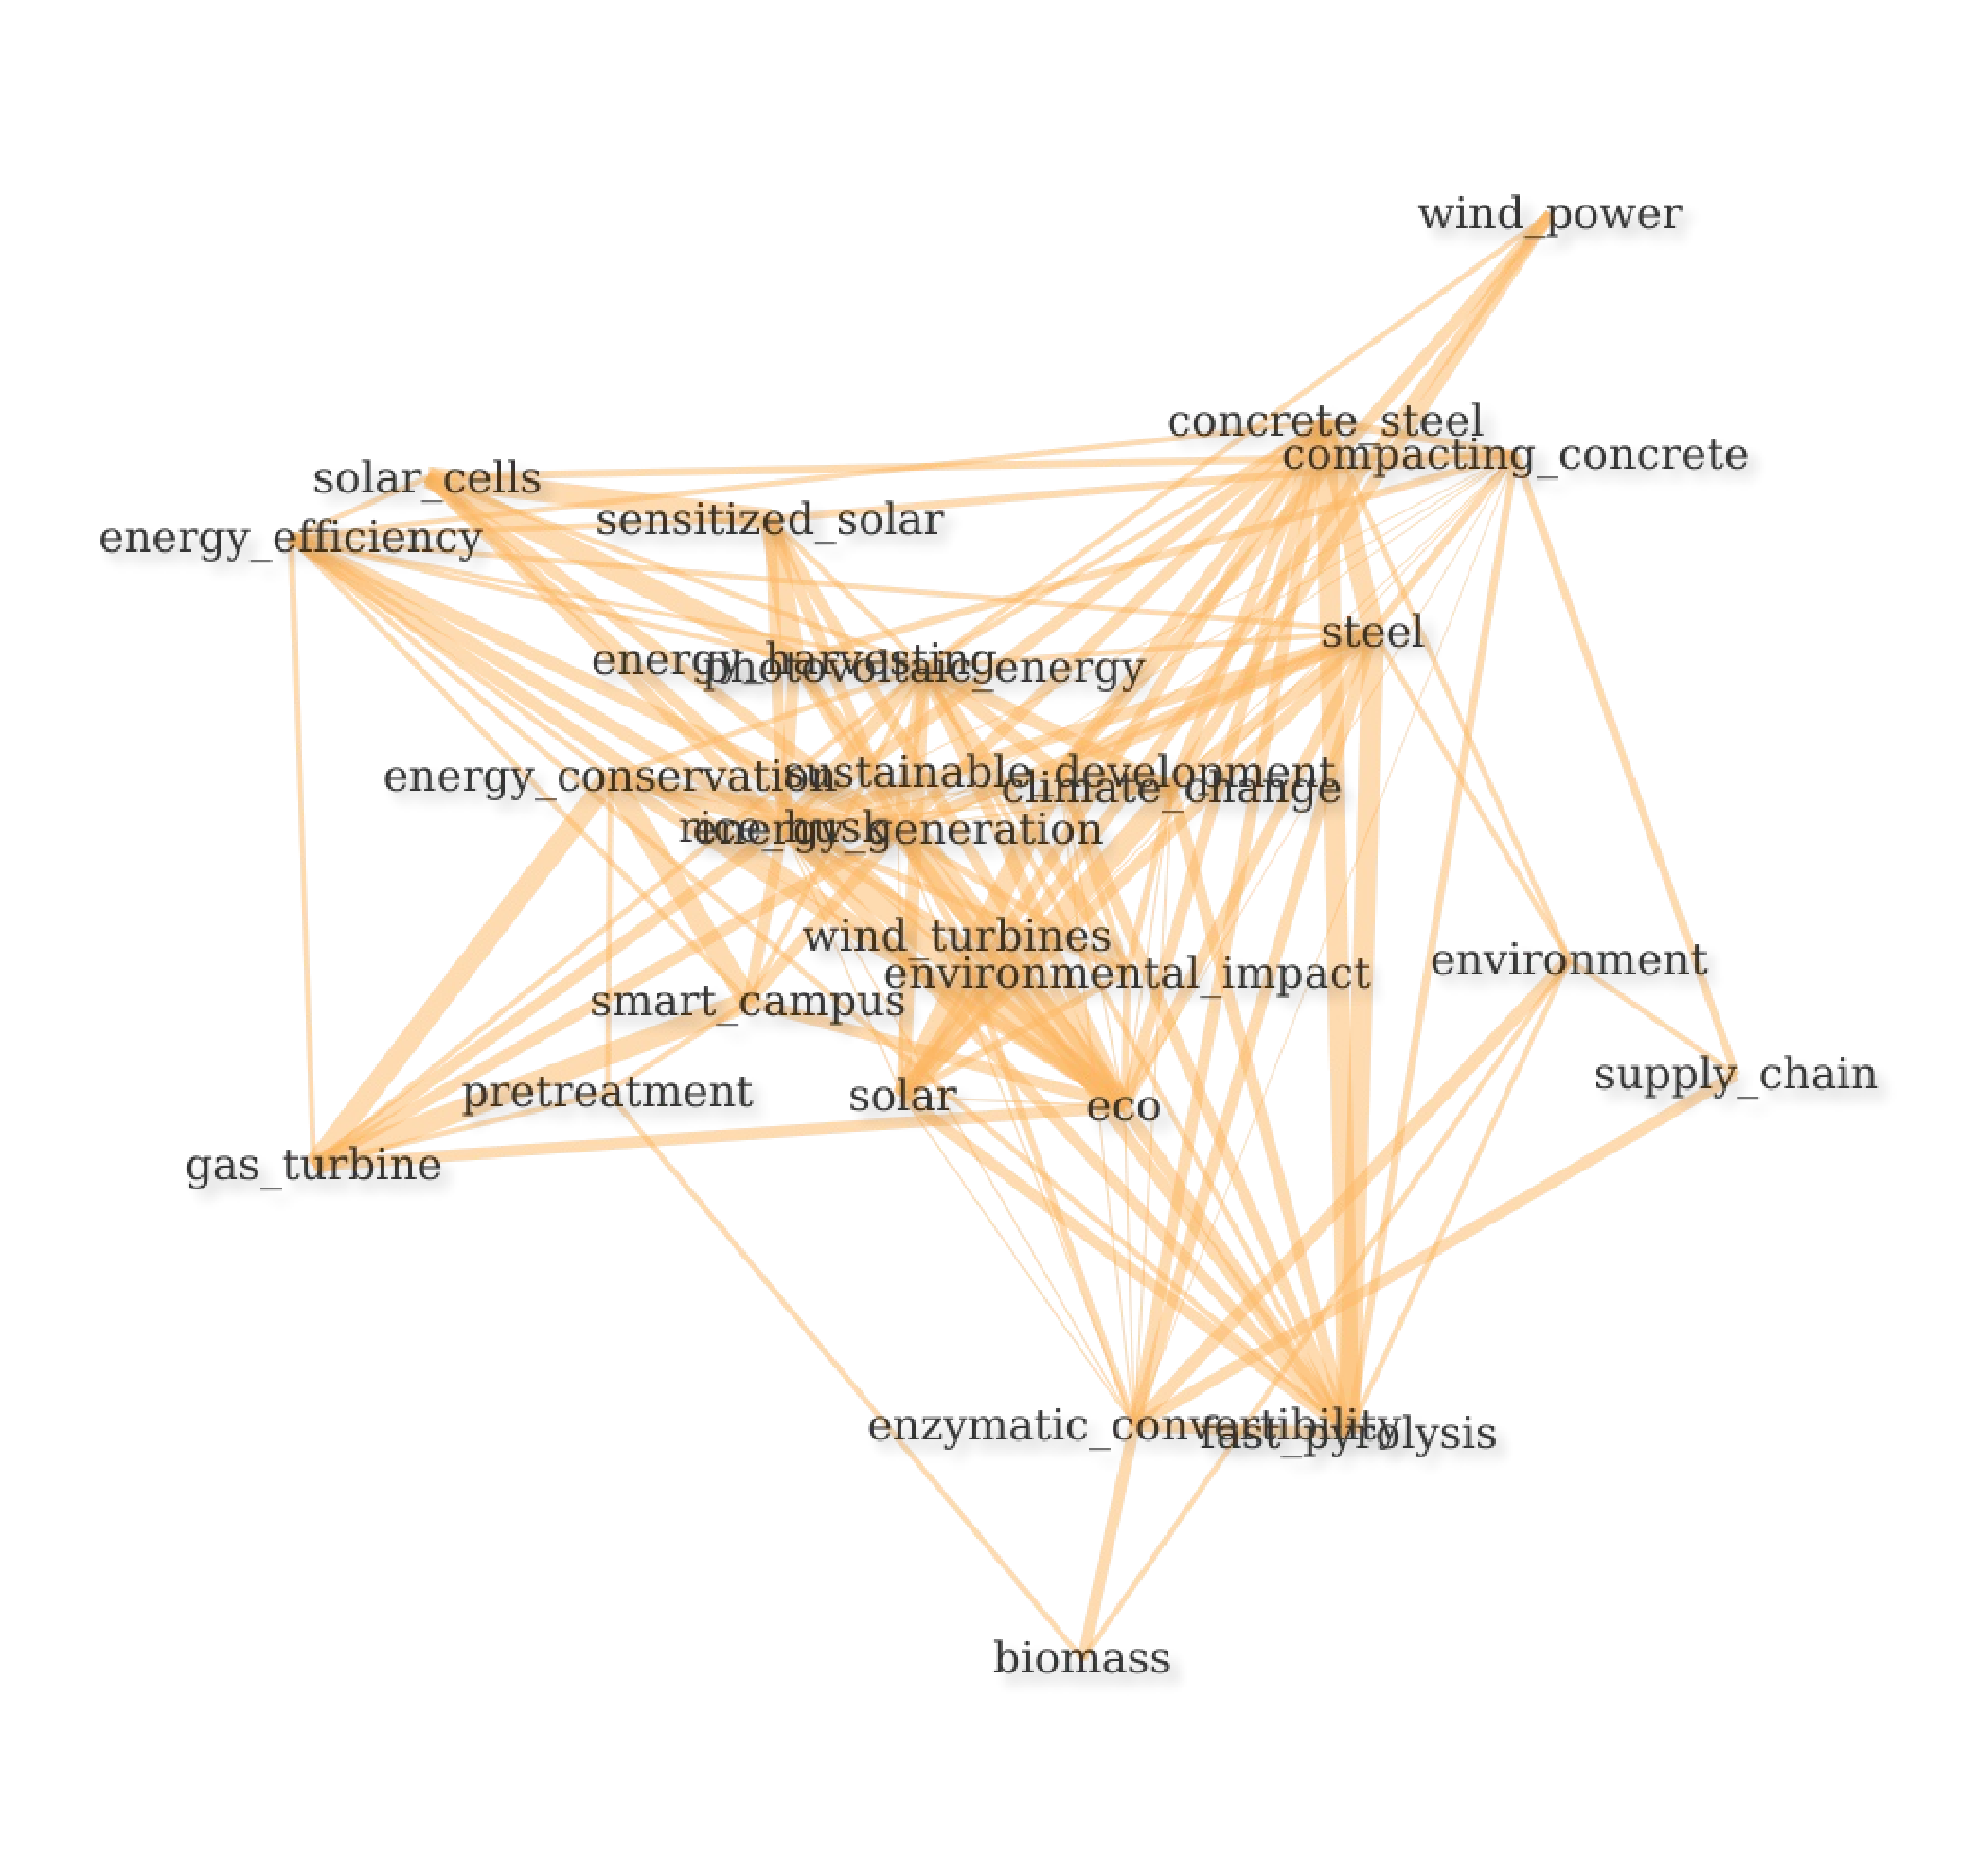
\includegraphics[width=1\linewidth]{01_bookdown_files/figure-latex/covenngramnetwork-1} \caption{Keyword/keyword pair correlation network in RE-related publications of Covenant University}\label{fig:covenngramnetwork}
\end{figure}

Similar to the research areas keyword/keyword pair correlation network of \emph{Covenant University} also includes some differing elements. Along with a heavy emphasis on solar and wind energy-related topics, one of the central keyword pairs indicates the research on using rice husk, a byproduct of rice growing, as a biomass fuel. Presumably several mentions of concrete and steel, firstly, relates to the production of those materials with renewable energy, and secondly, as \emph{compacting\_concrete} indicates research on producing environment-friendly forms of (self-) compacting concrete which has more than one benefit for sustainable development (further reading: \protect\hyperlink{ref-long2015}{Long, Gao, and Xie} (\protect\hyperlink{ref-long2015}{2015}) and \protect\hyperlink{ref-gupta2021}{Gupta, Siddique, and Belarbi} (\protect\hyperlink{ref-gupta2021}{2021})).

Also, keyword pairs like \emph{fast\_pyrolysis} and \emph{enzymatic\_convertibility} indicate a relatively high number of biomass related studies.

\hypertarget{university-of-nigeria}{%
\paragraph{University of Nigeria}\label{university-of-nigeria}}

\begin{figure}
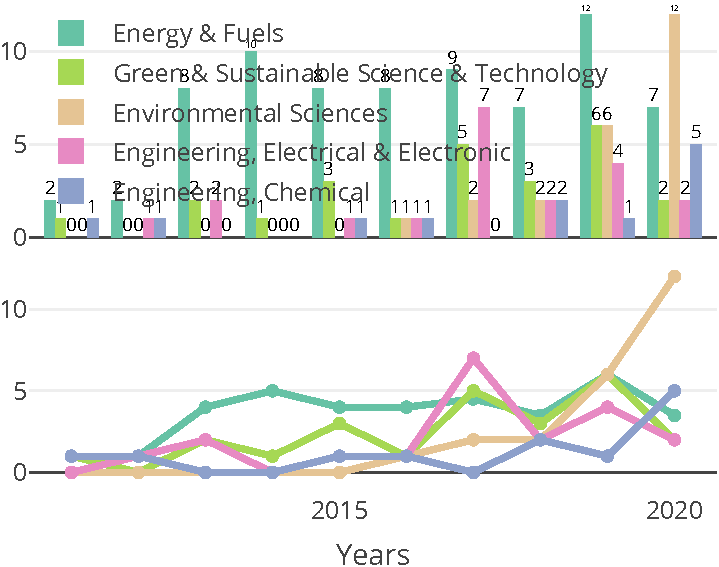
\includegraphics[width=1\linewidth]{01_bookdown_files/figure-latex/uninibarline-1} \caption{Absolute and relative growth of the most visible research areas in RE-related publications of University of Nigeria between 2011-2020}\label{fig:uninibarline}
\end{figure}

The \emph{University of Nigeria} also starts with a fairly low number of publications in the now trending research areas. Until 2013 none of the most visible 5 research areas includes a yearly output of over 2 RE-related publications. Energy \& Fuels spikes in the later years followed by Green \& Sustainable Science \& Technology. However, while the two most visible areas are stagnating or declining Environmental Sciences starts to grow in numbers and become together with Chemical Engineering the only areas still rising in 2020.

\begin{figure}
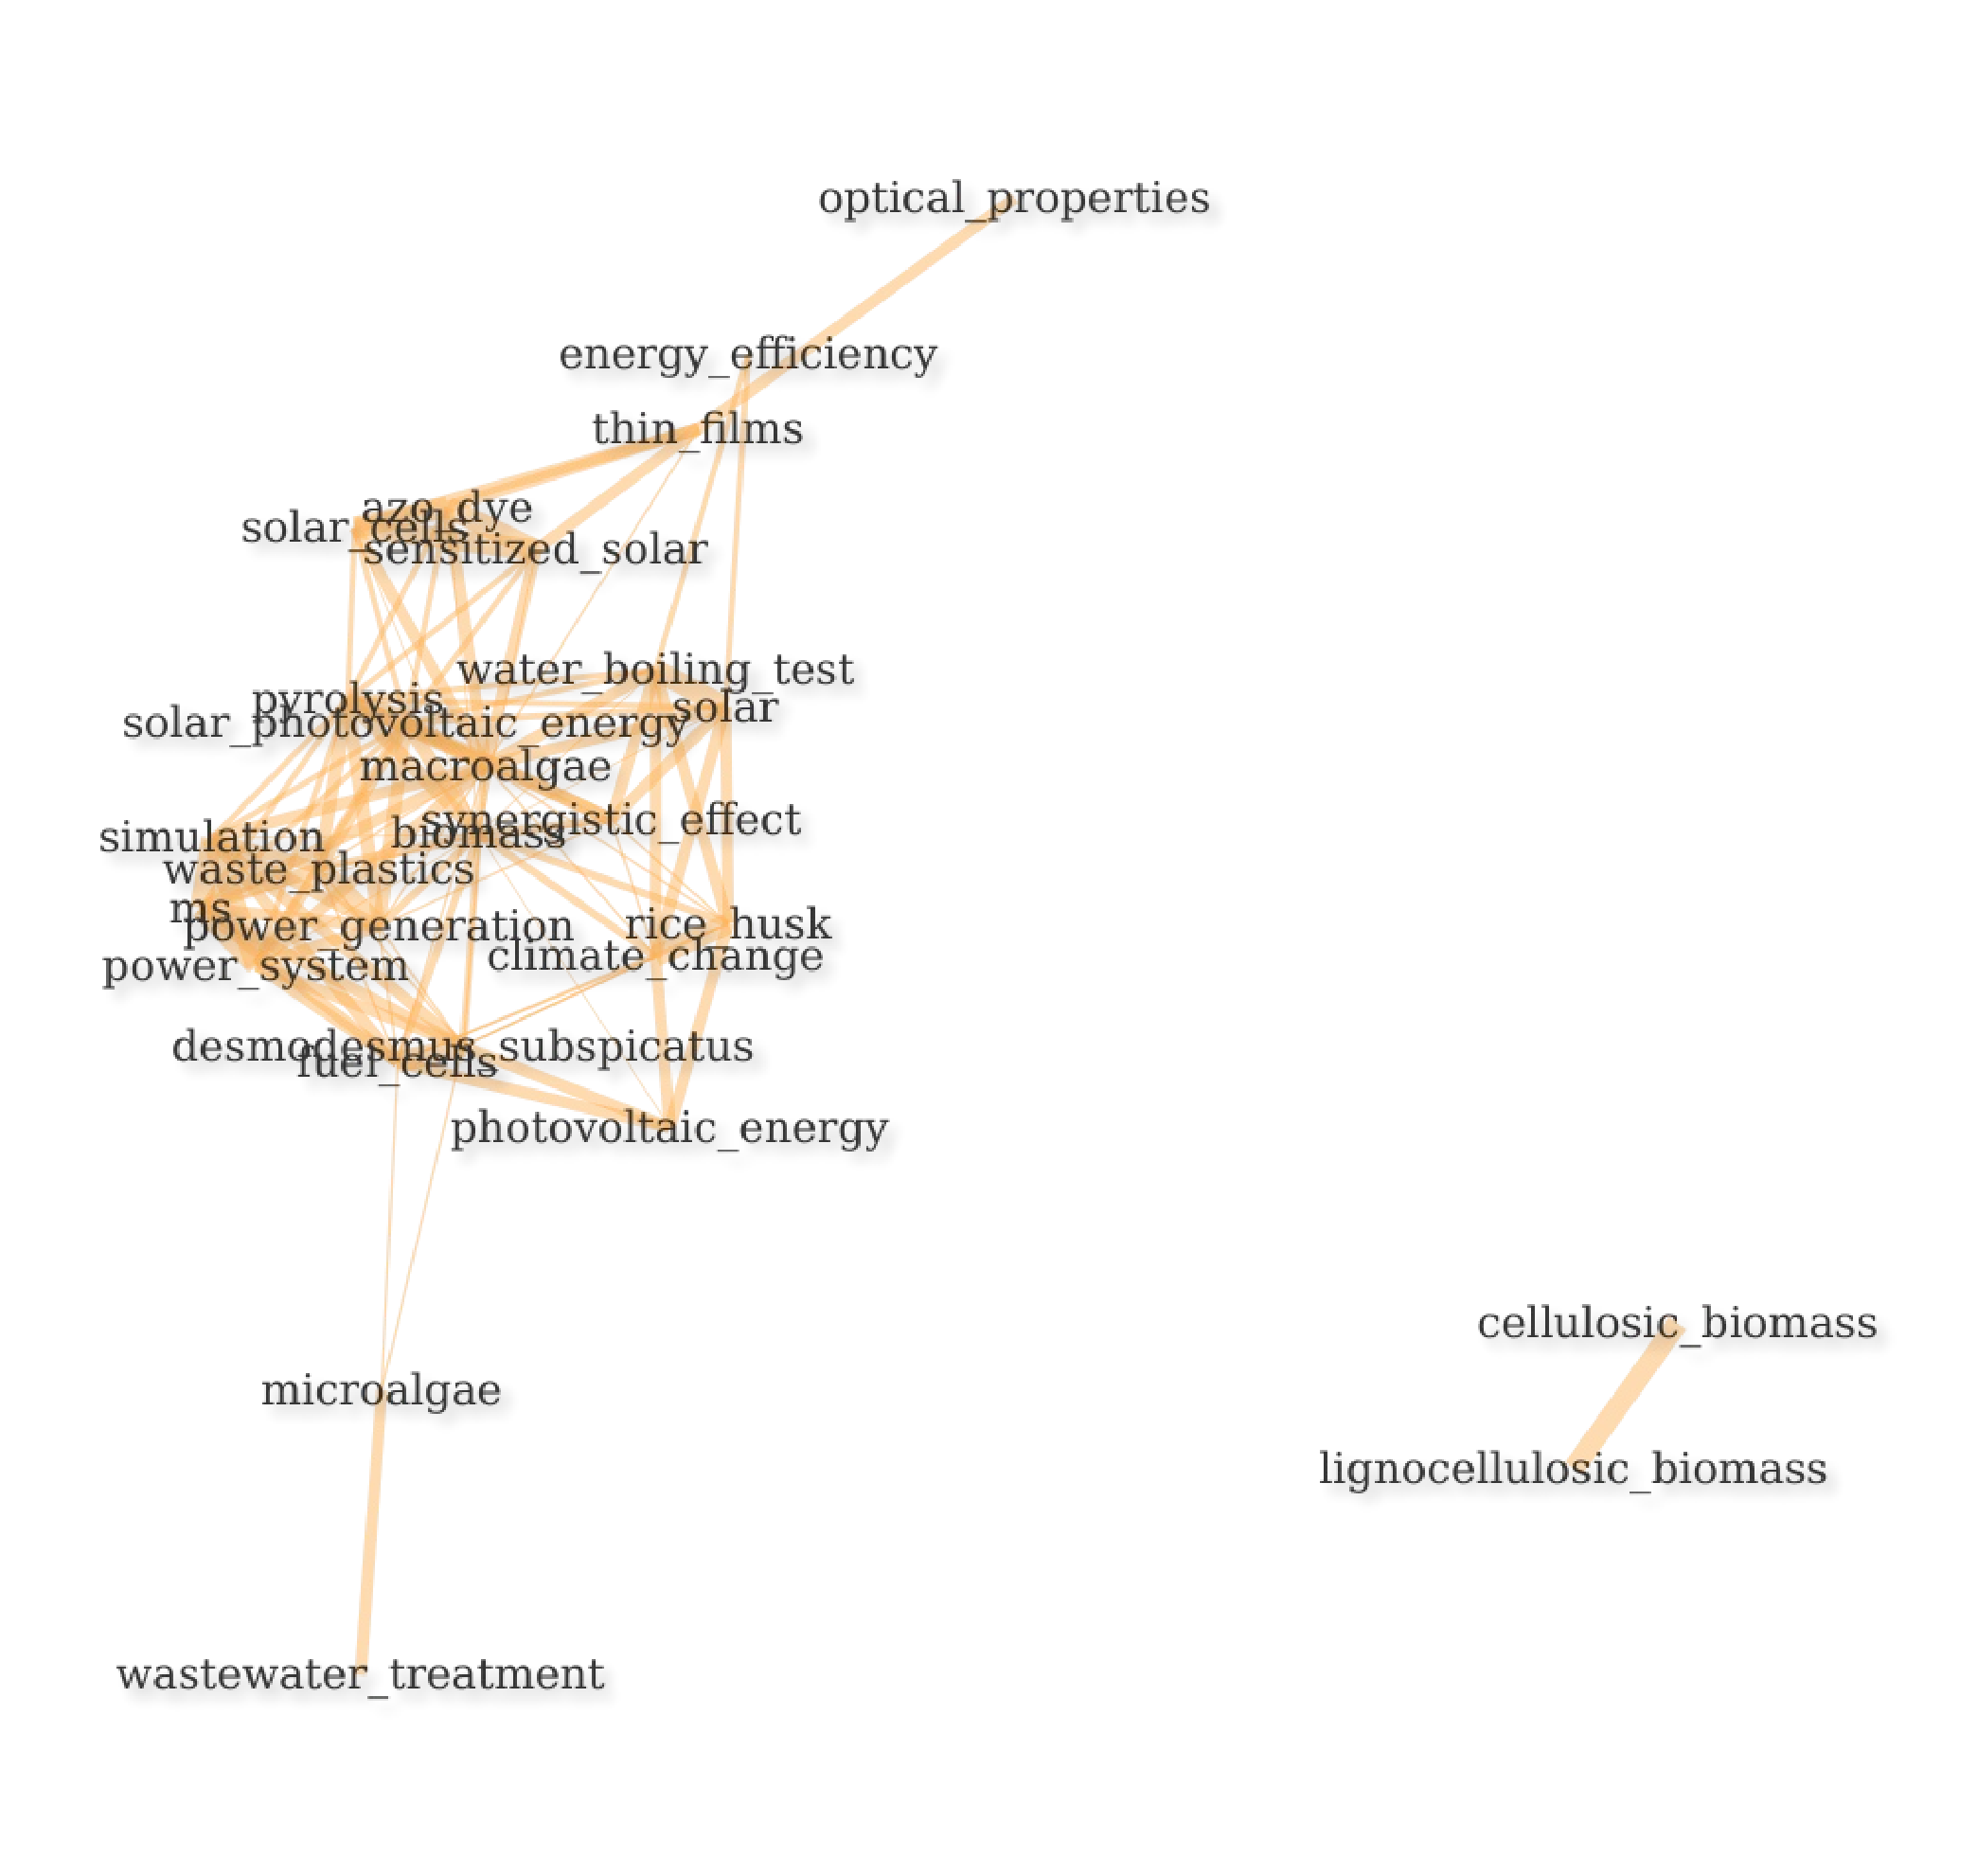
\includegraphics[width=1\linewidth]{01_bookdown_files/figure-latex/uniningramnetwork-1} \caption{Keyword/keyword pair correlation network in RE-related publications of University of Nigeria}\label{fig:uniningramnetwork}
\end{figure}

The \emph{University of Nigeria} also includes some unique keyword pairs. Along with the usual emphasized renewable energy forms like solar and wind energy RE-related publications of the \emph{University of Nigeria} puts high emphasis on biomass related topics. In conjunction, also micro- and macroalgae are often reoccurring keywords in the RE-related publications of \emph{University of Nigeria}, these are recently discussed in the renewable energy-related areas because of their potential to be used as biofuel (see \protect\hyperlink{ref-khan2018}{Khan, Shin, and Kim} (\protect\hyperlink{ref-khan2018}{2018})). Also, a couple of keywords pairs indicate wastewater treatment, removal and recycling of waste plastics are also visible topics in the publications of \emph{University of Nigeria}.

\hypertarget{universituxe9-de-yaounduxe9-i-cameroon}{%
\paragraph{Université de Yaoundé I (Cameroon)}\label{universituxe9-de-yaounduxe9-i-cameroon}}

\begin{figure}
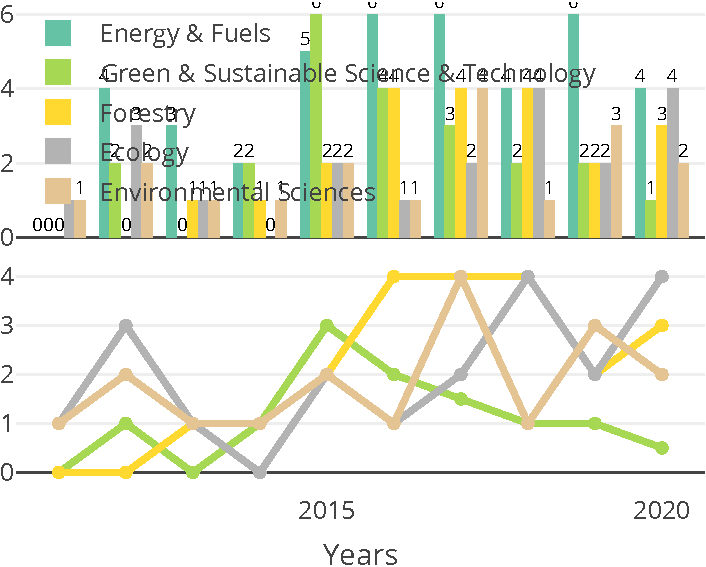
\includegraphics[width=1\linewidth]{01_bookdown_files/figure-latex/yaounbarline-1} \caption{Absolute and relative growth of the most visible research areas in RE-related publications of Université de Yaoundé I between 2011-2020}\label{fig:yaounbarline}
\end{figure}

Most visible research areas in the RE-related publications of \emph{Université de Yaoundé I} are relatively uniformly distributed. Energy \& Fuels is the most visible one followed by Green \& Sustainable Science \& Technology. However, starting with 2015 Forestry, Ecology, and Environmental Sciences gain visibility. Especially the visibility of the research area Forestry is unique to \emph{Université de Yaoundé I} among the most visible organisations in Africa.

\begin{figure}
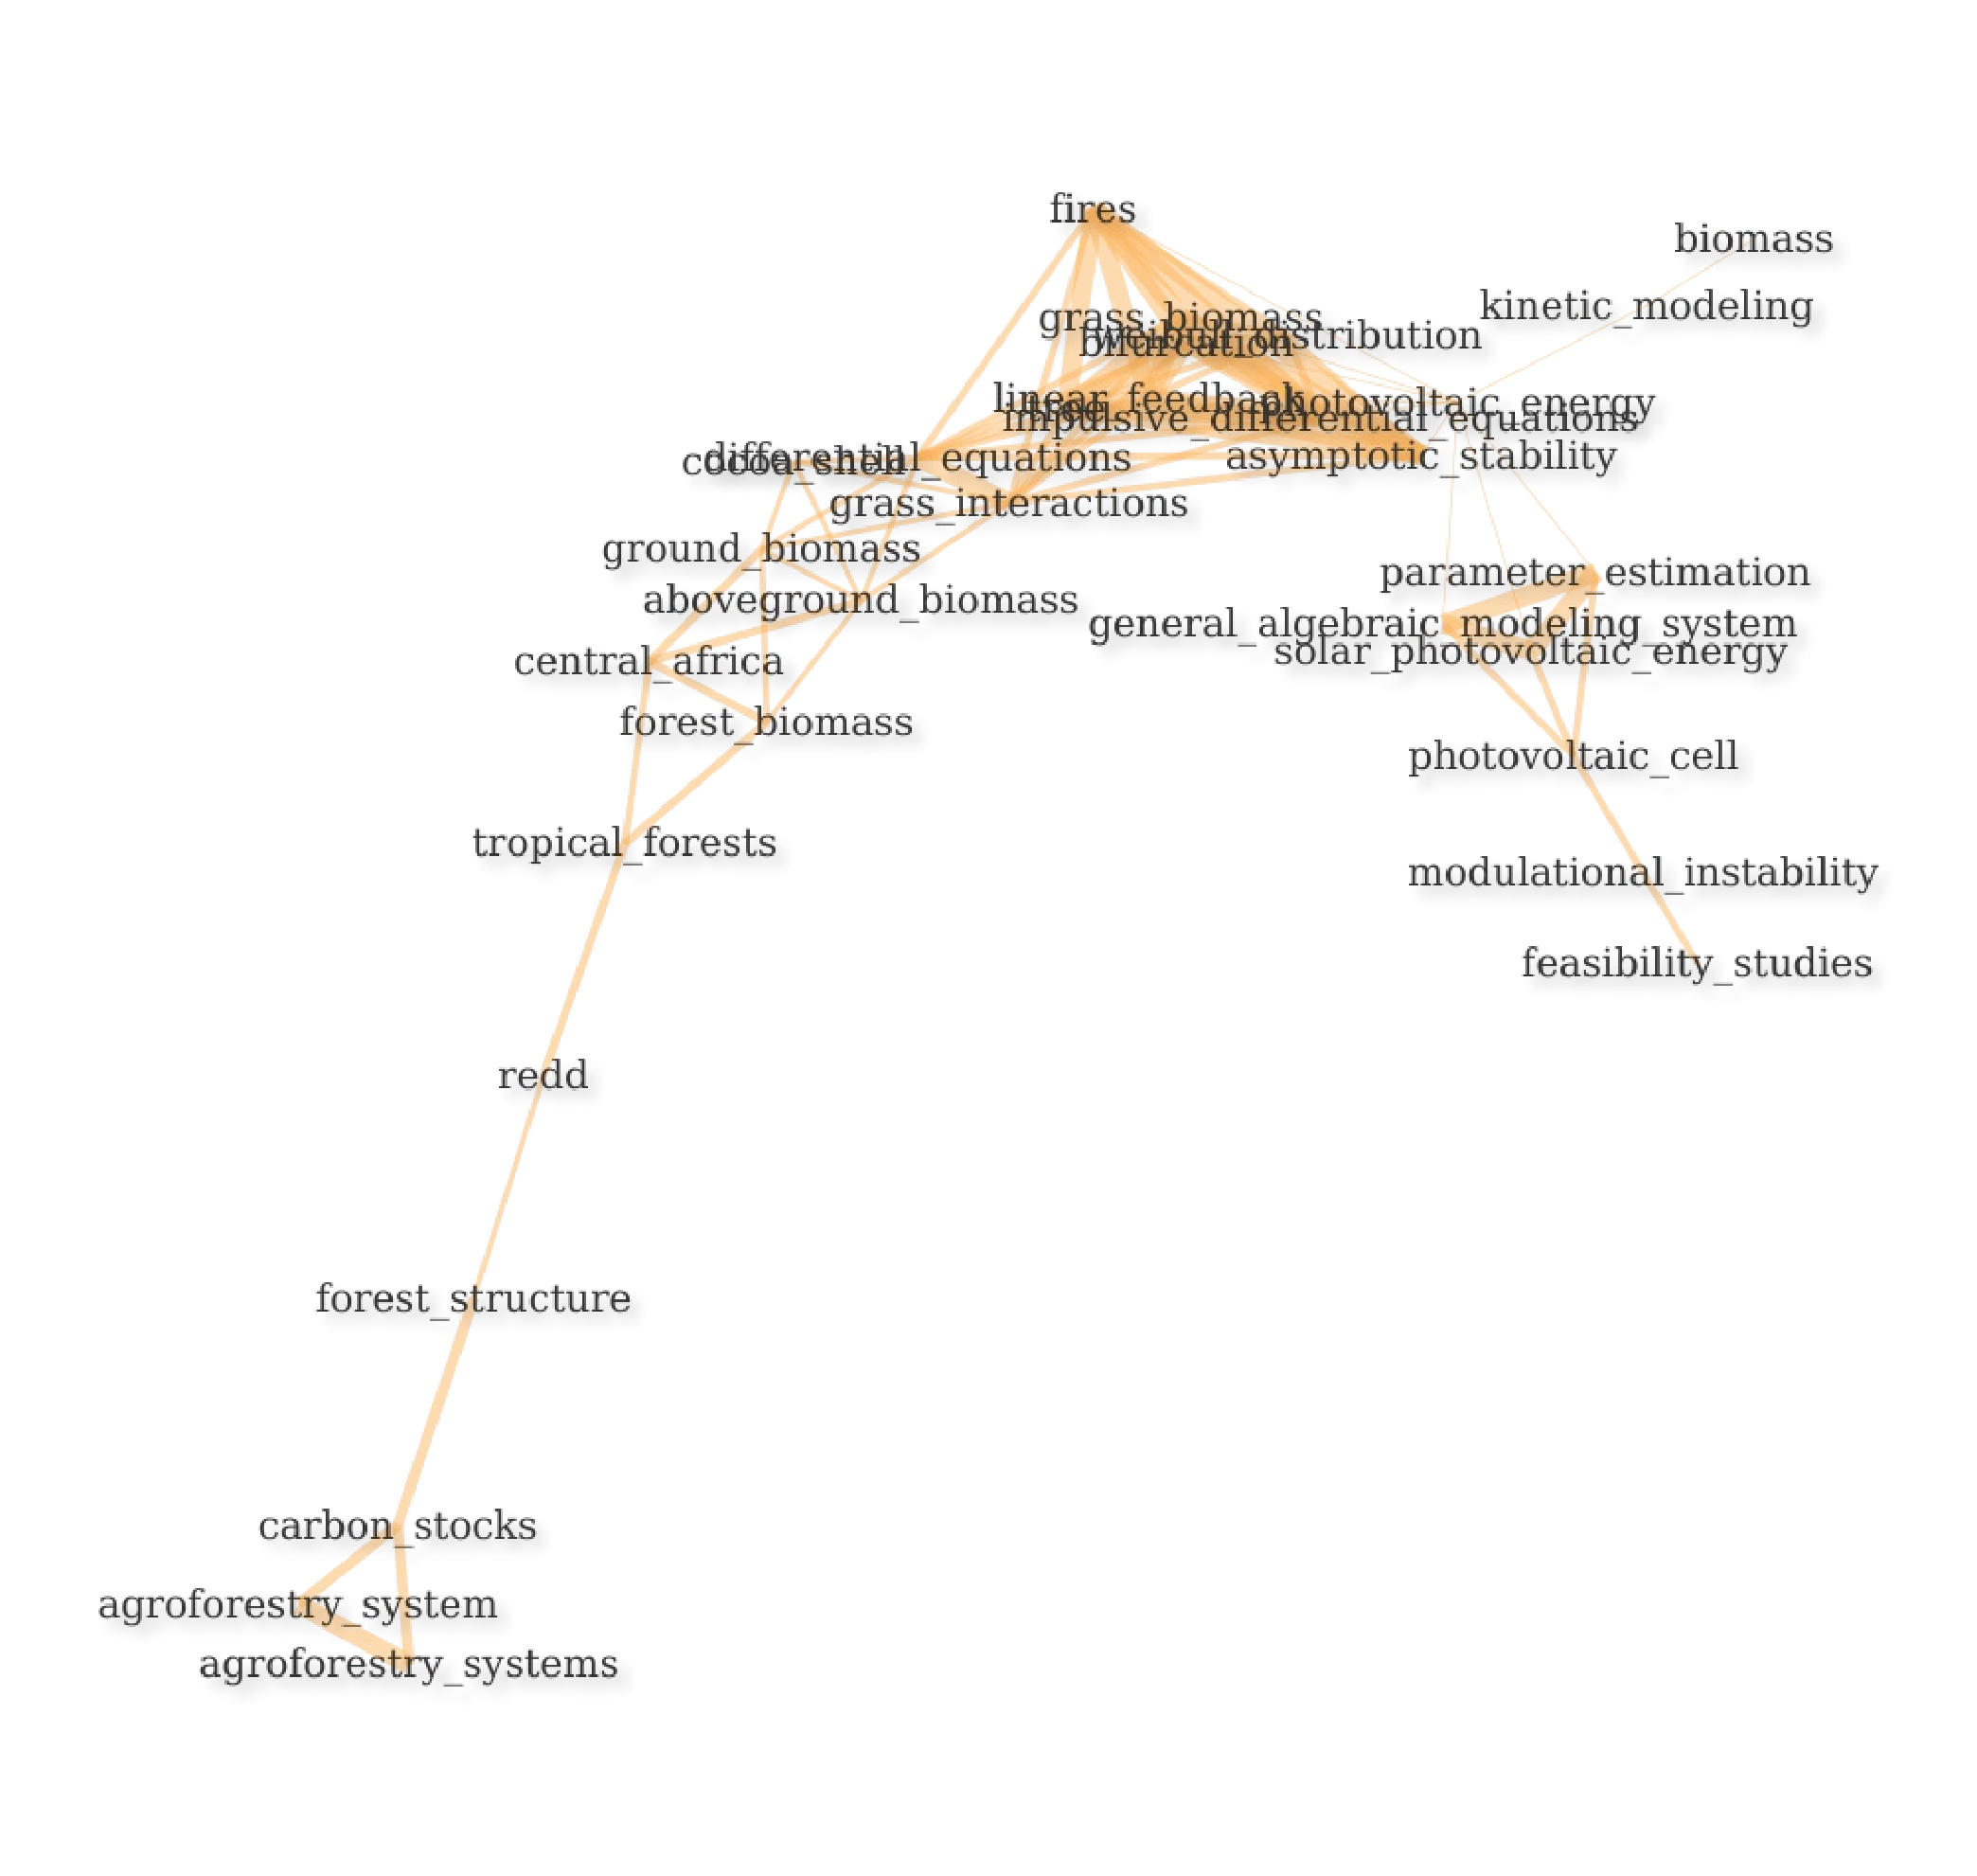
\includegraphics[width=1\linewidth]{01_bookdown_files/figure-latex/yaounngramnetwork-1} \caption{Keyword/keyword pair correlation network in RE-related publications of Université de Yaoundé I}\label{fig:yaounngramnetwork}
\end{figure}

Keyword/ keyword pair correlation network also shows the influence of the research area Forestry. Forest/ground biomass research along with tropical forest and forest structure topics shows the main directions of the Forestry research, we also see the use of cocoa shells for green energy often explored in the RE-related research of \emph{Université de Yaoundé I}.

Other than the biomass and solar energy-related topics keywords also indicates research on different modelling approaches.

\hypertarget{addis-ababa-university-ethiopia}{%
\paragraph{Addis Ababa University (Ethiopia)}\label{addis-ababa-university-ethiopia}}

\begin{figure}
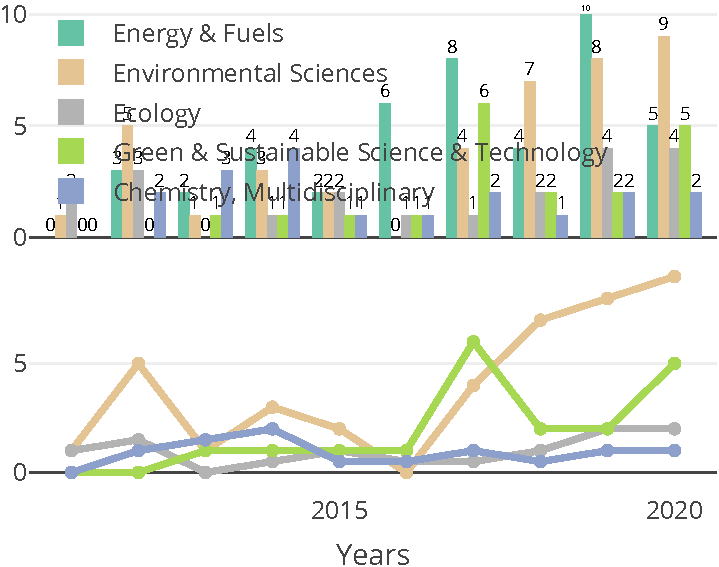
\includegraphics[width=1\linewidth]{01_bookdown_files/figure-latex/addisbarline-1} \caption{Absolute and relative growth of the most visible research areas in RE-related publications of Addis Ababa University between 2011-2020}\label{fig:addisbarline}
\end{figure}

Similar to the previous visible organisations the most visible research area in the RE-related research of \emph{Addis Ababa University} is Energy \& Fuels. However, Environmental Sciences is the most rapidly increasing area in the number of RE-related publications followed by Ecology, Green \& Sustainable Science \& Technology, and Multidisciplinary Chemistry.

\begin{figure}
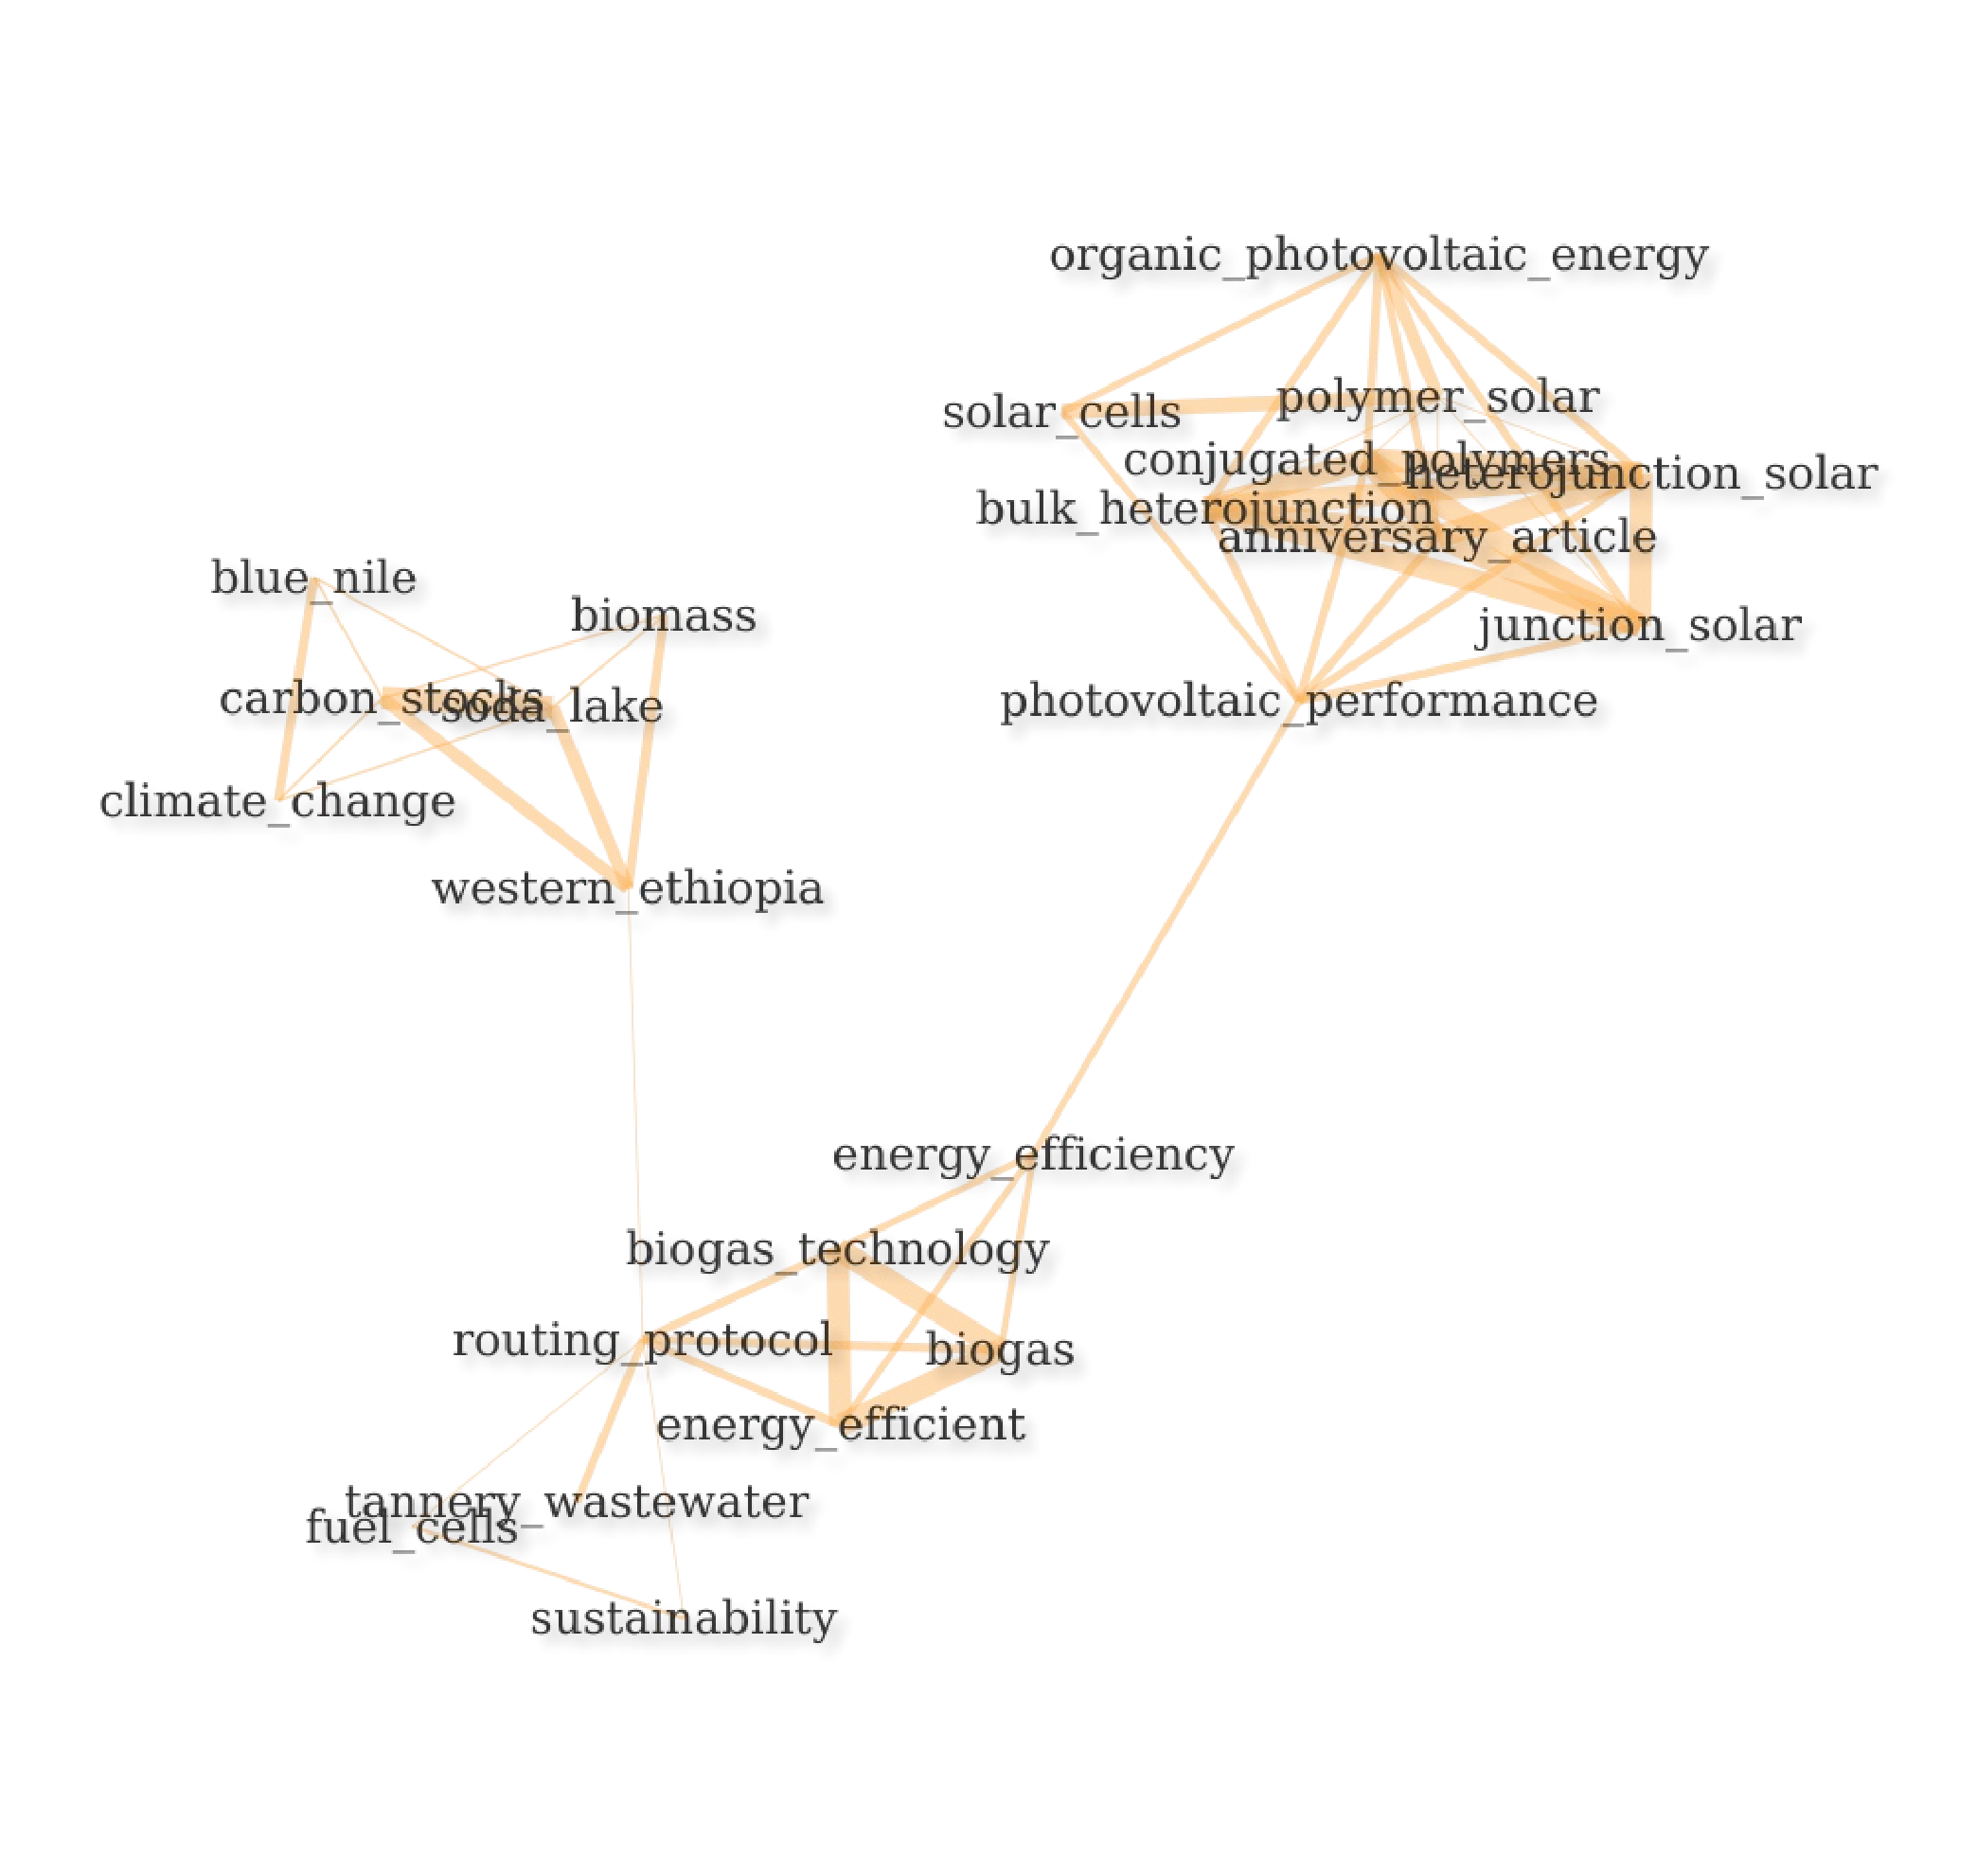
\includegraphics[width=1\linewidth]{01_bookdown_files/figure-latex/addisngramnetwork-1} \caption{Keyword/keyword pair correlation network in RE-related publications of Addis Ababa University}\label{fig:addisngramnetwork}
\end{figure}

3 clusters of the keyword/keyword pairs in the RE-related publications of \emph{Addis Ababa University} roughly include biomass, biogas, and solar energy related keywords. In the solar energy cluster, there are keyword pairs that indicate research on different production approaches for photovoltaic components like organic photovoltaic cells (OPV, see \protect\hyperlink{ref-rwenyagila2017}{Rwenyagila} (\protect\hyperlink{ref-rwenyagila2017}{2017})) and conversion technologies like the heterojunction approach.

In the biomass cluster, there is also the mention of soda lake as there are several soda lakes in the borders of Ethiopia, there is also the Blue Nile Project mentioned which is a massive hydroelectric project on Blue Nile River.

\hypertarget{mekelle-university-ethiopia}{%
\paragraph{Mekelle University (Ethiopia)}\label{mekelle-university-ethiopia}}

\begin{figure}
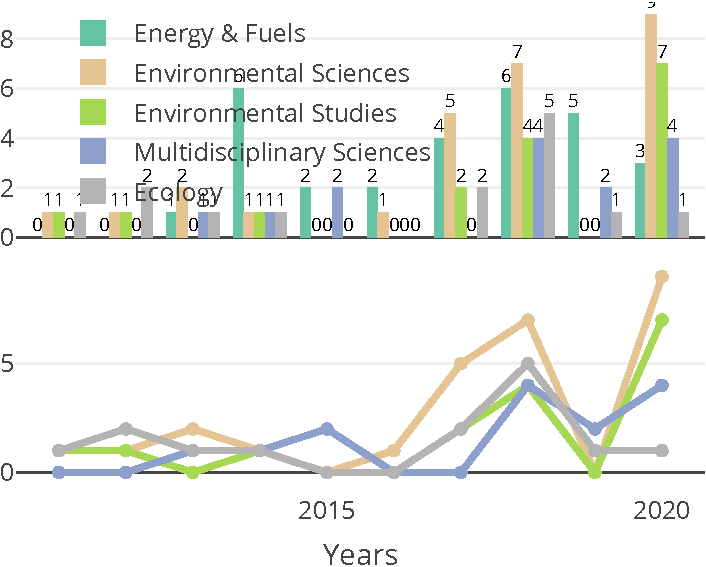
\includegraphics[width=1\linewidth]{01_bookdown_files/figure-latex/mekelbarline-1} \caption{Absolute and relative growth of the most visible research areas in RE-related publications of Mekelle University between 2011-2020}\label{fig:mekelbarline}
\end{figure}

The most visible research areas of \emph{Mekelle University} are Energy \& Fuels, Environmental Sciences, Environmental Studies, Multidisciplinary Sciences, and Ecology.
Both Environmental Studies and Sciences spike in 2020 after 0 RE-related publications in 2019.

\begin{figure}
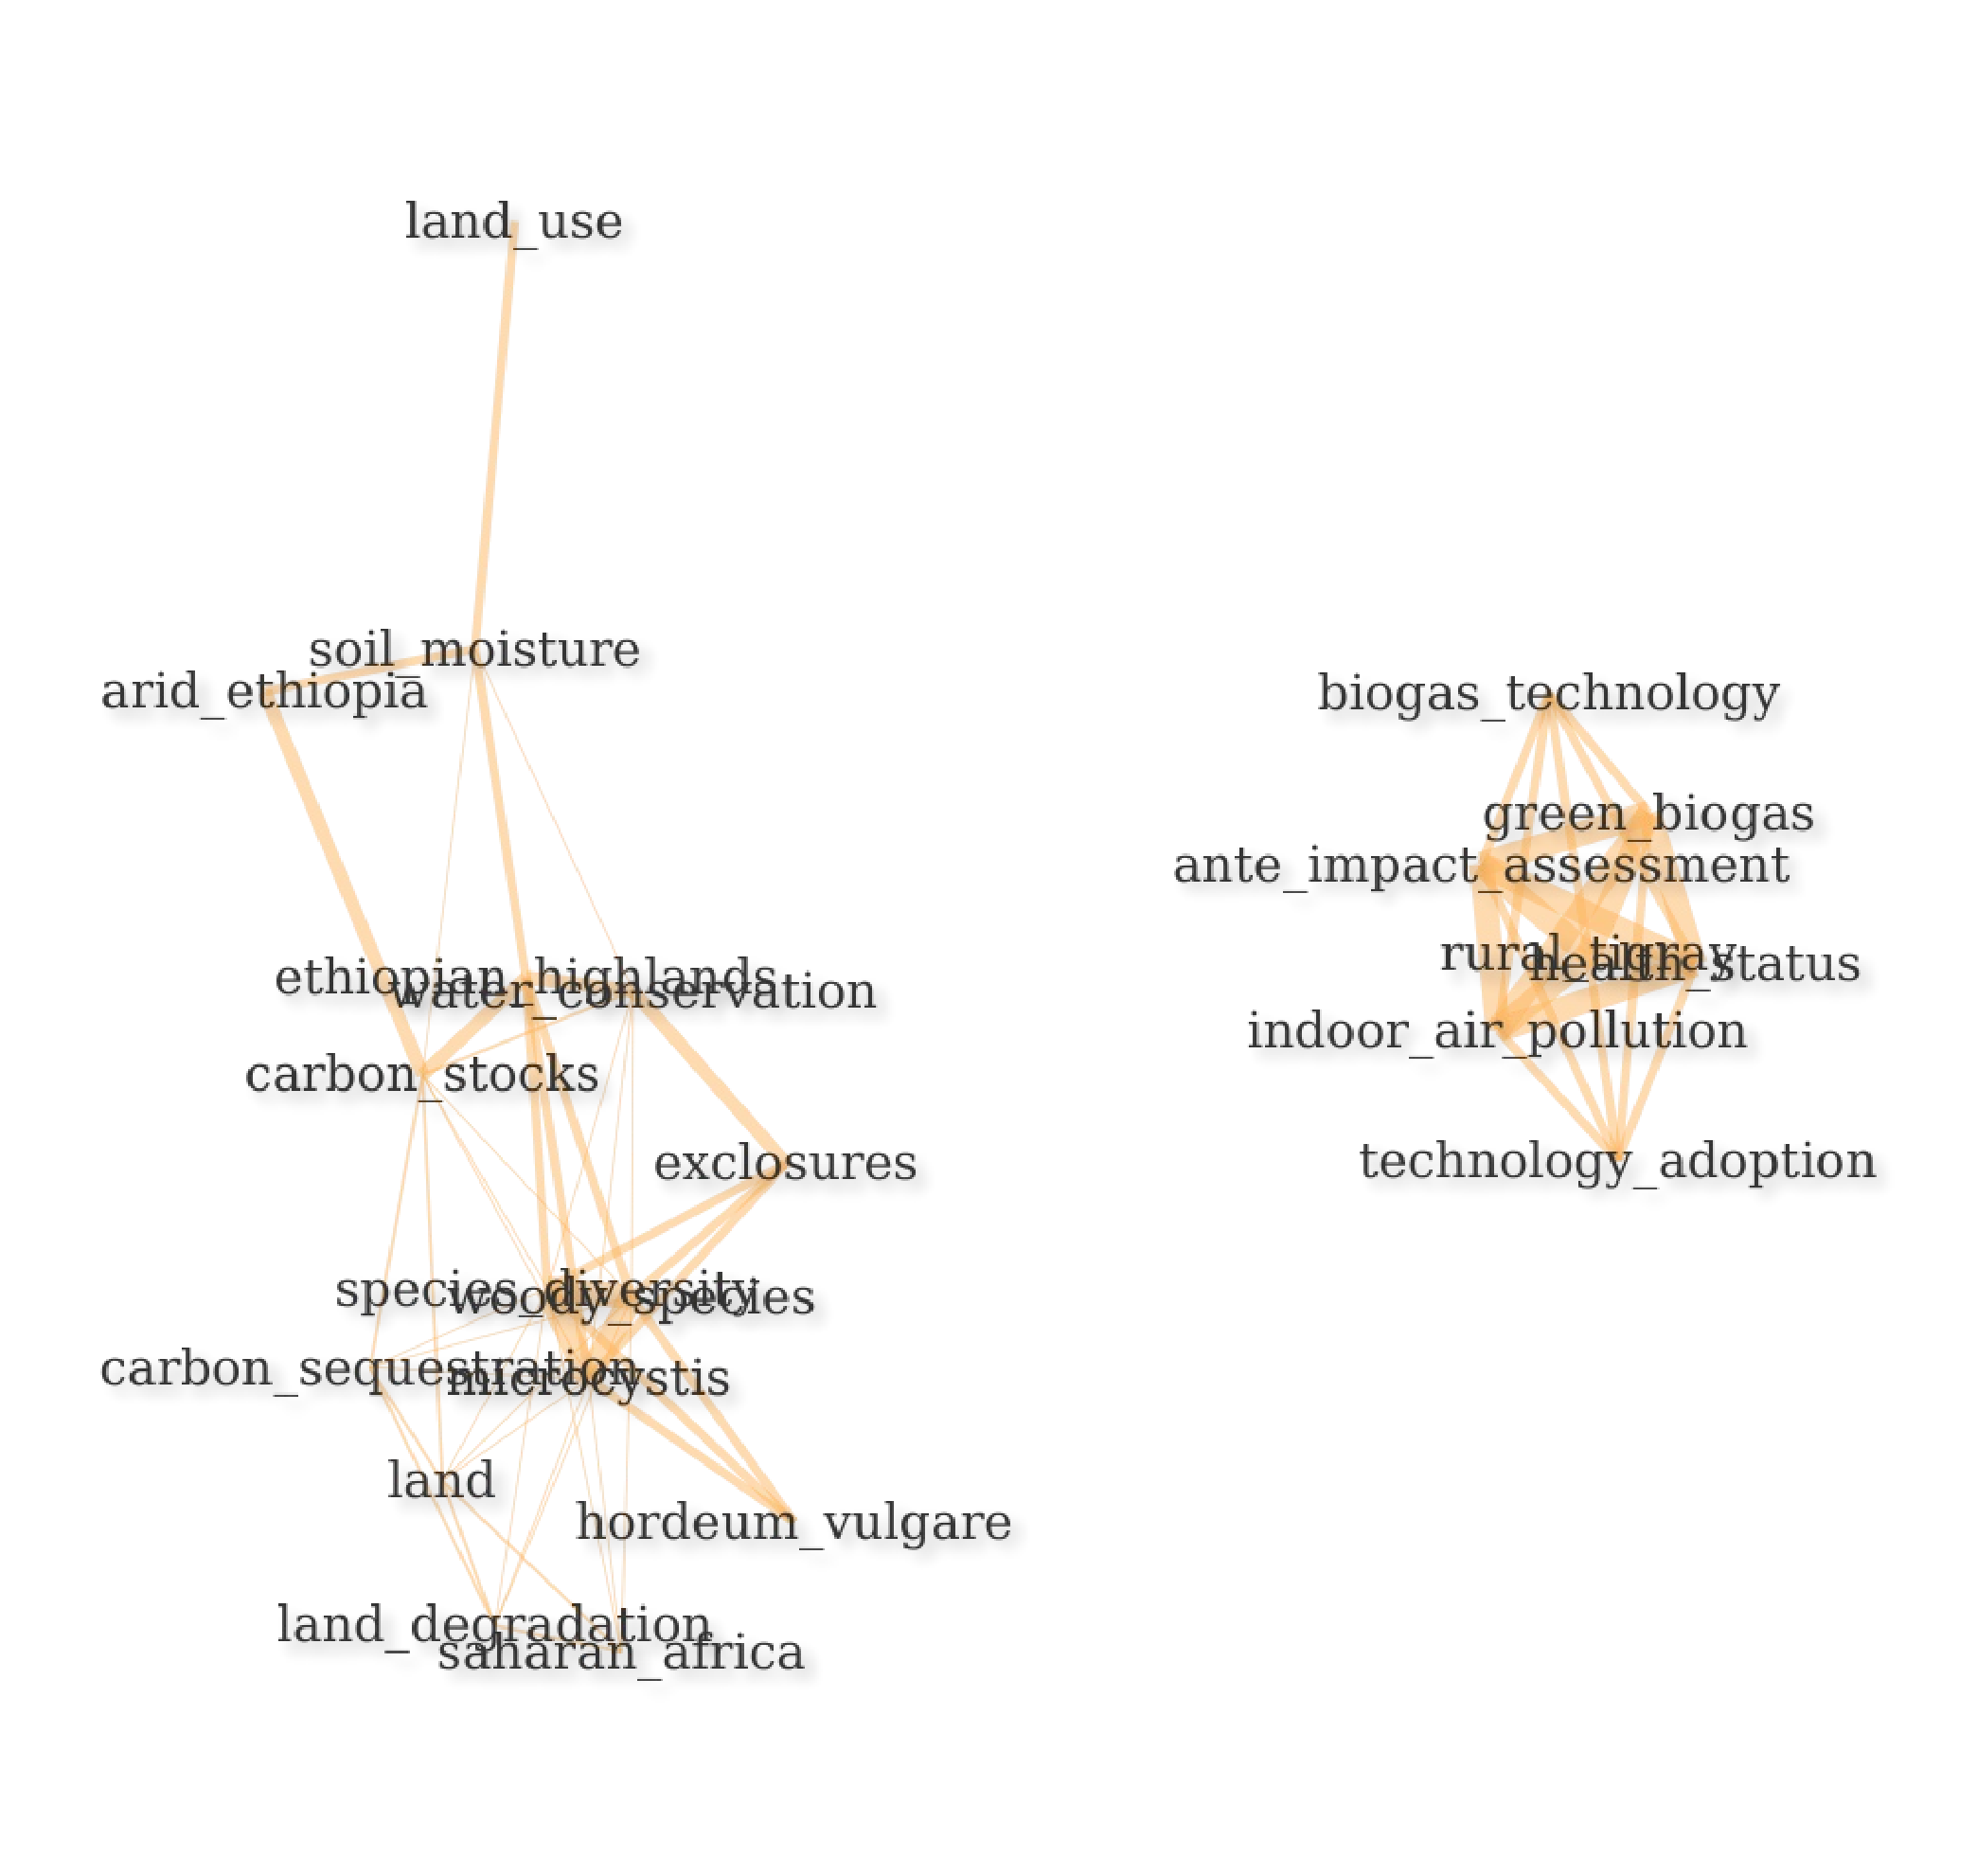
\includegraphics[width=1\linewidth]{01_bookdown_files/figure-latex/mekelngramnetwork-1} \caption{Keyword/keyword pair correlation network in RE-related publications of Mekelle University}\label{fig:mekelngramnetwork}
\end{figure}

\emph{Mekelle University}'s keyword pair correlation network displays 2 different clusters which can be roughly labelled as environmental topics and biogas related keywords.

In the first cluster, Ethiopia's environmental issues like land degradation, diversity of species, water conversation, soil moisture, better land use are the emphasized topics. In relation, there is a high number of publications that mention the use of by-product materials from trees and shrubs as biomass material.

In the second cluster along with the biogas topics, there is an emphasis on health status, indoor air pollution, remote communities like rural Tigray where is an ongoing crisis in the isolated because of the complete isolation from the outer world.

\hypertarget{southern-africa}{%
\subsection{Southern Africa}\label{southern-africa}}

\begin{figure}
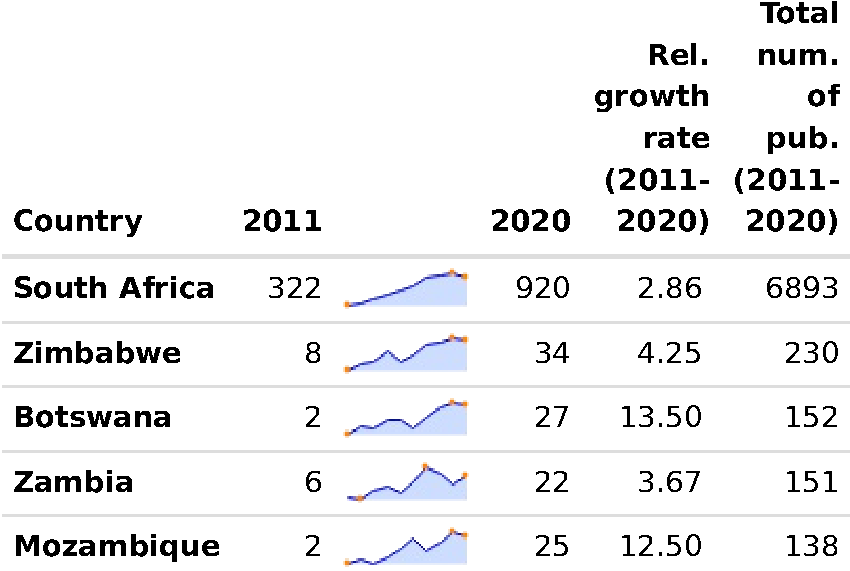
\includegraphics[width=1\linewidth]{01_bookdown_files/figure-latex/satable-1} \caption{RE-related publication output in Southern African countries}\label{fig:satable}
\end{figure}

There is a strong contrast between the Southern African countries in terms of RE-related publication output. While South Africa is the most visible country in the whole continent with \textasciitilde6900 RE-related publications between 2011-2020 the closest follower Zimbabwe have 230. Other than South Africa and Zimbabwe, the following countries Botswana, Zambia and Mozambique \textasciitilde150 RE-related publications between 2011-2020 each.

\begin{figure}

\includegraphics[width=1\linewidth]{01_bookdown_files/figure-latex/sanet-1} \caption{Co-publication network of Southern African countries in RE-related publications between 2011-2020}\label{fig:sanet}
\end{figure}

In alignment with the total number of publications, South Africa is the centre of mass in the co-publication network of Southern Africa. All the other visible South African countries have collaborations with South Africa with more than 25 co-publications. South Africa also has strong interregional collaboration with other African countries, which includes Egypt (\textasciitilde30 co-pub.) from Northern Africa; Nigeria (277 co-pub.) and Ghana (27 co-pub.) from Western Africa; Ethiopia (44 co-pub.), Tanzania (38 co-pub.), Uganda (32 co-pub.) and Kenya (68 co-pub.) from Eastern Africa, which makes South Africa the most visible African country also in interregional collaborations. None of the Southern African countries has a collaboration link with more than 25 co-pub. without the involvement of South Africa.

The most visible EU-27 country in the region is Germany with involvement in 373 co-publications. Germany is followed by France with 290 co-pub. and Spain 150 co-publications. However, South Africa's most visible collaborations are with the United Kingdom and the United States. Those collaborations constitute 533 out of UK's 614 and 701 out of US' 812 co-publications in the region.

\hypertarget{south-africa}{%
\subsubsection{South Africa}\label{south-africa}}

\textbackslash begin\{figure\}
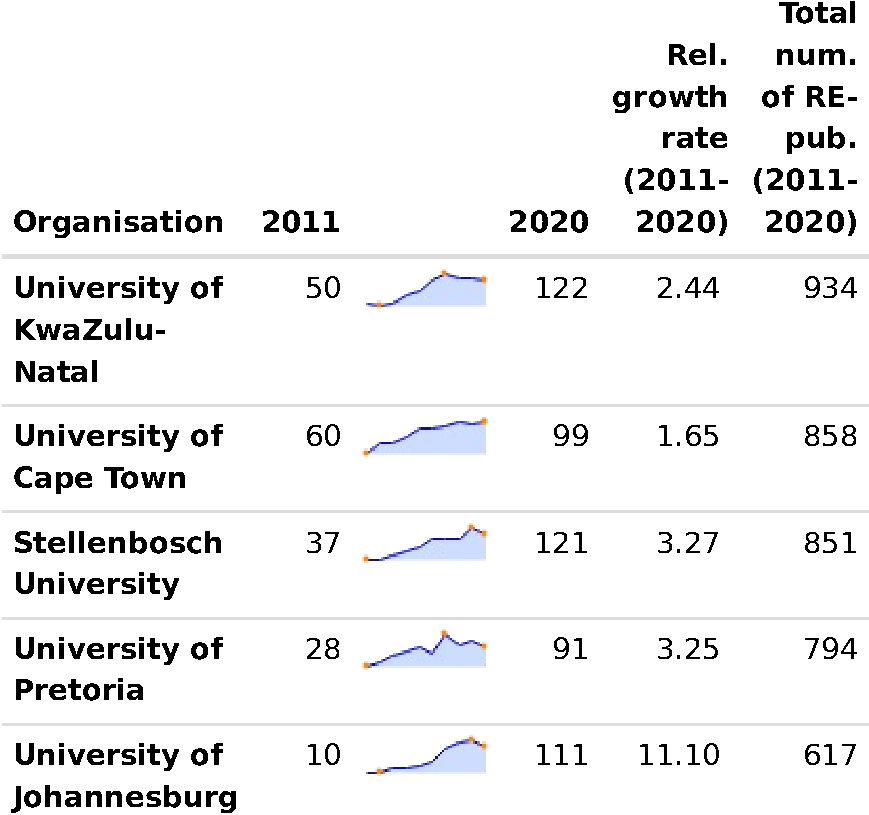
\includegraphics[width=0\linewidth]{01_bookdown_files/figure-latex/saorgtable-1}
The most visible 5 organisations in the region are all from South Africa. \emph{University of KwaZulu-Natal} is the organisation with the highest output of RE-related publications (934 publications). However, the organisation's RE-related publication output is stagnating since 2017.

\emph{University of Cape Town} is steadily increasing its RE-related publications since 2011 with a total output of \textasciitilde860 publications. \emph{Stellenbosch University} is closely following with \textasciitilde850 RE-related publications between 2011-2020 which despite the decline after 2019 only 1 publication behind \emph{University of KwaZulu-Natal}. \emph{University of Pretoria} and \emph{University of Johannesburg} are following with \textasciitilde800 and \textasciitilde620 publications respectively.

\begin{figure}
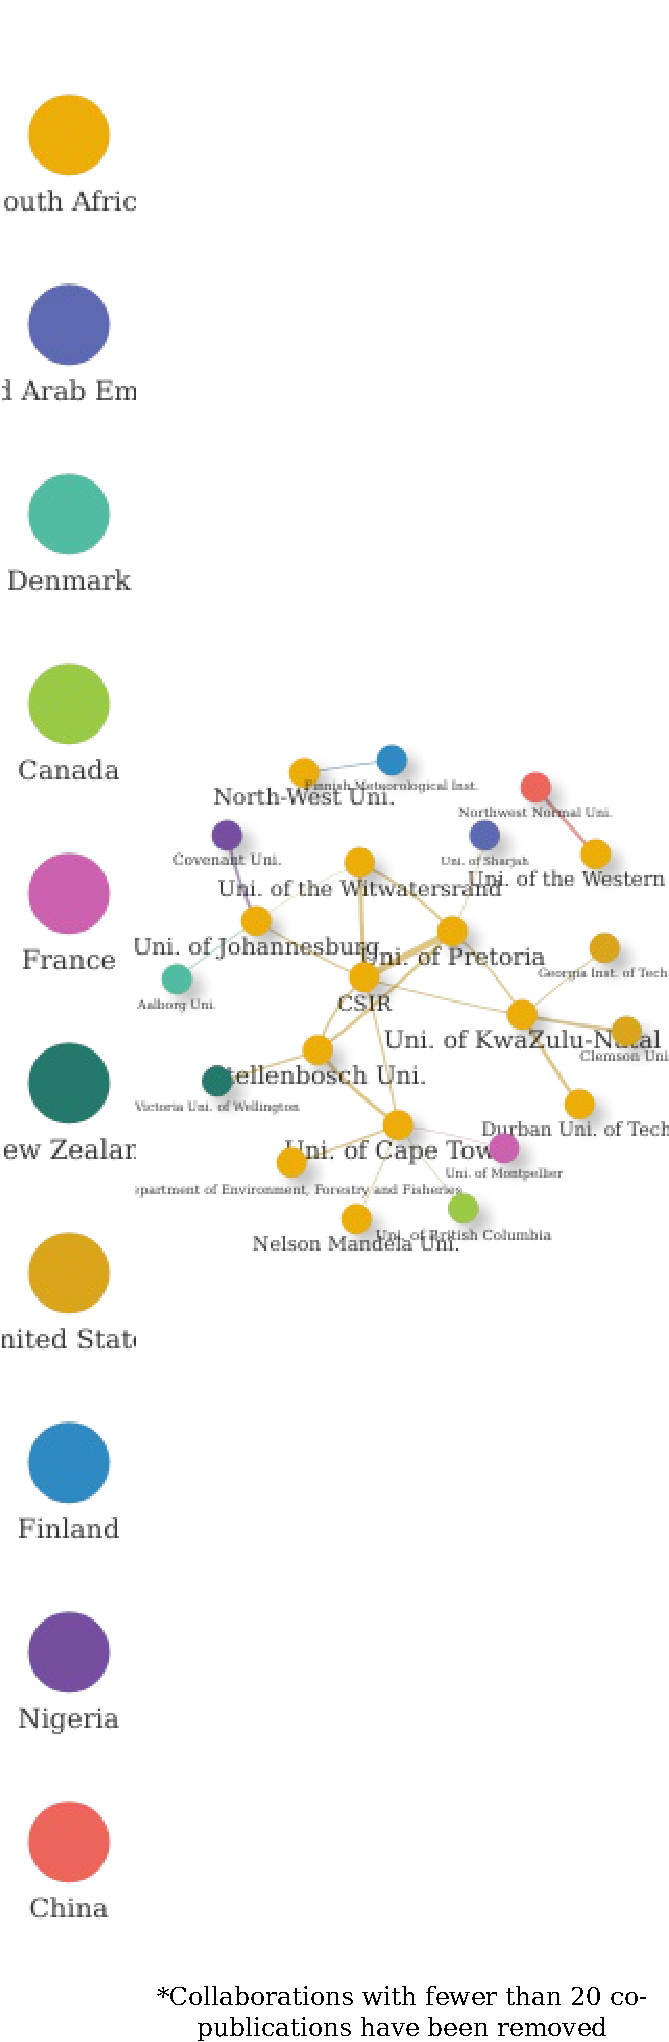
\includegraphics[width=1\linewidth]{01_bookdown_files/figure-latex/saorgnet-1} \caption{Co-publication network of Southern African organisations in RE-related publications between 2011-2020}\label{fig:saorgnet}
\end{figure}

The organisation network of South Africa displays a relatively well interconnected co-publication structure with a number of intercontinental collaborators. None of the organisations seems to be the centre of mass in the network.

Some of the notable international collaborations are between China's \emph{Northwest Normal University} and \emph{University of Western Cape} (36 co-pub.), Denmark's \emph{Aalborg University} and \emph{University of Johannesburg} (23 co-pub,), UAE's \emph{Uni. of Sharjah} and \emph{University of Pretoria} (22 co-pub.), New Zealand's \emph{Victoria University of Wellington} and \emph{Stellenbosch University} (\textasciitilde30 co-pub.), France's \emph{University of Montpellier} and \emph{University of Cape Town} (20 co-pub.) and Canada's \emph{Uni. of British Columbia} and \emph{University of Cape Town} (23 co-pub.). Also, as an interregional collaboration between African organisations, Nigeria's \emph{Covenant University} has 34 RE-related co-publications with \emph{University of Johannesburg}.

\hypertarget{university-of-kwazulu-natal}{%
\paragraph{University of KwaZulu-Natal}\label{university-of-kwazulu-natal}}

\begin{figure}
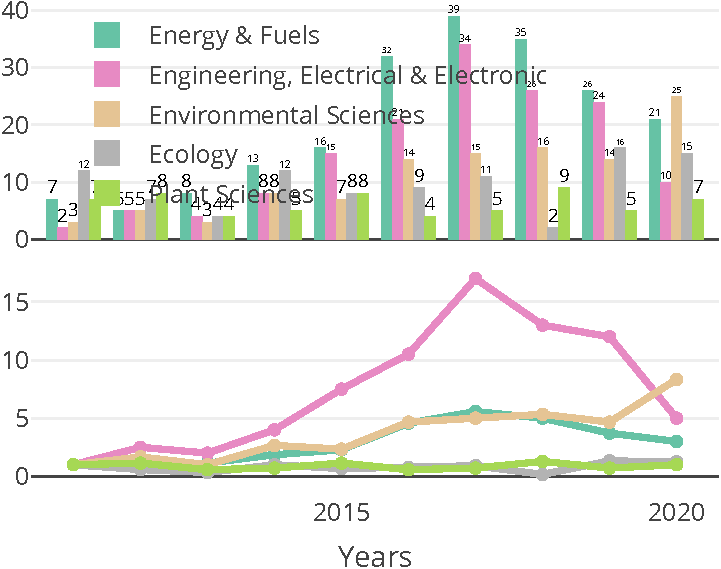
\includegraphics[width=1\linewidth]{01_bookdown_files/figure-latex/kwazubarline-1} \caption{Absolute and relative growth of the most visible research areas in RE-related publications of University of KwaZulu-Natal between 2011-2020}\label{fig:kwazubarline}
\end{figure}

The most visible areas in \emph{University of KwaZulu-Natal}'s publications are Energy \& Fuels and Electrical \& Electronic Engineering. However, as seen previously in other organisations both of those fields start to decline in numbers after 2017. Instead, the number of publications in Environmental Sciences keeps growing followed by Ecology in a relatively stable manner. Other than this reoccurring pattern \emph{University of KwaZulu-Natal} has uniquely Plant Sciences as one of the most visible areas.

\begin{figure}
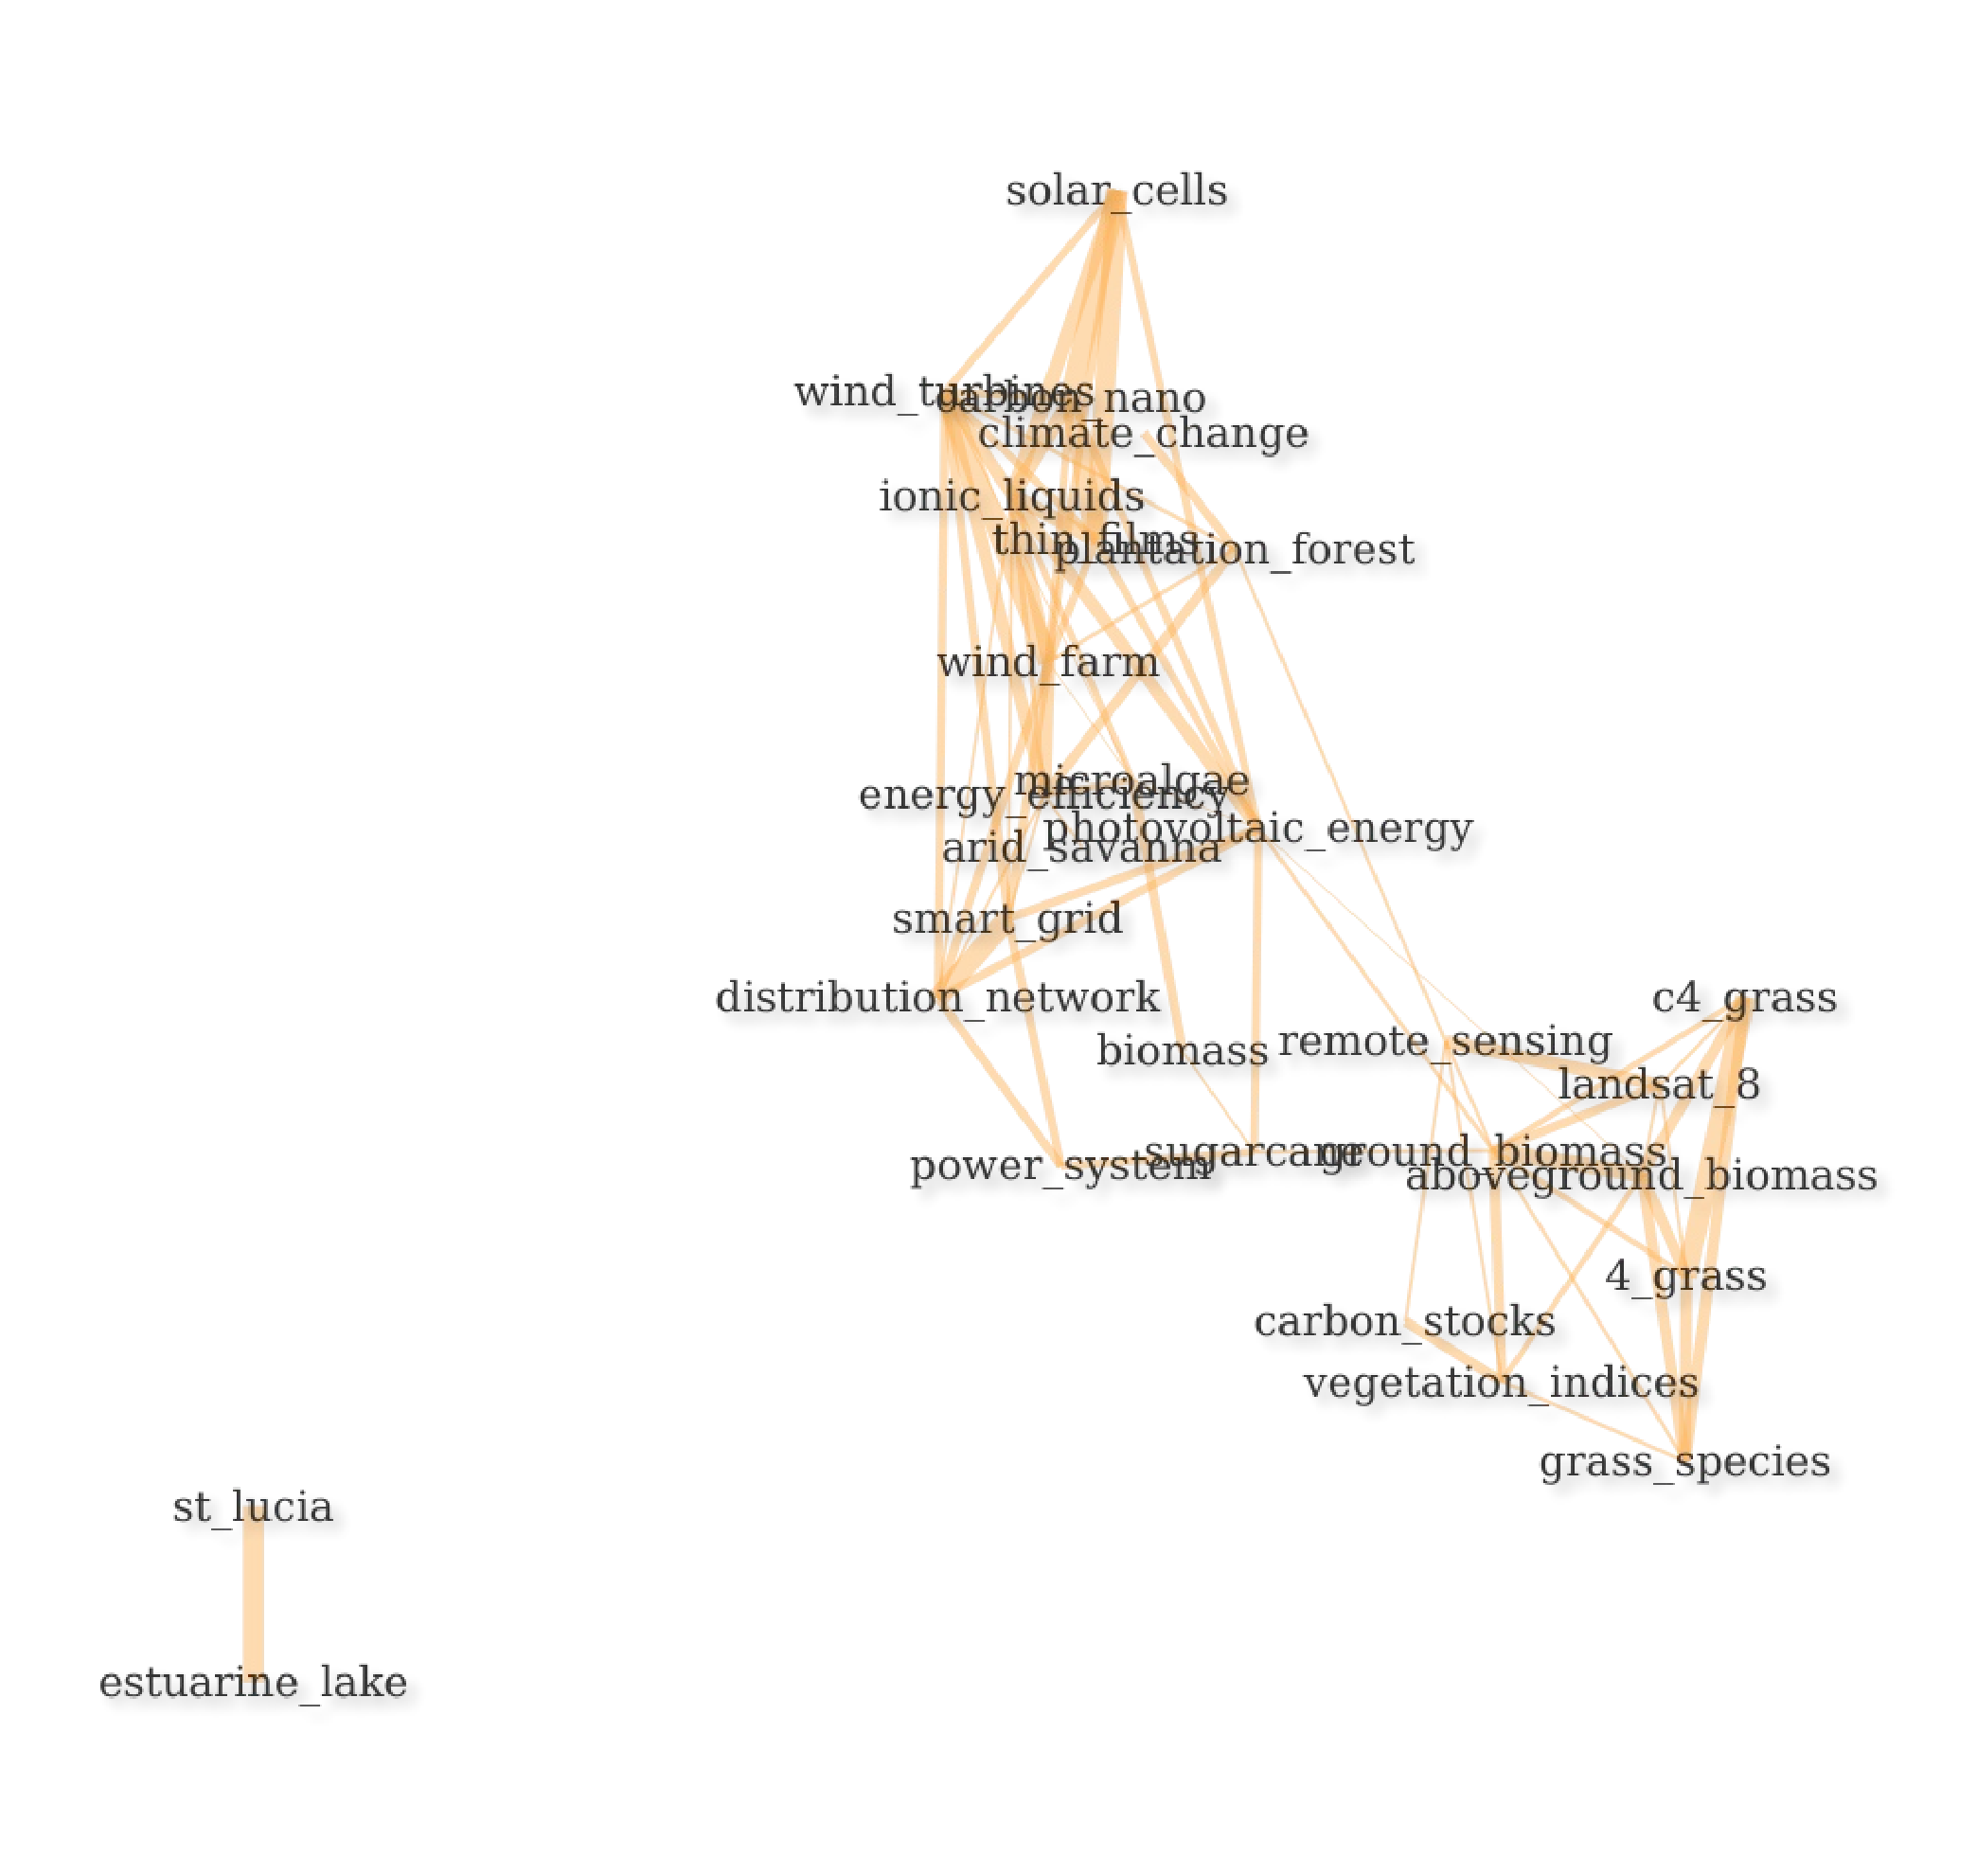
\includegraphics[width=1\linewidth]{01_bookdown_files/figure-latex/kwazungramnetwork-1} \caption{Keyword/keyword pair correlation network in RE-related publications of University of KwaZulu-Natal}\label{fig:kwazungramnetwork}
\end{figure}

As unique keyword pairs, \emph{University of KwaZulu-Natal}'s keyword correlation network includes the mention of estuarine lakes. The exploitation of the tidal energy where salty and freshwater meet is an often discussed topic (see for example \protect\hyperlink{ref-ross2021}{Ross et al.} (\protect\hyperlink{ref-ross2021}{2021})) and the largest estuarine lake in Southern Africa, namely Saint Lucia, is located in South Africa.

Other keyword pairs show great diversity. Generally trending topics like solar and wind energy-related keyword pairs are also present in \emph{University of KwaZulu-Natal}'s network. As a unique biomass related keyword, c4 grass type is often mentioned in the publications in \emph{University of KwaZulu-Natal} which ar referring to a specific type of grass that can be used effectively for biofuel production (see \protect\hyperlink{ref-vanderweijde2013}{van der Weijde et al.} (\protect\hyperlink{ref-vanderweijde2013}{2013})).

\hypertarget{university-of-cape-town}{%
\paragraph{University of Cape Town}\label{university-of-cape-town}}

\begin{figure}
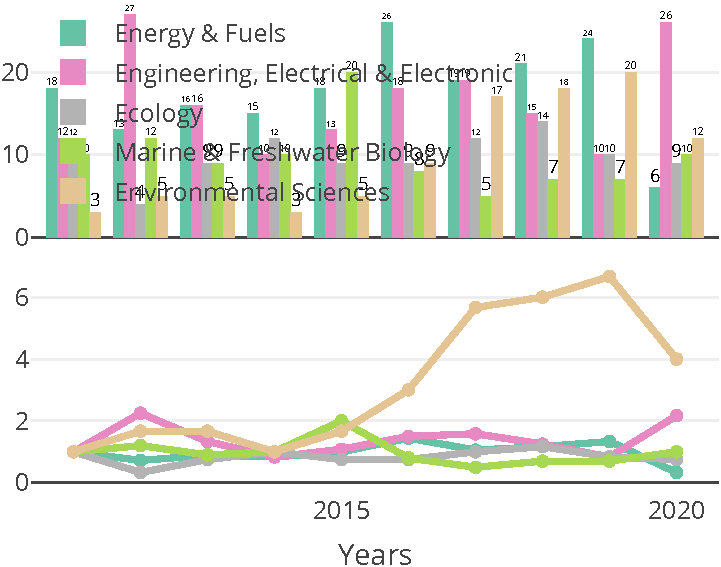
\includegraphics[width=1\linewidth,height=700px]{01_bookdown_files/figure-latex/capetbarline-1} \caption{Absolute and relative growth of the most visible research areas in RE-related publications of University of Cape Town between 2011-2020}\label{fig:capetbarline}
\end{figure}

Similar to \emph{University of KwaZulu-Natal}, the most visible research areas in the RE-related publications of \emph{University of Cape Town} are Energy \& Fuels and Electrical \& Electronic Engineering followed by Ecology. Uniquely, the most visible 5 research areas of \emph{University of Cape Town} include Marine \& Freshwater Biology which stays number of publication wise relatively stable over the years. Despite the decline in numbers in 2020 Environmental Sciences is steadily growing in numbers.

\begin{figure}
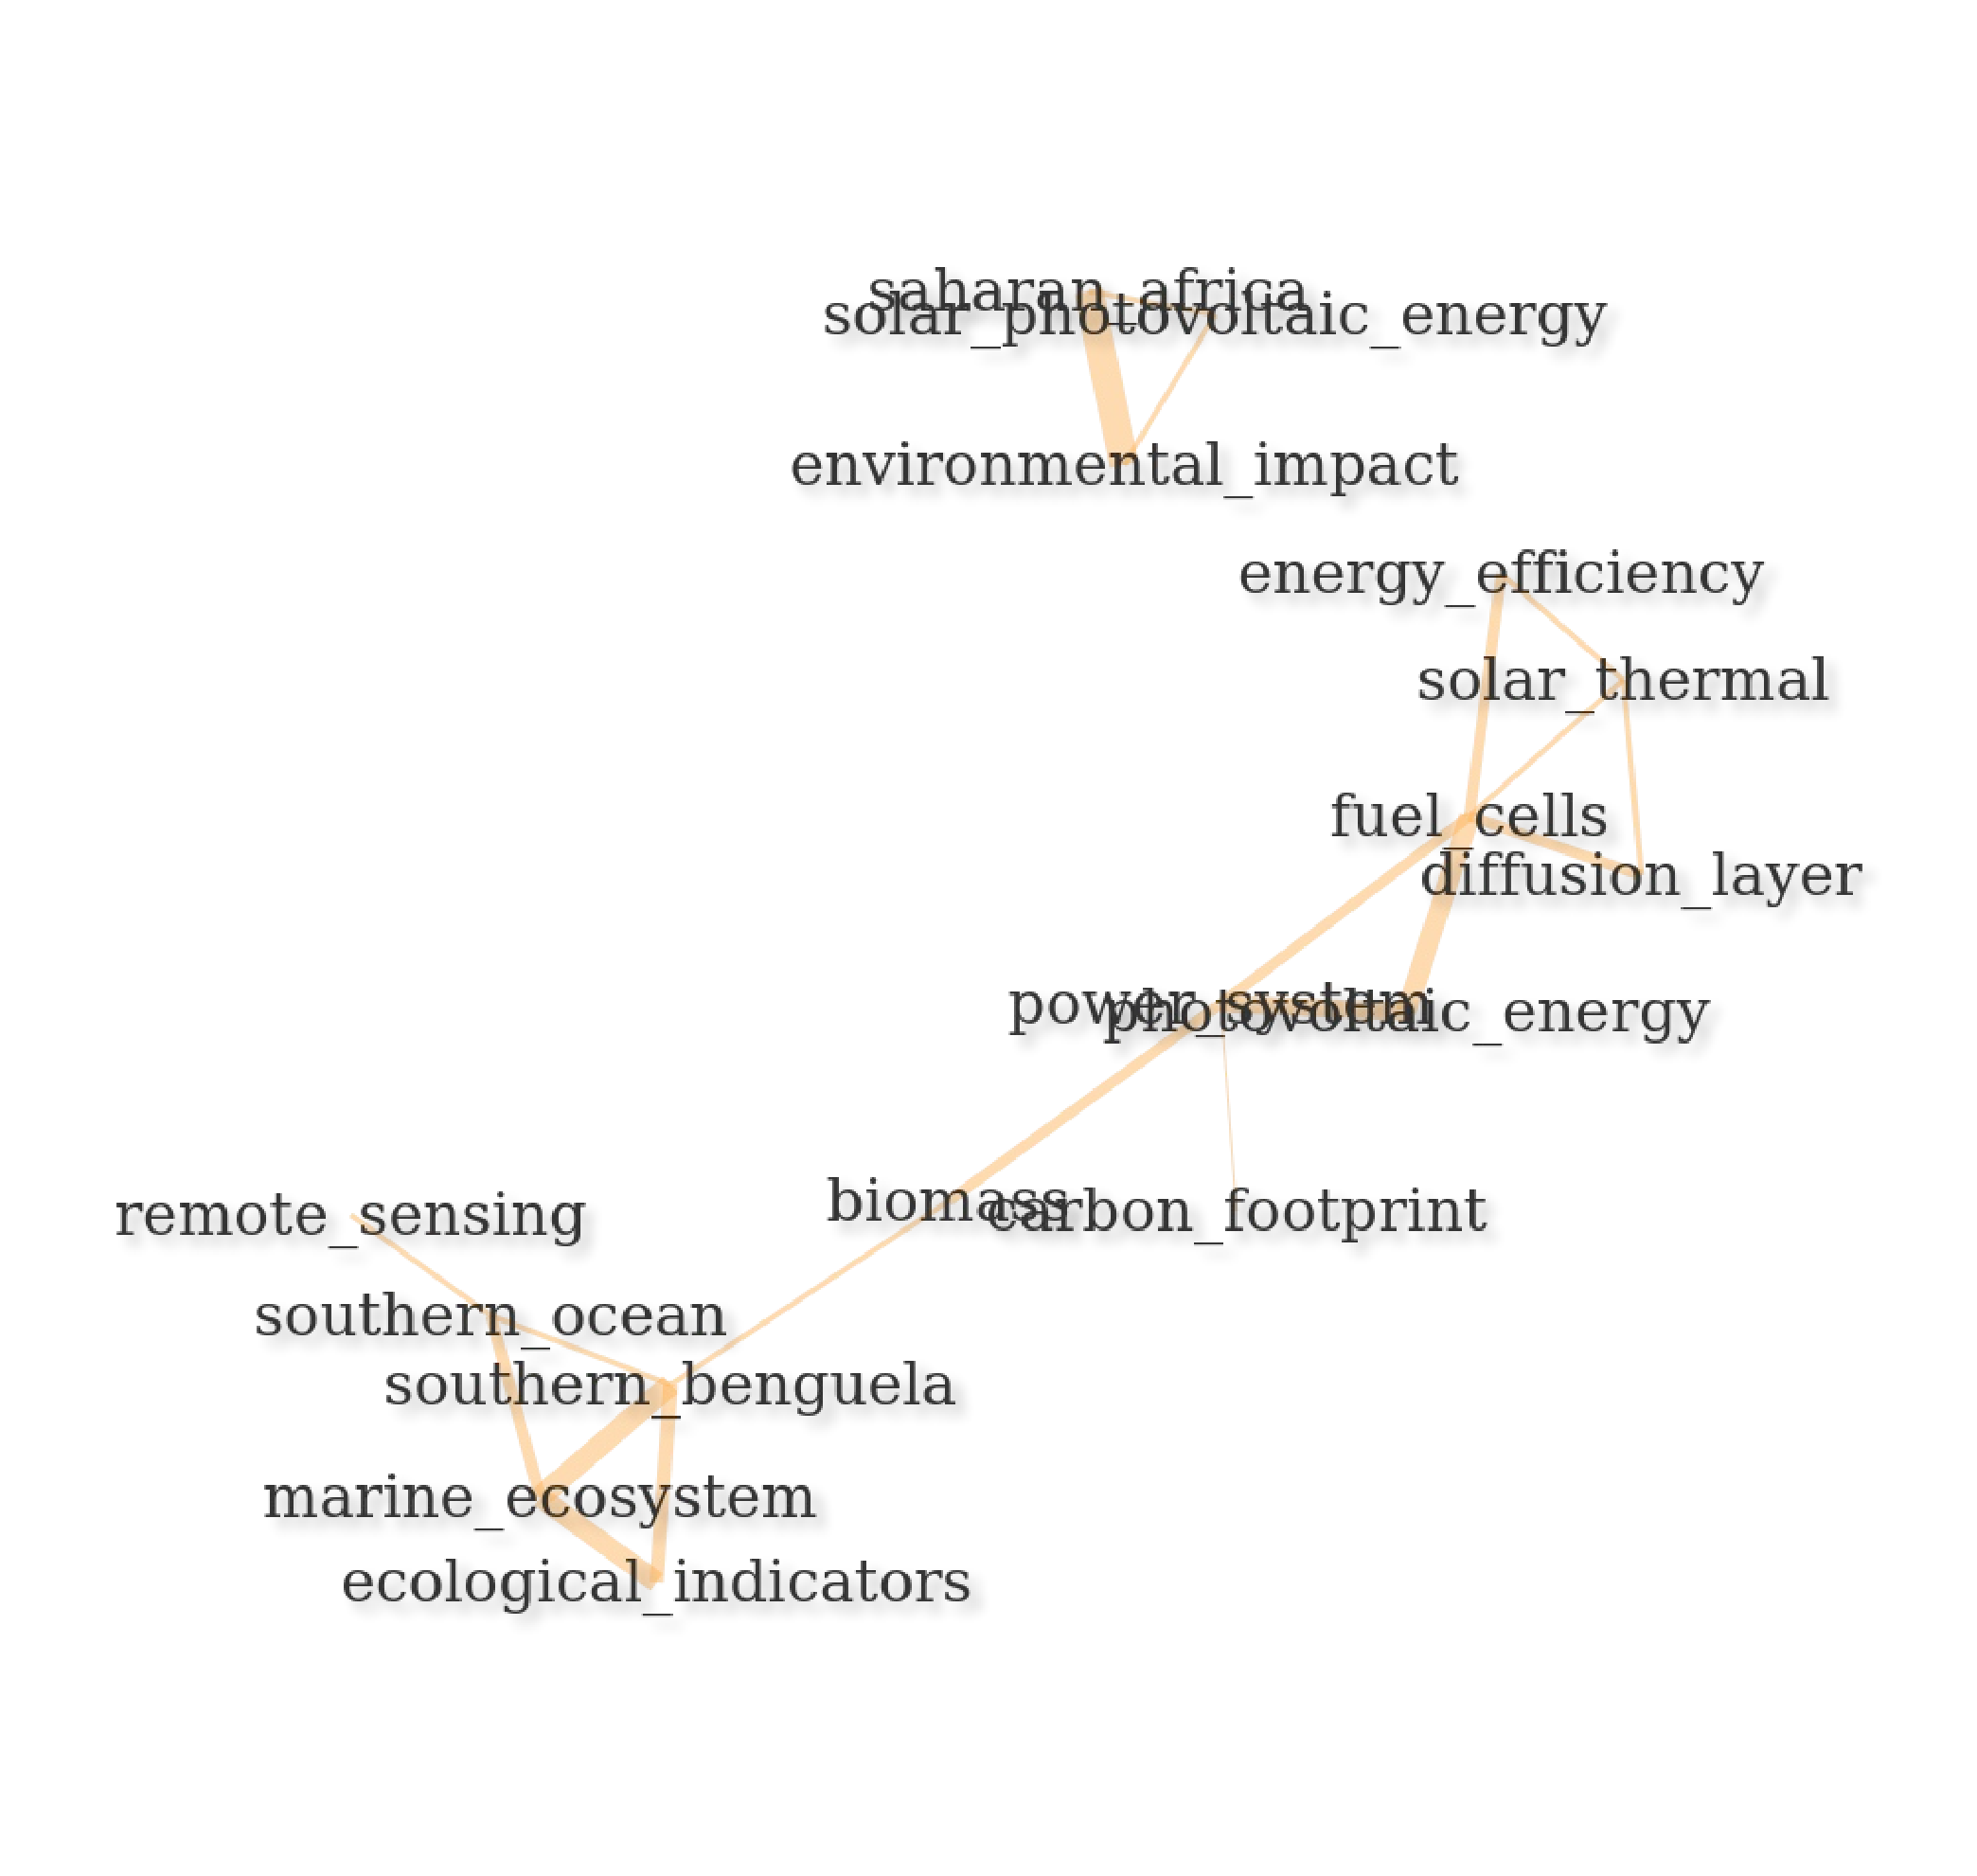
\includegraphics[width=1\linewidth]{01_bookdown_files/figure-latex/capetngramnetwork-1} \caption{Keyword/keyword pair correlation network in RE-related publications of University of Cape Town}\label{fig:capetngramnetwork}
\end{figure}

\emph{University of Cape Town}'s keyword/keyword pair network clearly shows the influence of Marine \& Freshwater Biology in one of its clusters. Marine ecosystem especially in Southern Benguela is a reoccurring topic in the publications of the \emph{University of Cape Town}.

Other than that, along with the high emphasis on photovoltaic energy environmental topics like environmental impact and carbon footprint are also visible keyword pairs.

\hypertarget{stellenbosch-university}{%
\paragraph{Stellenbosch University}\label{stellenbosch-university}}

\begin{figure}
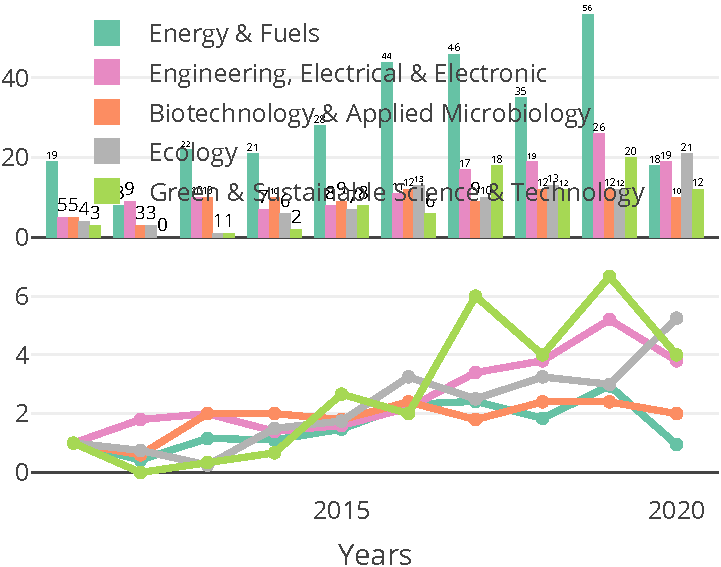
\includegraphics[width=1\linewidth]{01_bookdown_files/figure-latex/stellbarline-1} \caption{Absolute and relative growth of the most visible research areas in RE-related publications of Stellenbosch University between 2011-2020}\label{fig:stellbarline}
\end{figure}

Similar to the other South African organisations \emph{Stellenbosch University}'s most visible research areas are Energy \& Fuels and Electrical \& Electronic Engineering. A unique research area Biotechnology \& Applied Microbiology is following the most visible 2 research areas in a consistent manner. Ecology and Green \& Sustainable Science \& Technology are following those with Ecology having the highest number of publications in 2020.

\begin{figure}
\includegraphics[width=1\linewidth]{01_bookdown_files/figure-latex/stellngramnetwork-1} \caption{Keyword/keyword pair correlation network in RE-related publications of Stellenbosch University }\label{fig:stellngramnetwork}
\end{figure}

Wind energy-related keyword pairs are emphasised more in the publications of \emph{Stellenbosch University} than in any other South African country.

Research on types of yeast like Pichia Pastoris and fungi like Saccharomyces Cerevisiae presumably because of the high number of publications in Biotechnology \& Applied Microbiology (see \protect\hyperlink{ref-benjamin2020}{Benjamin, Bakare, and Effiong} (\protect\hyperlink{ref-benjamin2020}{2020}) and \protect\hyperlink{ref-siripong2018}{Siripong et al.} (\protect\hyperlink{ref-siripong2018}{2018}) for their possible uses for RE).

Other than that, a number of biomass, biogas and bioprocessing methods are also highly emphasised in the RE-related publications of \emph{Stellenbosch University}.

\hypertarget{domain-analysis}{%
\section{Domain Analysis}\label{domain-analysis}}

This chapter is mainly interested in analysing RE-related publications of African countries separated into the 5 research domains (Physical Sciences, Technology, Life Sciences \& Biomedicine, Social Sciences, and Arts \& Humanities) in order to offer a different perspective on the characteristics by reviewing the most visible institutional pairings and trending themes in each category. In order to exclude pairings from the same country institutional pairings have been chosen from the collaborations with at least an interregional partnership.

\hypertarget{physical-sciences}{%
\subsection{Physical Sciences}\label{physical-sciences}}

Country 1

Partner 1

Num. of co-pub.

Partner 2

Country 2

Most Visible Res. Area

Northern Africa

{Egypt }

{Minia University }

{45}

{JeonBuk National University }

{South Korea }

{Chemistry, Physical }

{Egypt }

{Minia University }

{32}

{King Saud University }

{Saudi Arabia }

{Chemistry, Physical }

{Egypt }

{Ain Shams University }

{22}

{King Khalid University }

{Saudi Arabia }

{Materials Science, Multidisciplinary}

{Egypt }

{Mansoura University }

{22}

{Ruhr University Bochum }

{Germany }

{Astronomy \& Astrophysics }

{Egypt }

{Tanta University }

{21}

{Jiangsu University }

{China }

{Chemistry, Analytical }

Western, Central, Eastern Africa

{Nigeria }

{Covenant University }

{17}

{University of Johannesburg }

{South Africa }

{Materials Science, Multidisciplinary}

{Cameroon }

{Université de Yaoundé I }

{13}

{University of Montpellier }

{France }

{Multidisciplinary Sciences }

{Cameroon }

{Université de Yaoundé I }

{11}

{University of Leeds }

{United Kingdom}

{Multidisciplinary Sciences }

{Gabon }

{National Agency for National Parks}

{10}

{University of Stirling }

{United Kingdom}

{Multidisciplinary Sciences }

{Gabon }

{National Agency for National Parks}

{10}

{University of Leeds }

{United Kingdom}

{Multidisciplinary Sciences }

Southern Africa

{South Africa}

{University of the Western Cape }

{36}

{Northwest Normal University }

{China }

{Electrochemistry }

{South Africa}

{North-West University }

{23}

{Finnish Meteorological Institute}

{Finland }

{Meteorology \& Atmospheric Sciences }

{South Africa}

{North-West University }

{18}

{University of Stuttgart }

{Germany }

{Polymer Science }

{South Africa}

{University of the Witwatersrand }

{13}

{Delft University of Technology }

{Netherlands }

{Chemistry, Multidisciplinary }

{South Africa}

{North-West University }

{12}

{Ruhr University Bochum }

{Germany }

{Astronomy \& Astrophysics }

Looking at the international collaborations in the research domain of Physical Sciences the top pairings seems to be the co-publication partnerships between African and East Asian countries. Co-publication partnership between Egypt's \emph{Minia University} and South Korea's \emph{JeonBuk National University} is the most visible one in terms of RE-related number of co-publications followed by the collaboration between \emph{University of the Western Cape} of South Africa and China's \emph{Northwest Normal University}.

The most visible Co-publication pairings in Northern and South Africa are occupied by Egyptian and South African organisations because of their high number of RE-related publication outputs. Egypt's high number of co-publications with Saudi Arabian institutions is also visible among the pairings, 2 of the most visible 5 pairings are between Egypt's \emph{Minia} and \emph{Ain Shams Universities} collaboration with Saudi Arabia's \emph{King Saud} and \emph{King Khalid Universities} respectively. 2. and 3. of the 5 most visible pairings in Southern Africa belong to \emph{North-West University} of South Africa with \emph{Finnish Meteorological Institute} and \emph{University of Stuttgart}.

In the Western, Central and Eastern Africa cluster the most visible pairing is between Nigeria's \emph{Covenant University} with South African \emph{University of Johannesburg} which is the only interregional African collaboration in the most visible co-publication collaborations in Physical Sciences. Other than \emph{Université de Yaoundé I}'s (Cameroon) collaborations with \emph{University of Montpellier} of France and the UK's \emph{University of Leeds} are also in the most visible organisational pairings. \emph{University of Leeds} has also together with \emph{University of Stirling} visible co-publication partnership with \emph{National Agency for National Parks} of Gabon.

\begin{figure}
\includegraphics[width=1\linewidth,height=1000px]{01_bookdown_files/figure-latex/psbarplot-1} \caption{The most Visible keywords/ keyword pairs in Physical Sciences}\label{fig:psbarplot}
\end{figure}

The most visible keywords and keywords pairs in Physical Sciences refer to solar energy and components used in photovoltaic systems like thin films as Figure \ref{fig:psbarplot} displays. In relation, those keywords are also increasingly trending in the last years as in Figure \ref{fig:pslineplot}. One of the rising keyword pairs in the last couple of years is indicating research on the optical properties of different substances which can play a critical role in the advancements in the absorption of solar energy. Similarly, solar adsorption cooling/ refrigeration systems are also often mentioned in RE-related publications in the Physical Science domain.

Technologies like fuel cells that convert the energy from fuels more effectively into electricity in comparison with their less green counterparts like combustion engines are also in the trending keywords. Biomass and wind energy-related keyword pairs are also following the solar energy topics. Other than, using green energy forms to produce hydrogen instead of fossil fuels is also a visible topic in the Physical Science keywords.

Environmental topics are also often mentioned in the RE-related topics. Other than measuring the environmental impact of different kinds of energy production types there are also keyword pairs mentioning water/wastewater treatment, desalination.

\begin{figure}
\includegraphics[width=1\linewidth,height=1000px]{01_bookdown_files/figure-latex/pslineplot-1} \caption{The most visible keywords/keyword pairs over the years in Physical Sciences}\label{fig:pslineplot}
\end{figure}

\hypertarget{technology}{%
\subsection{Technology}\label{technology}}

Country 1

Partner 1

Num. of co-pub.

Partner 2

Country 2

Most Visible Res. Area

Northern Africa

{Egypt }

{Minia University }

{66}

{Prince Sattam Bin Abdulaziz University }

{Saudi Arabia }

{Energy \& Fuels }

{Egypt }

{Mansoura University }

{51}

{King Saud University }

{Saudi Arabia }

{Energy \& Fuels }

{Egypt }

{Tanta University }

{47}

{Jiangsu University }

{China }

{Energy \& Fuels }

{Egypt }

{Tanta University }

{40}

{Huazhong University of Science and Technology}

{China }

{Energy \& Fuels }

{Egypt }

{Alexandria University }

{38}

{Qatar University }

{Qatar }

{Engineering, Electrical \& Electronic }

Southern Africa

{Nigeria }

{Covenant University }

{28}

{University of Johannesburg }

{South Africa }

{Green \& Sustainable Science \& Technology}

{Nigeria }

{Abubakar Tafawa Balewa University}

{16}

{Open University Malaysia }

{Malaysia }

{Energy \& Fuels }

{Nigeria }

{Covenant University }

{15}

{Tshwane University of Technology }

{South Africa }

{Energy \& Fuels }

{Nigeria }

{University of Maiduguri }

{13}

{Open University Malaysia }

{Malaysia }

{Energy \& Fuels }

Western, Central, Eastern Africa

{South Africa}

{University of KwaZulu-Natal }

{34}

{Clemson University }

{United States}

{Engineering, Electrical \& Electronic }

{South Africa}

{University of Johannesburg }

{28}

{Covenant University }

{Nigeria }

{Green \& Sustainable Science \& Technology}

{South Africa}

{Stellenbosch University }

{27}

{Victoria University of Wellington }

{New Zealand }

{Energy \& Fuels }

{South Africa}

{University of KwaZulu-Natal }

{24}

{Georgia Institute of Technology }

{United States}

{Engineering, Electrical \& Electronic }

2 of the most visible collaborations in the Technology domain are between Egyptian and Saudi Arabian organisations, namely between \emph{Minia University} and \emph{Prince Sattam Bin Abdulaziz University}, and between \emph{Mansoura University} and \emph{King Saud University}. All of the first 5 most visible pairings are from Northern Africa and specifically from Egyptian universities. \emph{Tanta University}'s 2 partnerships with Chinese organisations \emph{Jiangsu University} and \emph{Huazhong University of Science and Technology} are the most visible 3. and 4. pairings followed by \emph{Alexandria University}'s collaboration with \emph{Qatar University}.

All of the most visible pairings in Southern Africa are associated with South African organisations with the most visible one being between \emph{University of KwaZulu-Natal} and \emph{Clemson University} from the United States. The following partnership between \emph{University of Johannesburg} and \emph{Covenant University} of Nigeria is also the most visible pairing in the Western. Central, Eastern Africa cluster. All of the most visible pairings from this cluster are occupied by the Nigerian Universities. 2 of them are with Malaysian organisations and another one is again between Nigerian \emph{Covenant University} and South African \emph{Tshwane University of Technology}.

\begin{figure}
\includegraphics[width=1\linewidth,height=1000px]{01_bookdown_files/figure-latex/tebarplot-1} \caption{The most visible keywords/ keyword pairs in Technology}\label{fig:tebarplot}
\end{figure}

The most visible keywords and keyword pairs in Technology show similarity to the trending topics in Physical Sciences. Photovoltaic systems, wind tribunes, fuel cells are among the most visible keyword pairs. The maximum power point tracking (MPPT) technique for algorithmic improvement for the energy extraction from (mostly) photovoltaic systems is one of the most often mentioned keywords. Similarly, algorithmic control systems for photovoltaic and wind energy like fuzzy logic are also among the trending keyword pairs in the Technology domain. Research areas under Technology seem to be also focusing heavily on energy management methods like energy storage, conversion, maximization.

As on Figure \ref{fig:telineplot} the most visible keyword pairs under Technology seems to be either stagnating or falling in terms of number of publications after 2017. This might indicate there are other topics growing in Technology related areas which are not apparent yet.

\begin{figure}
\includegraphics[width=1\linewidth,height=1000px]{01_bookdown_files/figure-latex/telineplot-1} \caption{The most visible keywords/keyword pairs over the years in Technology}\label{fig:telineplot}
\end{figure}

\hypertarget{life-sciences-biomedicine}{%
\subsection{Life Sciences \& Biomedicine}\label{life-sciences-biomedicine}}

Country 1

Partner 1

Num. of co-pub.

Partner 2

Country 2

Most Visible Res. Area

Northern Africa

{Egypt }

{Tanta University }

{27}

{Jiangsu University }

{China }

{Biotechnology \& Applied Microbiology}

{Egypt }

{Assiut University }

{21}

{King Saud University }

{Saudi Arabia }

{Environmental Sciences }

{Egypt }

{Suez Canal University }

{21}

{King Saud University }

{Saudi Arabia }

{Plant Sciences }

{Egypt }

{Alexandria University }

{20}

{King Saud University }

{Saudi Arabia }

{Environmental Sciences }

Western, Central, Eastern Africa

{Ethiopia }

{Mekelle University }

{19}

{Norwegian University of Life Sciences}

{Norway }

{Forestry }

{Tanzania }

{Sokoine University of Agriculture }

{19}

{Norwegian University of Life Sciences}

{Norway }

{Environmental Sciences }

{Cameroon }

{Université de Yaoundé I }

{15}

{CIRAD }

{France }

{Forestry }

{Senegal }

{Cheikh Anta Diop University }

{14}

{University of Montpellier }

{France }

{Plant Sciences }

{Gabon }

{National Agency for National Parks }

{14}

{Duke University }

{United States }

{Ecology }

Southern Africa

{South Africa}

{University of KwaZulu-Natal }

{16}

{Wageningen University \& Research }

{Netherlands }

{Ecology }

{South Africa}

{North-West University }

{16}

{Finnish Meteorological Institute }

{Finland }

{Environmental Sciences }

{South Africa}

{University of Cape Town }

{16}

{University of British Columbia }

{Canada }

{Ecology }

{Malawi }

{Malawi-Liverpool-Wellcome Trust Clinical Research Programme}

{13}

{Liverpool School of Tropical Medicine}

{United Kingdom}

{Respiratory System }

{South Africa}

{University of Cape Town }

{13}

{University of Montpellier }

{France }

{Ecology }

The most visible pairing in Life Sciences \& Biomedicine is between Egypt's \emph{Tanta University} and \emph{Jiangsu University} of China. All the following 3 pairings are between Egyptian organisations \emph{Assiut}, \emph{Suez Canal} and \emph{Alexandria Universities} with \emph{King Saud University} of Saudi Arabia.

2 of the most visible pairings in the West, Central, East Africa cluster are the collaborations between Ethiopian \emph{Mekelle University} and Tanzanian \emph{Sokoine University of Agriculture} with \emph{Norwegian University of Life Sciences}. French organisations \emph{CIRAD} and \emph{University of Montpellier }'s collaborations with \emph{Université de Yaoundé I} (Cameroon) and \emph{Cheikh Anta Diop University} (Senegal) are other visible collaborations from the region.

In Southern Africa, the most visible pairing is between \emph{University of KwaZulu-Natal} of South Africa with the Netherlands' \emph{Wageningen University} followed by \emph{North-West University}'s collaboration with \emph{Finnish Meteorological Institute} and \emph{University of Cape Town}'s collaborations with \emph{University of British Columbia} (Canada).

\begin{figure}
\includegraphics[width=1\linewidth,height=1000px]{01_bookdown_files/figure-latex/lsbarplot-1} \caption{The most visible keywords/ keyword pairs in Life Sciences & Biomedicine}\label{fig:lsbarplot}
\end{figure}

Biomass related keywords are by far the most visible ones in the RE-related publications in Life Sciences \& Medicine. Climate change and environmental impact related keywords are also among the most often mentioned topics and are increasingly more often mentioned. Also as related trending topics soil fertility, water/wastewater treatment, plant/grain growth topics are heavily emphasised in the RE-related publications under Life Sciences \& Biomedicine. Air pollution, as well as heavy metal waste, are also among the visible keywords.

\begin{figure}
\includegraphics[width=1\linewidth,height=1000px]{01_bookdown_files/figure-latex/lslineplot-1} \caption{The most visible keywords/keyword pairs over the years in Life Sciences & Biomedicine}\label{fig:lslineplot}
\end{figure}

\hypertarget{social-sciences-and-arts-humanities}{%
\subsection{Social Sciences and Arts \& Humanities}\label{social-sciences-and-arts-humanities}}

Country 1

Partner 1

Num. of co-pub.

Partner 2

Country 2

Most Visible Res. Area

Northern Africa

{Egypt }

{Assiut University }

{7 }

{Majmaah University }

{Saudi Arabia }

{Environmental Studies }

{Egypt }

{Mansoura University }

{5 }

{King Saud University }

{Saudi Arabia }

{Environmental Studies }

{Egypt }

{Mansoura University }

{4 }

{Majmaah University }

{Saudi Arabia }

{Environmental Studies }

{Egypt }

{Assiut University }

{4 }

{King Saud University }

{Saudi Arabia }

{Environmental Studies }

{Egypt }

{Minia University }

{4 }

{Prince Sattam Bin Abdulaziz University}

{Saudi Arabia }

{Environmental Studies }

Western, Central, Eastern Africa

{Ethiopia }

{Addis Ababa University }

{4 }

{University of Gothenburg }

{Sweden }

{Economics }

{Rwanda }

{University of Rwanda }

{3 }

{Georgia Institute of Technology }

{United States }

{Environmental Studies }

{Ethiopia }

{Mekelle University }

{3 }

{Tottori University }

{Japan }

{Environmental Studies }

{Ethiopia }

{Bahir Dar University }

{3 }

{Tottori University }

{Japan }

{Environmental Studies }

{Ethiopia }

{Mekelle University }

{3 }

{Ghent University }

{Belgium }

{Environmental Studies }

Southern Africa

{South Africa}

{North-West University }

{15}

{University of East Anglia }

{United Kingdom}

{Environmental Studies }

{South Africa}

{North-West University }

{7 }

{University of Liverpool }

{United Kingdom}

{Environmental Studies }

{South Africa}

{Stellenbosch University}

{7 }

{Victoria University of Wellington }

{New Zealand }

{Environmental Studies }

{South Africa}

{University of Cape Town}

{4 }

{University of Cambridge }

{United Kingdom}

{Environmental Studies }

{South Africa}

{University of Cape Town}

{4 }

{University of Oxford }

{United Kingdom}

{Education \& Educational Research}

The most visible 2 collaboration partnerships in Social Science and Arts \& Humanities (SSH) is between South Africa's \emph{North-West University} and the UK's \emph{University of East Anglia} as well as \emph{University of Liverpool}. As in the case of almost all of the visible collaborations in SSH the dominant research area in those collaborations is Environmental Studies.

\emph{Stellenbosch University}'s collaboration with New Zealand's \emph{Victoria University of Wellington} and Egypt's \emph{Assiut University}'s with Saudi Arabian \emph{Majmaah University} are other visible pairings in SSH. From the Western, Central, Eastern Africa cluster the most visible pairing is between \emph{Addis Ababa University} (Ethiopia) and \emph{University of Gothenburg} (Denmark) which are exceptionally mostly co-published Economics related papers.

\begin{figure}
\includegraphics[width=1\linewidth,height=1000px]{01_bookdown_files/figure-latex/ssbarplot-1} \caption{The most visible keywords/ keyword pairs in Social Sciences and Arts & Humanities}\label{fig:ssbarplot}
\end{figure}

Climate change related keywords are the most visible cluster in the RE-related keywords from SSH areas. Environmental impact assessment, climate resilience, environmental sustainability, CO\_2 emissions are just a few of those. In relation, energy consumption, strategy and policy are also emphasised keyword pairs in RE-related SSH publications from African organisations.

Another cluster of keywords indicates discussion about the economic aspect of renewable energy innovations as well as the economic impact of climate change related issues.

\begin{figure}
\includegraphics[width=1\linewidth,height=1000px]{01_bookdown_files/figure-latex/sslineplot-1} \caption{The most visible keywords/keyword pairs over the years in Social Sciences and Arts & Humanities}\label{fig:sslineplot}
\end{figure}

\hypertarget{conclusion}{%
\chapter{Conclusion}\label{conclusion}}

The present study aimed to achieve a comprehensive analysis of the renewable energy research capacity in Africa. Although renewable energy research is a fairly broad topic and solely relying on scientometric research cannot cover all of its aspects, the study results yielded some important observations about the general situation of RE research capacity in African countries.

The number of RE-related publications is increasing in every region of Africa. Although Northern and Southern Africa publishing the biggest part of the total of RE-related publications in Africa, lots of countries from Western, Central and Eastern Africa are increasing their output rapidly.

African regions seem to be fairly well interconnected in their individual regions and several of them show a considerable amount of co-publications with intercontinental partners. However, in general, there is a lack of interregional collaboration in the African continent. Only some of the most visible countries appear in other regions as one of the most visible collaborators. In relation, a number of African countries also tend to collaborate with a specific cluster of intercontinental partners with very little diversity.

The content of the RE-related publications in Africa displays a strong emphasis especially on solar energy related science and technology in recent years followed by wind energy and biomass related topics. Furthermore, African academic organisations also increasingly research geographical specifications of their regions that could be beneficial for a specific kind of RE approach.

The analysis of the trending research areas in the most visible organisations also displayed that in the last couple of years there is a sudden decline in the most visible research areas in terms of yearly publications (e.g.~Energy \& Fuels). Simultaneously, there are a few previously less visible research areas that are rapidly growing in numbers. Questions like if there is a real shift in RE-related research away from previously dominant areas or if specific topics are categorised under other disciplines than before, furthermore, if this transition indicates that the same cluster of academicians is now working in other disciplines or if the academicians working in previously dominant research areas abandoning RE-related research and vice versa are questions to be answered with further research.

\hypertarget{refs}{}
\begin{CSLReferences}{1}{0}
\leavevmode\hypertarget{ref-benghanem2007}{}%
Benghanem, M, and A Hadj Arab. 2007. {``Photovoltaic Water Pumping Systems for {Algeria}.''} \emph{Desalination} 209 (1-3): 50--57.

\leavevmode\hypertarget{ref-benjamin2020}{}%
Benjamin, Benthai, Dr Victoria Bakare, and Thompson E. Effiong. 2020. {``Saccharomyces Cerevisiae {Bio}-{Ethanol Production} as an {Alternative Source} of {Sustainable Energy Ethanol Production} Using {Saccharomyces} Cerevisiae.''} \emph{International Journal For Research in Applied Sciences and Biotechnology} 7 (6): 190--94. \url{https://doi.org/10.31033/ijrasb.7.6.27}.

\leavevmode\hypertarget{ref-e.ahmed2012}{}%
E. Ahmed, and S. Yuvarajan. 2012. {``Hybrid {Renewable Energy System Using DFIG} and {Multilevel Inverter}.''} In \emph{2012 {IEEE Green Technologies Conference}}, 1--6. \url{https://doi.org/10.1109/GREEN.2012.6200937}.

\leavevmode\hypertarget{ref-gupta2021}{}%
Gupta, Nikita, Rafat Siddique, and Rafik Belarbi. 2021. {``Sustainable and {Greener Self}-{Compacting Concrete} Incorporating {Industrial By}-{Products}: A {Review}.''} \emph{Journal of Cleaner Production} 284 (February): 124803. \url{https://doi.org/10.1016/j.jclepro.2020.124803}.

\leavevmode\hypertarget{ref-khan2018}{}%
Khan, Muhammad Imran, Jin Hyuk Shin, and Jong Deog Kim. 2018. {``The Promising Future of Microalgae: Current Status, Challenges, and Optimization of a Sustainable and Renewable Industry for Biofuels, Feed, and Other Products.''} \emph{Microbial Cell Factories} 17 (1): 36. \url{https://doi.org/10.1186/s12934-018-0879-x}.

\leavevmode\hypertarget{ref-long2015}{}%
Long, Guangcheng, Yu Gao, and Youjun Xie. 2015. {``Designing More Sustainable and Greener Self-Compacting Concrete.''} \emph{Construction and Building Materials} 84 (June): 301--6. \url{https://doi.org/10.1016/j.conbuildmat.2015.02.072}.

\leavevmode\hypertarget{ref-ross2021}{}%
Ross, Lauren, Aldo Sottolichio, Nicolas Huybrechts, and Pascal Brunet. 2021. {``Tidal Turbines in the Estuarine Environment: From Identifying Optimal Location to Environmental Impact.''} \emph{Renewable Energy} 169 (May): 700--713. \url{https://doi.org/10.1016/j.renene.2021.01.039}.

\leavevmode\hypertarget{ref-rwenyagila2017}{}%
Rwenyagila, Egidius Rutatizibwa. 2017. {``A {Review} of {Organic Photovoltaic Energy Source} and {Its Technological Designs}.''} \emph{International Journal of Photoenergy} 2017: 1--12. \url{https://doi.org/10.1155/2017/1656512}.

\leavevmode\hypertarget{ref-siripong2018}{}%
Siripong, Wiparat, Philipp Wolf, Theodora Puspowangi Kusumoputri, Joe James Downes, Kanokarn Kocharin, Sutipa Tanapongpipat, and Weerawat Runguphan. 2018. {``Metabolic Engineering of {Pichia} Pastoris for Production of Isobutanol and Isobutyl Acetate.''} \emph{Biotechnology for Biofuels} 11 (1): 1. \url{https://doi.org/10.1186/s13068-017-1003-x}.

\leavevmode\hypertarget{ref-vanderweijde2013}{}%
van der Weijde, Tim, Claire L. Alvim Kamei, Andres F. Torres, Wilfred Vermerris, Oene Dolstra, Richard G. F. Visser, and Luisa M. Trindade. 2013. {``The Potential of {C4} Grasses for Cellulosic Biofuel Production.''} \emph{Frontiers in Plant Science} 4. \url{https://doi.org/10.3389/fpls.2013.00107}.

\end{CSLReferences}


\end{document}
